\section{Patient level analysis}
\label{cascade-sec:patientLevel}
This section outlines the analyses performed for each patient and highlights work specifically done for certain patients due to their unique clinical features. However, most of the analysis was streamlined with the same workflow applied to each patient. The following sections expand on the individual steps.
\begin{enumerate}
\item \textbf{Quality control:} Each sample of a patient is checked for kinship and sequencing quality
\item \textbf{Read mapping}
\item \textbf{Joint somatic variant calling:} SNPs, InDels and SVs are called jointly
\item \textbf{Copy number calling}
\item \textbf{Variant effect annotation:} short and structural variants are annotated with possible biological effects
\item \textbf{Phylogenetic reconstruction}
\item \textbf{Clonal deconvolution}
\end{enumerate}

%%%%%%%%%%%%%%%%%%%%%%%%%%%%%%%%%%%%%%%%%%%%%%%%%%%%%%%%%%%%%%%%%%%%%%%%%%%%%%%%%%%%%%%
%                               Analysis                                              %
%%%%%%%%%%%%%%%%%%%%%%%%%%%%%%%%%%%%%%%%%%%%%%%%%%%%%%%%%%%%%%%%%%%%%%%%%%%%%%%%%%%%%%%

\subsection{Analysis workflow}
\label{cascade-sec:workflow}
This section summarises the primary analysis performed for each patient in detail. Specific analysis are discussed in the individual patient sections. 

\subsubsection{Quality control}
\label{cascade-sec:qc}
When multiple samples per patient are available, the possibility of sample mix-ups is higher than when just dealing with a tumour normal pair, so in addition to the standard read depth, sequencing quality and reads-on-target analysis that is routinely performed after sequencing, we performed an additional step of kinship detection. We use concepts commonly employed in germline cohort analysis, like child and parents (trio) or even large databases (gnomAD). As most germline variants are due to mendelian inheritance, we can use the percentage of shared homo- and heterozygous germline variants to estimate the relatedness of two samples. For our analysis we used NGSCheckMate \cite{Lee2017} and all the results shown in later sections are based on it, however we also used Somalier \cite{Pedersen2020} on two patient samples with surprising kinship results and Somalier confirmed the result.

While this analysis is very useful to detect samples which do not belong to a patient, either through mislabelling or similar, it does not protect from mix-ups within a patient's samples. However, only orthogonal validation will be able to discern these errors.

Other quality controls were performed with fastQC \cite{Andrews2010} for read integrity and \lq\emph{CollectWgsMetrics}\rq~from Picard \cite{Picard2018} for WGS samples and \lq\emph{samtools flagstat}\rq~\cite{Danecek2021} for on-target estimation for WES samples.

\subsubsection{Read mapping}
\label{cascade-sec:mapping}
For highest mapping performance, reads were aligned alternative contig aware with BWA~\cite{Li2013} (v0.7.17)  to GRCh38 (\emph{GCA\_000001405.15}) with alternative contigs but no decoy regions. Initial mapping was post-processed with \lq\emph{bwa-postalt.js}\rq~from bwa-kit to adjust the mapping assignment and quality mapping both to alternative and canonical contigs. Finally reads were duplicate marked with \lq\emph{MarkDuplicates}\rq~from the Picard-toolkit.

\subsubsection{Joint somatic variant calling}
\label{cascade-sec:jsvc}
For short variants (SNPs and InDels), the workflows presented in \autoref{ch:variantcalling} were used and while the Strelka2Pass workflow generates structural variant calls, they are not jointly called over all samples. Instead for the structural variants (SVs) we used GRIDSS2 \cite{Cameron2021}, which has a calling model for multiple related tumour samples and as GRIDSS2 is also a prerequisite for copy number calling with PURPLE (\autoref{cascade-sec:cnv}) using the same structural variants allows a higher conformity of analysis.


\subsubsection{Copy number analysis}
\label{cascade-sec:cnv}
After somatic variant calling, copy number analysis is critical when dissecting the resistance and driver alterations of a tumour sample. While lung cancers are known for their high mutational burden \cite{Alexandrov2020}, often genetic amplifications can be found as driver or resistance mechanism. One of the more common resistance mechanisms is a high \textit{EGFR} or \textit{MET} amplification which significantly affect transcription \cite{Bjaanaes2021}. And while copy number alterations are often shared between metastases \cite{Ni2013}, the same heterogeneity that can be found in variant calling analysis also affects copy number analysis. Many modern copy number calling methods will use the B-allele frequency, the allele frequency of a heterozygous germline variant, to gain allele specific copy number calls \cite{Favero2015,Talevich2016,Cameron2019a}. Although each of those methods will only use the input of one tumour and one germline sample. As described in  \autoref{ch:variantcalling} we can actually improve the performance by analysing all tumour samples jointly. So far only HATCHet \cite{Zaccaria2020} has a joint copy number calling method, but requires significant time investment for installation and subjective manual parameter optimisation on a per patient basis. In contrast both sequenza and PURPLE have very easy installation and usage procedures. To ensure low subjectivity and high reproducibility of our result, we chose to not use HATCHet, and instead use the clinically used and approved PURPLE workflow for all WGS samples and sequenza for WES seeing its successful use in similar situations \cite{Leong2018,Vergara2021} and because PURPLE is not suitable for WES data. In spite of the potentially higher accuracy of HATCHet, virtually no downstream analysis was equipped to utilise multi clone resolution copy number calls.


\subsubsection{Variant effect annotation}
\label{cascade-sec:vep}
For small variants (SNPs and InDels) ``Variant Effect Predictor`` (VEP) version 92 \cite{McLaren2016} was used to assign possible effects. As a variant can affect multiple genes due to overlapping gene boundaries, effects within a curated list of lung cancer related genes (\autoref{A:cas:tab:lungcancergenes}) were assigned an impact in line with the VEP provided impact values of \lq\emph{LOW}\rq, \lq\emph{MODERATE}\rq~ and \lq\emph{HIGH}\rq~. To only have one effect per variant, only the variant with the highest impact was returned. In cases of multiple transcripts being affected with the same impact level, the putative canonical transcript result is used.

For structural variants, the effect annotation depends on the type of the structural variants. For amplifications and deletions, the genes within the variant are compiled and returned as a list. The effect of inversions and similar structural changes are assumed to be fusion based, so the breakpoint is annotated with the gene hit by both breakpoints and a potential fusion gene is returned.


\subsubsection{Phylogenetic reconstruction}
\label{cascade-sec:phylo}
Variants called in any sample were transformed into a binary presence/absence vector with a pure absence vector as the germline native state. The vectors were then concatenated into a string representation, and for each pair the Hamming distance were computed \cite{Hamming1950}. The distance matrix was used as input for the neighbour joining algorithm and visualised with ape \cite{Paradis2018}.


\subsubsection{Clonal deconvolution}
\label{cascade-sec:clonaldecon}

Clonal deconvolution for each patient was done with PhylogicNDT Cancer cell fractions (CCF) were left to PhylogicNDT with the option \lq\emph{--maf\_input\_type calc\_ccf}\rq\ by supplying the allele specific local copy number call for each variant the same way as shown in \autoref{variantcalling-sec:clonal} with the copy number calls from \autoref{cascade-sec:cnv}. If no copy number was reported for a variant, it was removed from the analysis.

For the clustering of variants all variants with no known protein changing function were included, by removing all variants with the VEP consequence ``intergenic variant``, ``intron variant``, ``upstream gene variant``, or ``downstream gene variant``. While these variants certainly might distinguish clones within the sample, they could only arise through random genetic drift and did not relate to resistance mechanisms. 

As PhylogicNDT can only visualise 58 distinct clusters, due to the lacking number of distinct colours, we restricted the analysis after clustering all mutations. Clusters with a variant in one of the 319 driver genes suggested by PhylogicNDT were always retained. All other clusters were automatically removed, if the number of variants $n$ supporting the cluster was smaller than 10, or the CCF value in each sample was too homogeneous, or the confidence interval $CI$ of the CCF value was too high.

The homogeneity of the CCF value of a cluster $c$ was assessed by calculating the z-score of each sample $s$ CCF in respect to all other samples CCF. If one samples z-score indicted a fold change of less than 1.5, the cluster was removed (\autoref{eq:clusterRestriction}).

\begin{equation}
Inclusion(c) = 
	\left\{ 
	\begin{array}{@{}lcr@{}}
		\text{FALSE,} & for & n_c(vars) < 10 \\
	 	\text{FALSE,} & for & \forall s:\ | \text{z-score}(CCF_s) | < 1.5 \\
		\text{FALSE,} & for &\forall s:\ CI(CCF_s) < 0.1 \\
		\text{TRUE,} & else &\\
\end{array} \right. 
\label{eq:clusterRestriction}
\end{equation}
\myequation[\ref{eq:clusterRestriction}]{Inclusion criteria for cluster of PhylogicNDT analysis}


\clearpage
%%%%%%%%%%%%%%%%%%%%%%%%%%%%%%%%%%%%%%%%%%%%%%%%%%%%%%%%%%%%%%%%%%%%%%%%%%%%%%%%%%%%%%%
%                               Patient CA99                                          %
%%%%%%%%%%%%%%%%%%%%%%%%%%%%%%%%%%%%%%%%%%%%%%%%%%%%%%%%%%%%%%%%%%%%%%%%%%%%%%%%%%%%%%%

\subsection{Patient CA-A}
\label{cascade-sec:CA99}

This patient was a 61 year old male  with a metastatic \textit{RET-KIF5B} fusion positive NSCLC. After failure of Carboplatin, Pemetrexed, and Pembrolizumab followed by the multi kinase inhibitor Lenvatinib, he then received compassionate access to the RET tyrosine kinase inhibitor Selpercatinib (\autoref{fig:ca99timeline}). He experienced almost immediate improvement following Selpercatinib with decreased levels of carcinoembryonic antigen and almost 100\% reduction of \textit{RET} fusion positive ctDNA after one month (\autoref{fig:ca99ctDNA}). Similar to the ctDNA analysis, Positron emission tomography (PET) and computed tomography (CT) imaging revealed significantly reduced tracer uptake in multiple sites and partial response to treatment (\autoref{fig:ca99pet}).

\begin{figure}[ht]
\centering
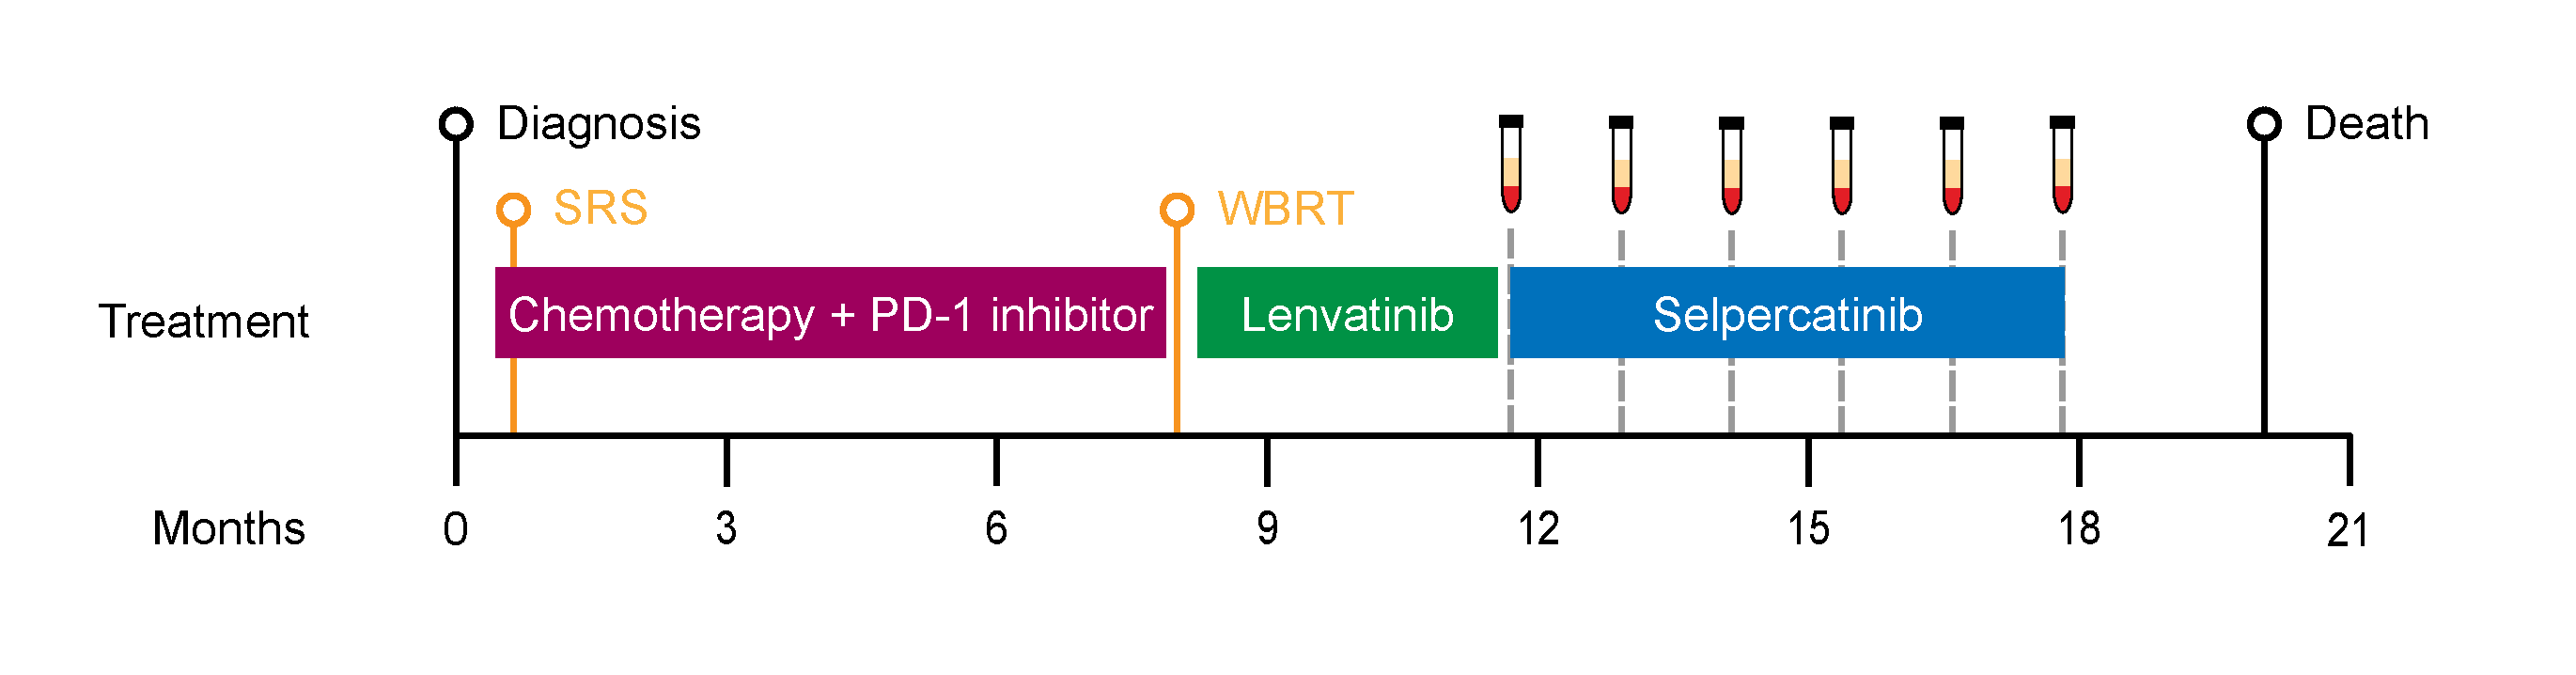
\includegraphics[width=.99\linewidth]{Figures/CASCADE/CA99/CA-A_timeline}
\caption[Timeline of patient CA-A from diagnosis until death]{Timeline of patient CA-A from diagnosis until death: Diagnostic biopsy detected \textit{KIF5B-RET} positive lung adenocarcinoma; SRS: stereotactic radiosurgery; WRBT: whole brain radiation therapy; a total of six blood samples were taken just before and during the selpercatinib treatment.} \label{fig:ca99timeline}
\end{figure}


Serial sampling of the plasma of the patient and analysis with the commercial Guardant360 assay \cite{Talasaz2014} revealed a previously undetected RET~G810S resistance mutation after three months of treatment . While at this point the driver mutation allele frequency was still dropping in the plasma, by month four the abundance of RET~G810S had increased and was accompanied by additional mutations in the same site (RET~G810R, C, and V). In addition there was an increase of fusion positive ctDNA this suggesting the development of acquired resistance to Selpercatinib. While the patient initially was responsive to the treatment, repeat PET scans showed progressive disease after six months, which ultimately led to the death of the patient (\autoref{fig:ca99pet}).

\begin{figure}[htp]
\centering
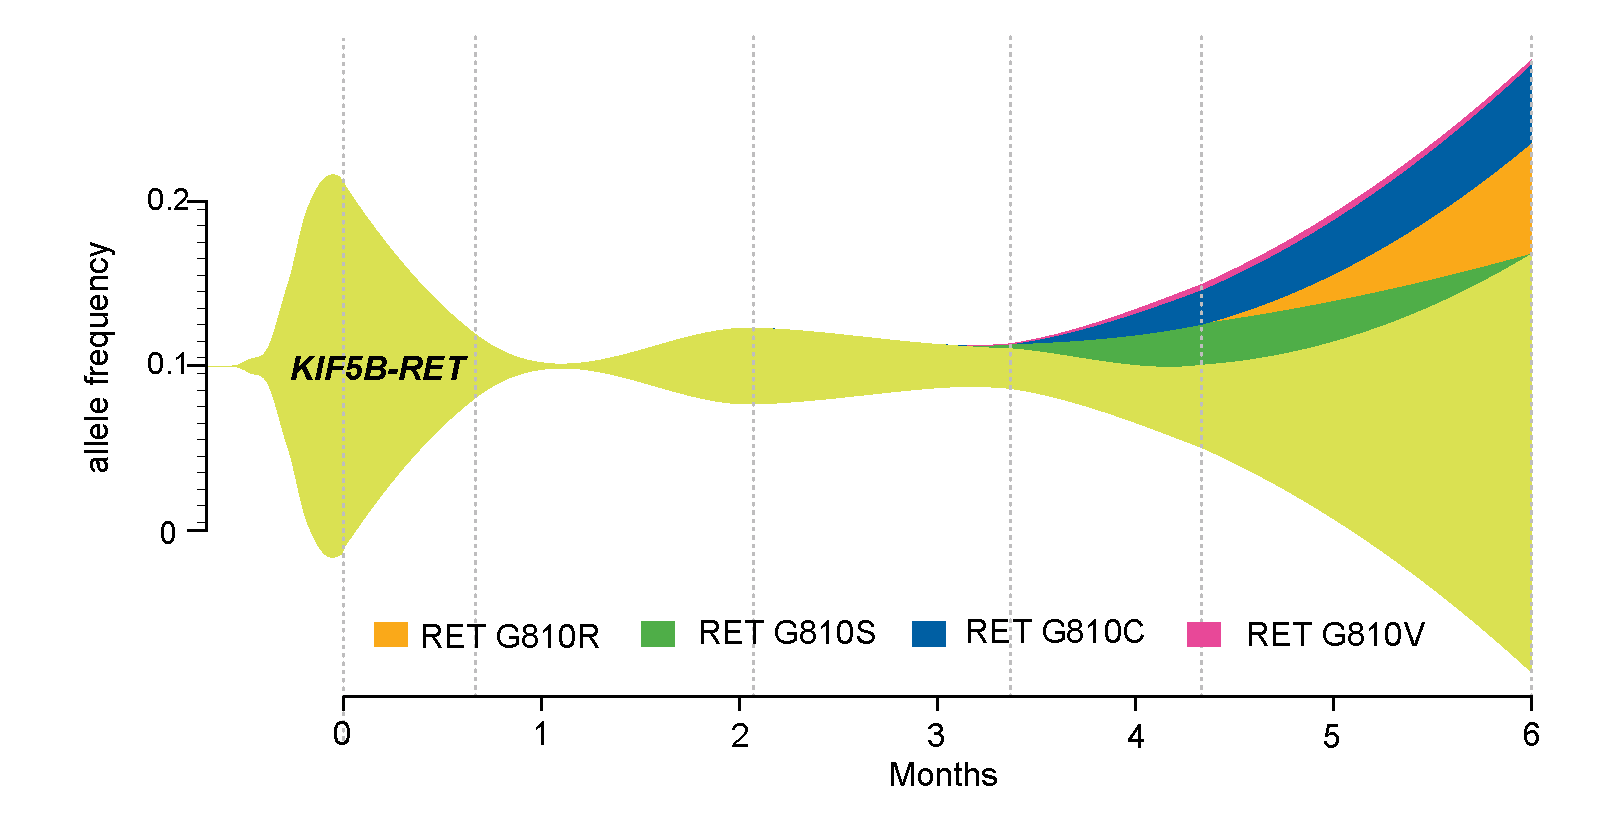
\includegraphics[width=.99\linewidth]{Figures/CASCADE/CA99/CA-A_ctDNAstream}
\caption[Allelic frequencies of driver and emerging resistance mutations]{Allelic frequencies of driver and emerging resistance mutations during Selpercatinib treatment (11 months after diagnosis); \textit{KIF5B-RET} fusion is the initiating driver with RET~G810R/S/C/V the emerging resistance SNPs} \label{fig:ca99ctDNA}
\end{figure}


\begin{figure}[hbp]
\centering
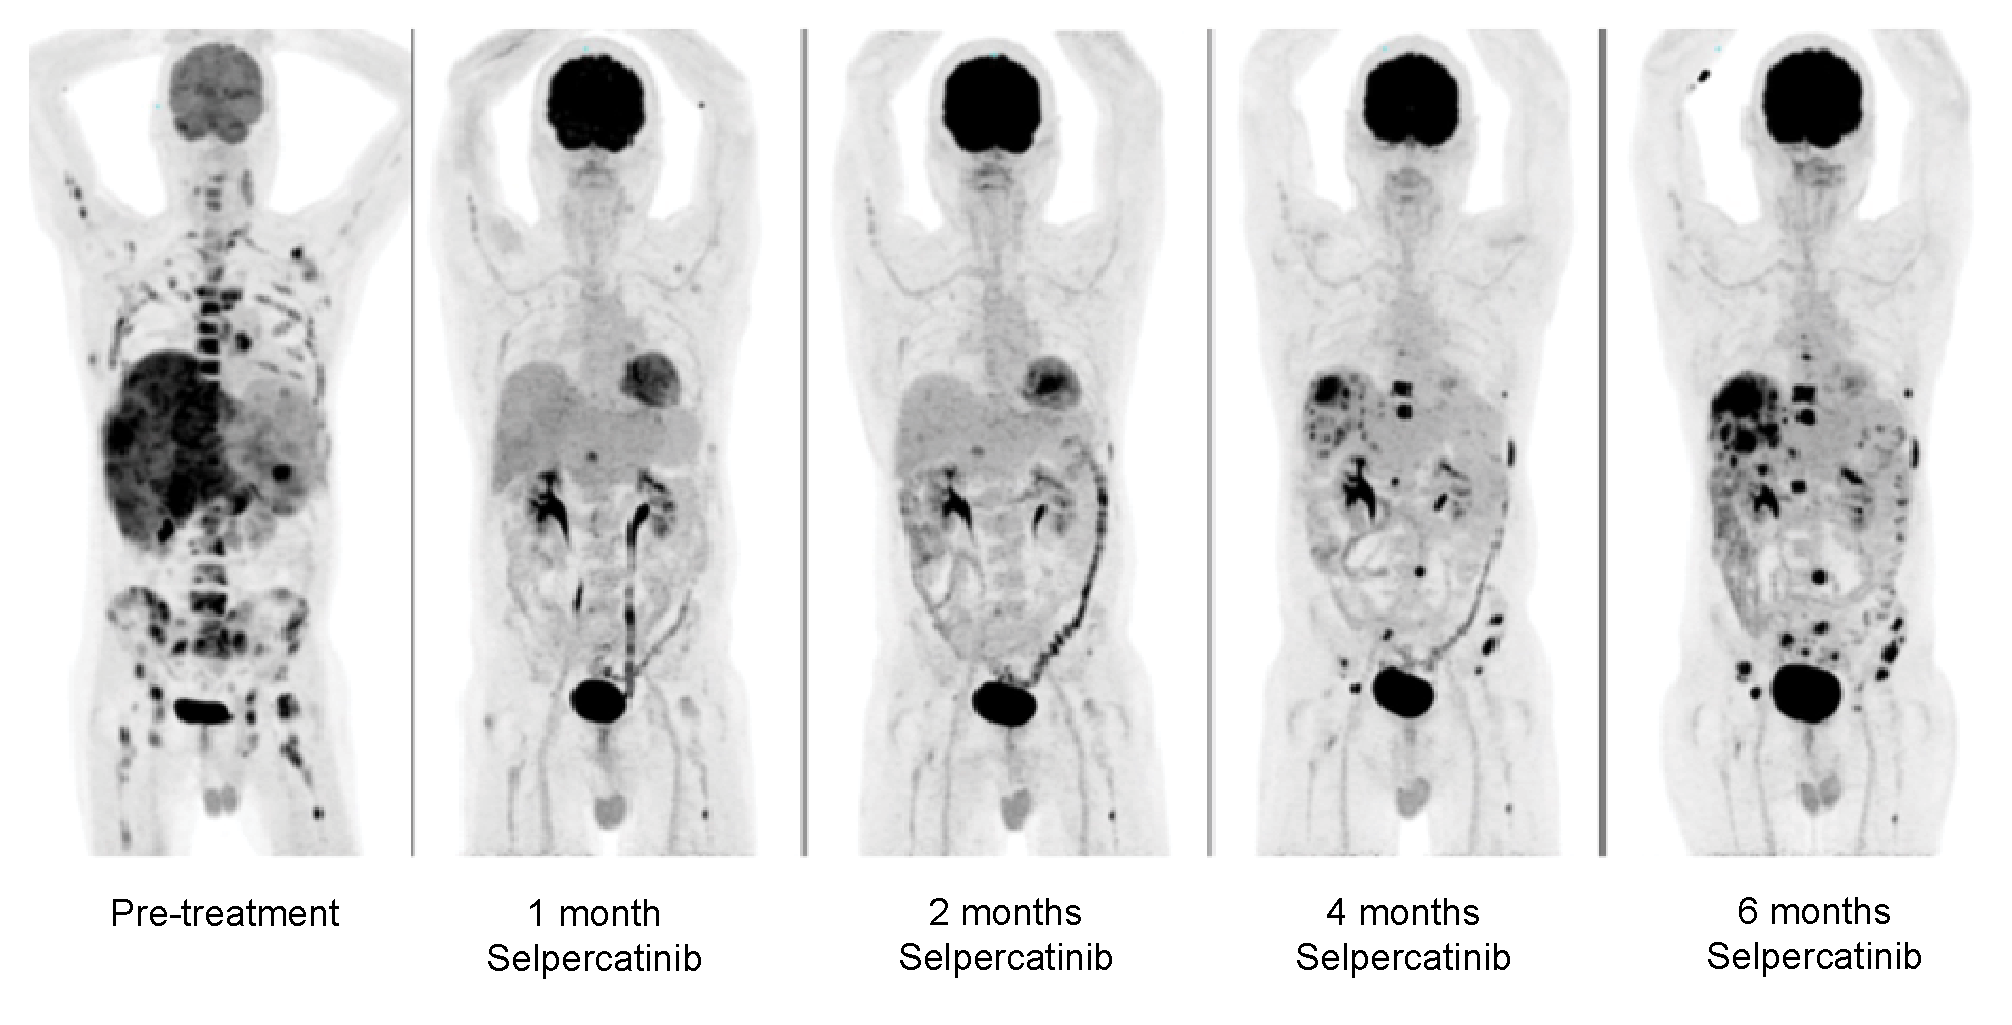
\includegraphics[width=.99\linewidth]{Figures/CASCADE/CA99/CA-A_PETscans}
\caption[PET scans of patient CA-A before and during Selpercatinib treatment]{PET scans of patient CA-A before and during Selpercatinib treatment} \label{fig:ca99pet}
\end{figure}


\begin{figure}[htp]
\centering
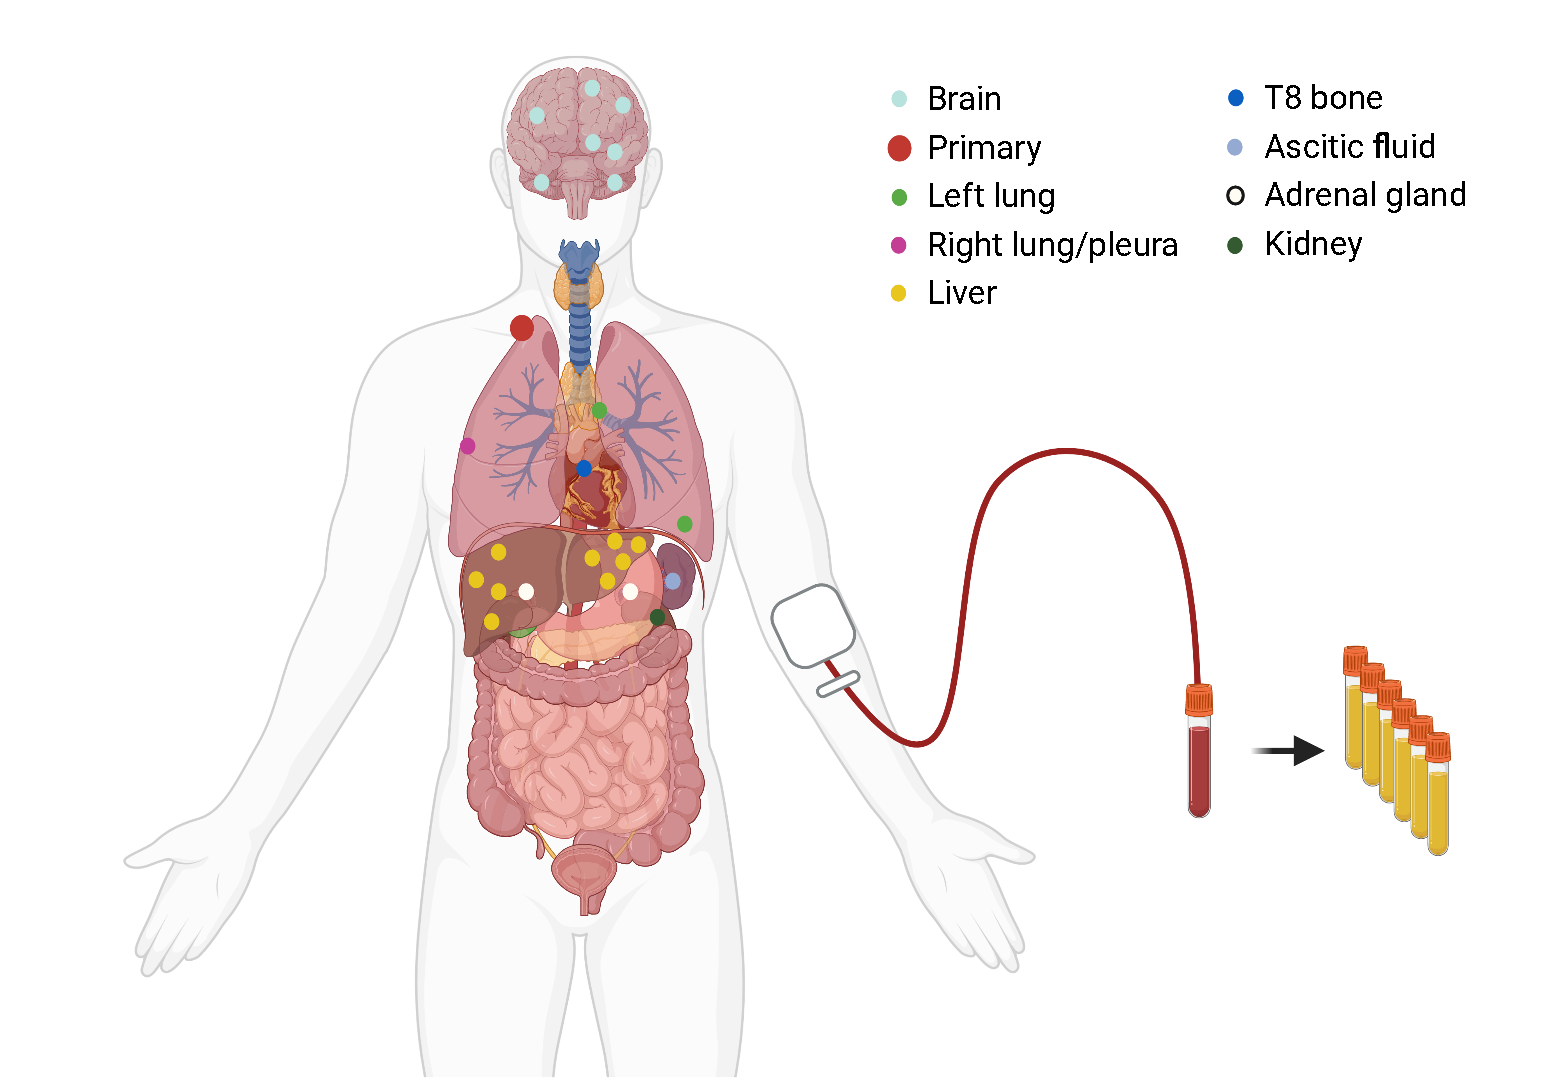
\includegraphics[width=.99\linewidth]{Figures/CASCADE/CA99/CA-A_schematic_CA99_organColours}
\caption[Schematic of tumour lesions in patient CA-A]{Schematic of tumour lesions in patient CA-A: Primary diagnostic sample shown in red; All 24 autopsy samples were coloured by organ they were collected from: Brain (7), left lung (2), right lung (1), liver (9), T8 bone (1), ascitic fluid (1), adrenal gland (2), kidney (1); Additionally to the post mortem blood sample, six serial blood samples were taken (\protect\autoref{fig:ca99timeline})} \label{fig:ca99schematic}
\end{figure}


At autopsy, 24 tumour tissue biopsies and a post mortem blood sample were collected and eight of them were selected for WGS at 130x coverage (\autoref{fig:ca99schematic}, \autoref{tab:ca99wgsSamples}) and analysed with the standard workflow (\autoref{cascade-sec:workflow}).

\begin{table}[ht]
\caption[Autopsy samples sequenced for patient CA-A]{Autopsy samples sequenced for patient CA-A: Sample number is the internal sample collection during CASCADE autopsy, the organ of the sample, the fraction of tumour cells from H\& E stain and the pathology of the tumour sample.}\label{tab:ca99wgsSamples}
\centering
\rowcolors{2}{gray!15}{white}
\begin{tabular}{|c|c|c|c|c|}
\toprule
\hline
 \rowcolor{gray!50}
\textbf{Sample number} & \textbf{Organ} & \textbf{H\&E} & \textbf{Type}\\
\hline
 11 & right occipital lobe & 0.7 &  \cellcolor{white}\\
 26 & right liver lobe & 0.6 & \cellcolor{white} \\
 31 & left lower lung & 0.2 & \cellcolor{white} \\
 41 & left liver lobe & 0.2 & \cellcolor{white} \\
 47 & left liver lobe & 0.5 & \cellcolor{white} \\
 55 & left liver lobe & 0.4 & \cellcolor{white} \\
 57 & right liver lobe & 0.6 & \cellcolor{white} \\
 59 & right pleura & 0.7 & \cellcolor{white}\multirow{-8}{*}{lung adenocarcinoma} \\
 \hline
\bottomrule
\end{tabular}
\end{table} 

Somatic variant calling revealed substantial spatial heterogeneity, where both the occipital lobe and the right pleura sample only contained RET~G810S, the right liver lobe harboured predominantly RET~G810R with either G810S and G810C as minor clones and lastly, the left liver samples showed almost an even mix between G810C and G810S clones but no G810R presence. The emergence of these mutations in multiple different sites at different allele frequencies, especially in already established sites in the liver, suggests that these mutations are the result of parallel evolution under positive selection through therapy, rather than seeding from one resistant clone.
Apart from the mutations changing RET~G810 no other variants affecting \textit{RET} or any other lung cancer genes were found in multiple samples. The occipital lobe sample also contained a BRCA1~V939A  mutation and one left liver sample (47) showed a synonymous KIT~S967\%3D mutation. Additionally, no other variant found in non cancer related genes allowed the same explanation of resistance (\autoref{fig:ca99heatmap}).

Phylogeny based on the short variants showed a clear clustering of the right (26 and 57) and left liver samples (41, 47, and 55) with the ocipital lobe (11) and pleural sample (59) sharing the most mutations as a hint towards the longest evolutionary trajectory and final progression. There was also a bifurcating line separating several progression (11, 41,47,55; top right) and stable disease sites. The much lower and higher number of both samples 31 and 41 may have been contributed to by the low tumour purity of those samples (\Autoref{tab:ca99wgsSamples,tab:ca99cnv}, \autoref{fig:ca99phylo}).

\begin{figure}[htp]
	\centering
	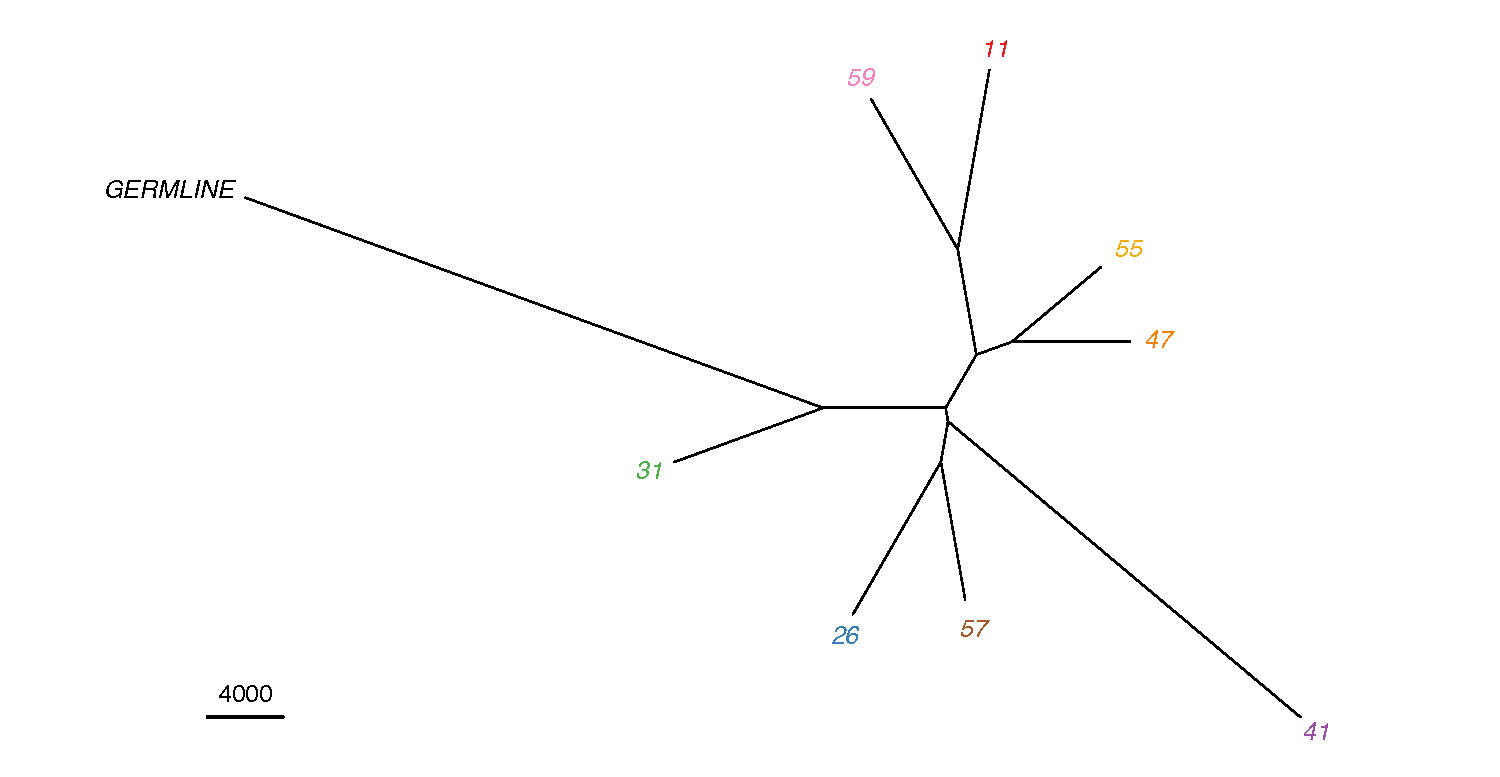
\includegraphics[width=.99\linewidth]{Figures/CASCADE/CA99/CA99phylo.pdf}
	\caption[Phylogeny of autopsy samples from patient CA-A]{Phylogeny of autopsy samples from patient CA-A; reconstructed with all somatic SNVs and InDels. Ruler symbolises 4000 variants difference} \label{fig:ca99phylo}
\end{figure}

\begin{figure}[htp]
\centering
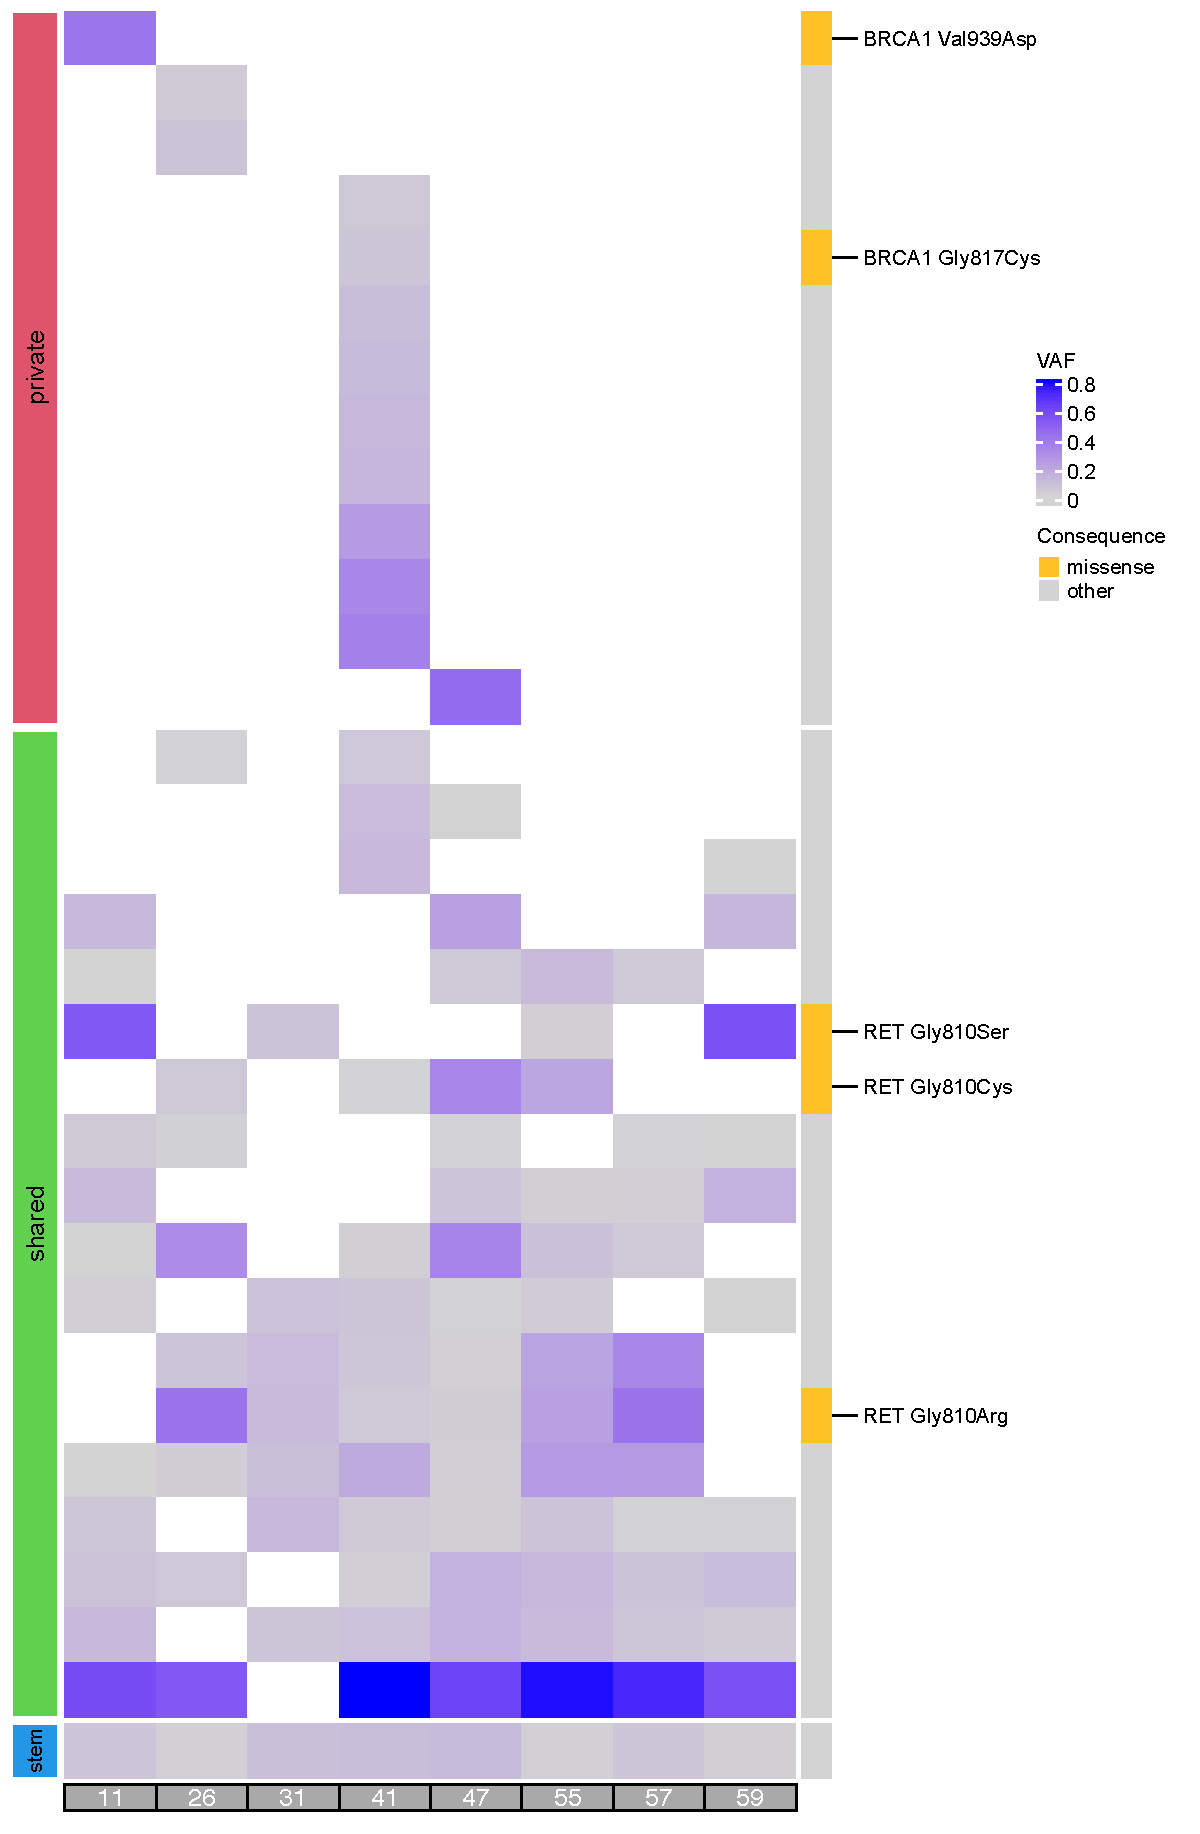
\includegraphics[width=.99\linewidth]{Figures/CASCADE/CA99/CA99varHeatmap.pdf}
\caption[Heatmap of driver gene variants in patient CA-A]{Heatmap of driver gene variants in patient CA-A: Protein altering mutations are highlighted with their HGVSp notation; non protein altering mutations are grouped as ``other``.} \label{fig:ca99heatmap}
\end{figure}



The structural variant calling with GRIDSS2 showed consistent presence of the \textit{KIF5B-RET} fusion at high allele frequency (min: 0.27 max: 0.535), consistent with a cancer cell fraction of 1 when correcting for local copy number changes  (min: 2 max: 3; \autoref{fig:ca99.11circos}), in all but sample 31, which might have been due to the low purity of the sample (\autoref{tab:ca99wgsSamples}). While there was a high number of structural variants present in each sample, consistent with the genomic instability commonly seen in late stages of cancer \cite{Gerstung2020} almost of these rearrangements were sub-clonal and therefore not the main cause of resistance or cancer initiation and rather the result of progressive tumour evolution. To allow a more focused look at structural events and their effect, we restricted the visualisation to events with an allele frequency of 0.2 or higher (\Autoref{fig:ca99.11circos,fig:ca99.11circosnoAF}).

While this change also has a minute effect on the PURPLE copy number calls, which are informed by structural variants, these structural variants will also be sub-clonal and therefore removal will result in a cleaner clonal copy number profile.


\begin{figure}[htp]
\centering
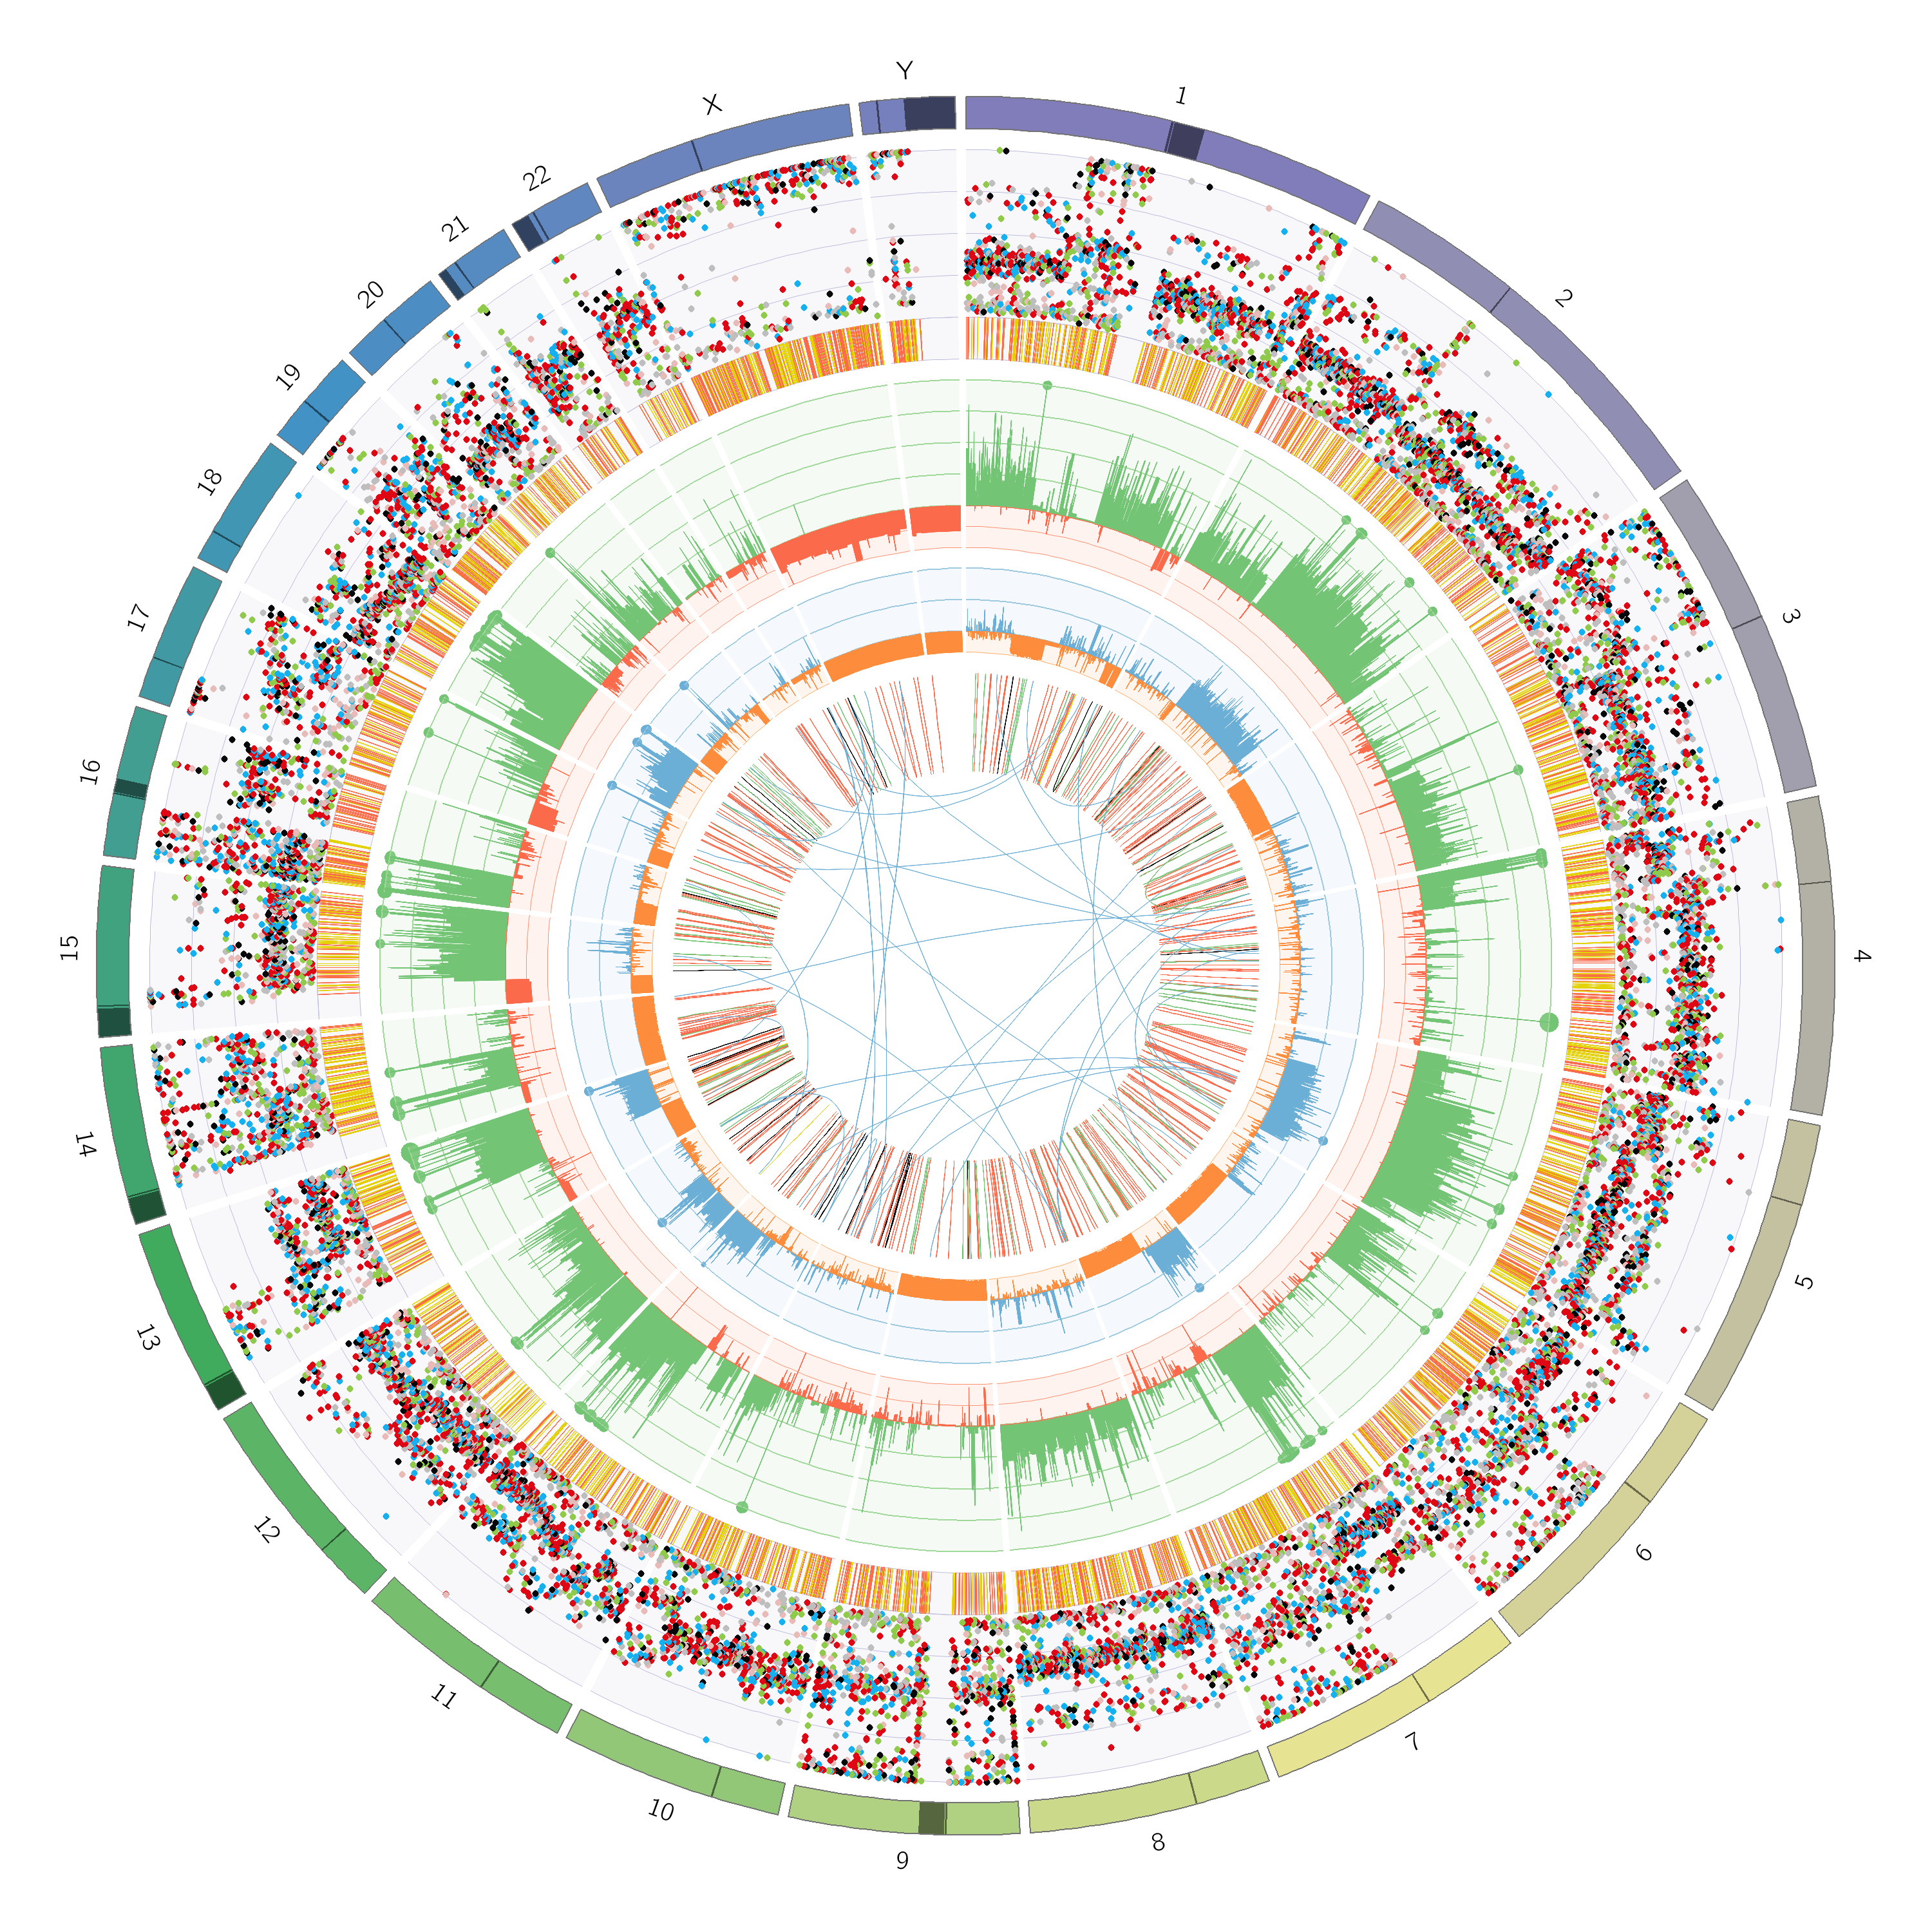
\includegraphics[width=.99\linewidth]{Figures/CASCADE/CA99/CA99-11.circos.png}
\caption[Circos plot of patient CA-A sample 11]{Circos plot of patient CA-A with somatic structural variants with allele frequency $> 0.2$: outer first ring shows the canonical chromosomes with gaps (centromere, heterochromatin,...) highlighted as darker areas; second ring visualises all somatic SNVs corrected for tumour purity and scaled from 0 to 1, the colour representing the base change of SNV like in \protect\textcite{Alexandrov2013}; vertical lines directly under the SNVs symbolise InDels, with yellow for insertions and red for deletions; the third ring shows the total copy number alterations, with green showing a copy number gain and red a loss, dots at the outer border show a copy number greater than four; the last ring shows the minor copy number, with blue depicting a gain and orange a loss, this ring allows the detection of copy number neutral changes, like loss of heterozygosity; the center shows all structural variants: translocations in blue, deletions in red, insertions in yellow, tandem duplications in green and inversions in black.} \label{fig:ca99.11circos}
\end{figure}


\begin{figure}[htp]
\centering
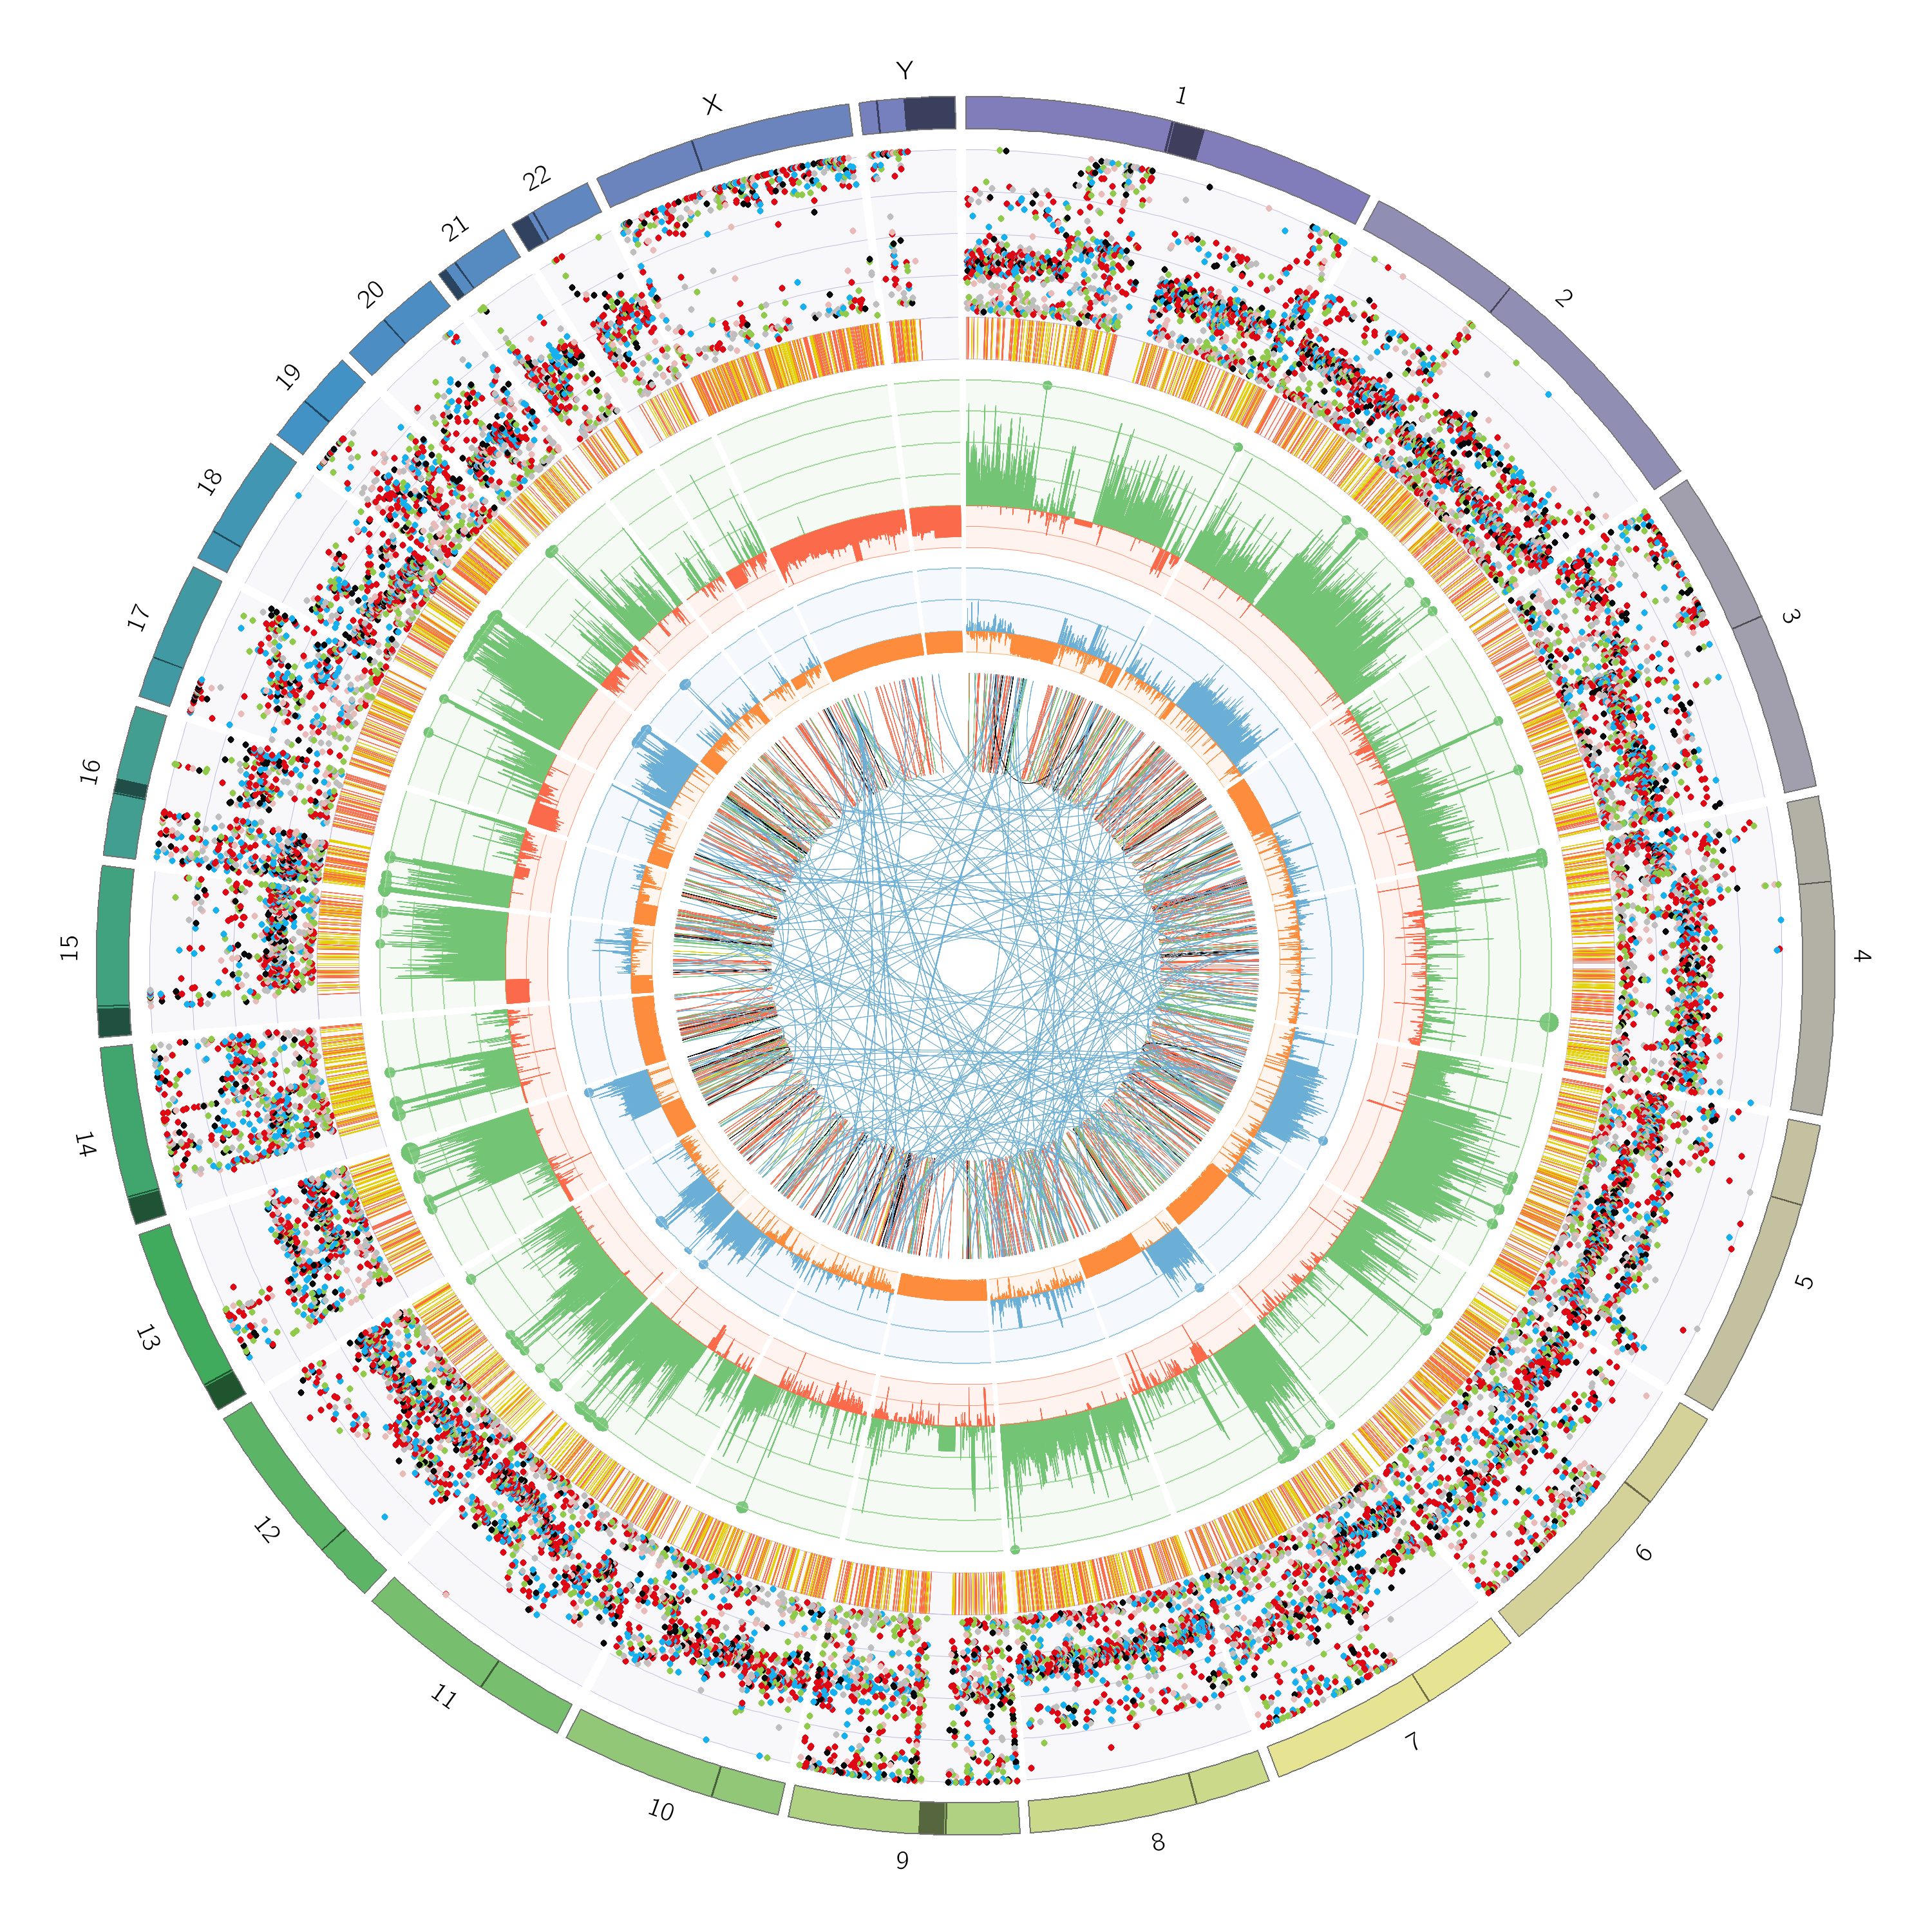
\includegraphics[width=.99\linewidth]{Figures/CASCADE/CA99/CA99-11.circos_0.05AF.png}
\caption[Circos plot of patient CA-A sample 11 without allele frequency filter]{Circos plot of patient CA-A with all somatic structural variants: outer first ring shows the canonical chromosomes with gaps (centromere, heterochromatin,...) highlighted as darker areas; second ring visualises all somatic SNVs corrected for tumour purity and scaled from 0 to 1, the colour representing the base change of SNV like in \protect\textcite{Alexandrov2013}; vertical lines directly under the SNVs symbolise InDels, with yellow for insertions and red for deletions; the third ring shows the total copy number alterations, with green showing a copy number gain and red a loss, dots at the outer border show a copy number greater than four; the last ring shows the minor copy number, with blue depicting a gain and orange a loss, this ring allows the detection of copy number neutral changes, like loss of heterozygosity; the center shows all structural variants: translocations in blue, deletions in red, insertions in yellow, tandem duplications in green and inversions in black.} \label{fig:ca99.11circosnoAF}
\end{figure}

%think about putting the circos plot on one page, height=.4\textheight, keepaspectratio

\Autoref{fig:ca99.11circos,fig:ca99.26circos,fig:ca99.41circos,fig:ca99.47circos,fig:ca99.55circos,fig:ca99.57circos,fig:ca99.59circos} show very similar copy number profiles of all tumour samples of patient CA-A, with loss of heterozygosity on almost all chromosomes apart from chromosome 5 and 9. Only \autoref{fig:ca99.26circos} showed a less granular mix of gain and loss of the minor allele, which was most likely due to the lower tumour purity of the sample. However, all samples exhibited high copy number gain levels consistent with whole genome duplication (\Autoref{tab:ca99wgsSamples,tab:ca99cnv}). All samples showed a copy number gain in chromosome 7 at the \textit{EGFR} locus leading to \textit{EGFR} amplification (min: 3.9 max: 9.9), which is a known resistance mechanism to Levantinib \cite{Jin2021} and was therefore most likely a result of previous treatment (\autoref{fig:ca99timeline}). Just as expected from the results of the Guardant360 ctDNA results leading up to the death of the patient, there was no \textit{MET} amplification present in the patient at any site.

With the absence of any other plausible mechanism, of SNV, SV or CNV nature, the only possible explanation of resistance to Selpercatinib in the patient was the solvent front mutations RET~G810C, G810R, G810S, and G810V as described in \textcite{Solomon2020}. However, the autopsy revealed substantial spatial heterogeneity of the emerged resistance mechanisms within the patient which was previously unappreciated.

\begin{table}[ht]
\caption[Copy number analysis results for patient CA-A]{Copy number analysis results for patient CA-A: results are taken from the best fit result of PURPLE; WG: whole genome}\label{tab:ca99cnv}
\centering
\rowcolors{2}{gray!15}{white}
\begin{tabular}{|c|c|c|c|c|}
\toprule
\hline
 \rowcolor{gray!50}
\textbf{Sample number} & \textbf{purity} & \textbf{ploidy} & \textbf{polyclonal \%} & \textbf{WG duplication}\\
\hline
 11 & \num{0.73} &	 \num{2.86} &	\num{29.75} & \cellcolor{white}	\\
 26 & \num{0.61} & \num{3.00} & \num{26.57} & \cellcolor{white} \\
 31 & \num{0.21} & \num{5.40} & \num{49.86} & \cellcolor{white} \\
 41 & \num{0.28} & \num{4.30} & \num{42.43} & \cellcolor{white} \\
 47 & \num{0.46} & \num{2.86} & \num{29.72} & \cellcolor{white} \\
 55 & \num{0.38} & \num{2.86} & \num{38.41} & \cellcolor{white} \\
 57 & \num{0.61} & \num{3.00} & \num{28.55} & \cellcolor{white} \\
 59 & \num{0.69} & \num{2.60} & \num{37.11} & \cellcolor{white}\multirow{-8}{*}{True} \\
 \hline
\bottomrule
\end{tabular}
\end{table} 



With the high percentage of likely sub-clonality of samples (\Autoref{tab:ca99cnv}) we used PhylogicNDT to infer clonal hierarchy and complexity. Initial analysis confirmed 141 clone like clusters, which far exceeded the maximum amount PhylogicNDT was able to visualise. In \autoref{fig:ca99.ccfCluster} the clonal abundance per sample for the three clones 64, 70 and 139 was shown, which corresponded to RET~G810C, RET~G810R, and RET~G810S respectively, exactly as seen in the longitudinal data (\autoref{fig:ca99ctDNA}). The clonal abundance in each sample was highly variable and followed an exclusion pattern, where if one resistant clone was present another was not. Only sample 31 and 55 showed signs of mixed populations. We attributed these patterns to parallel evolution due to selection pressure of the drug on already established lesions rather than metastatic seeding.

\begin{figure}[htp]
\centering
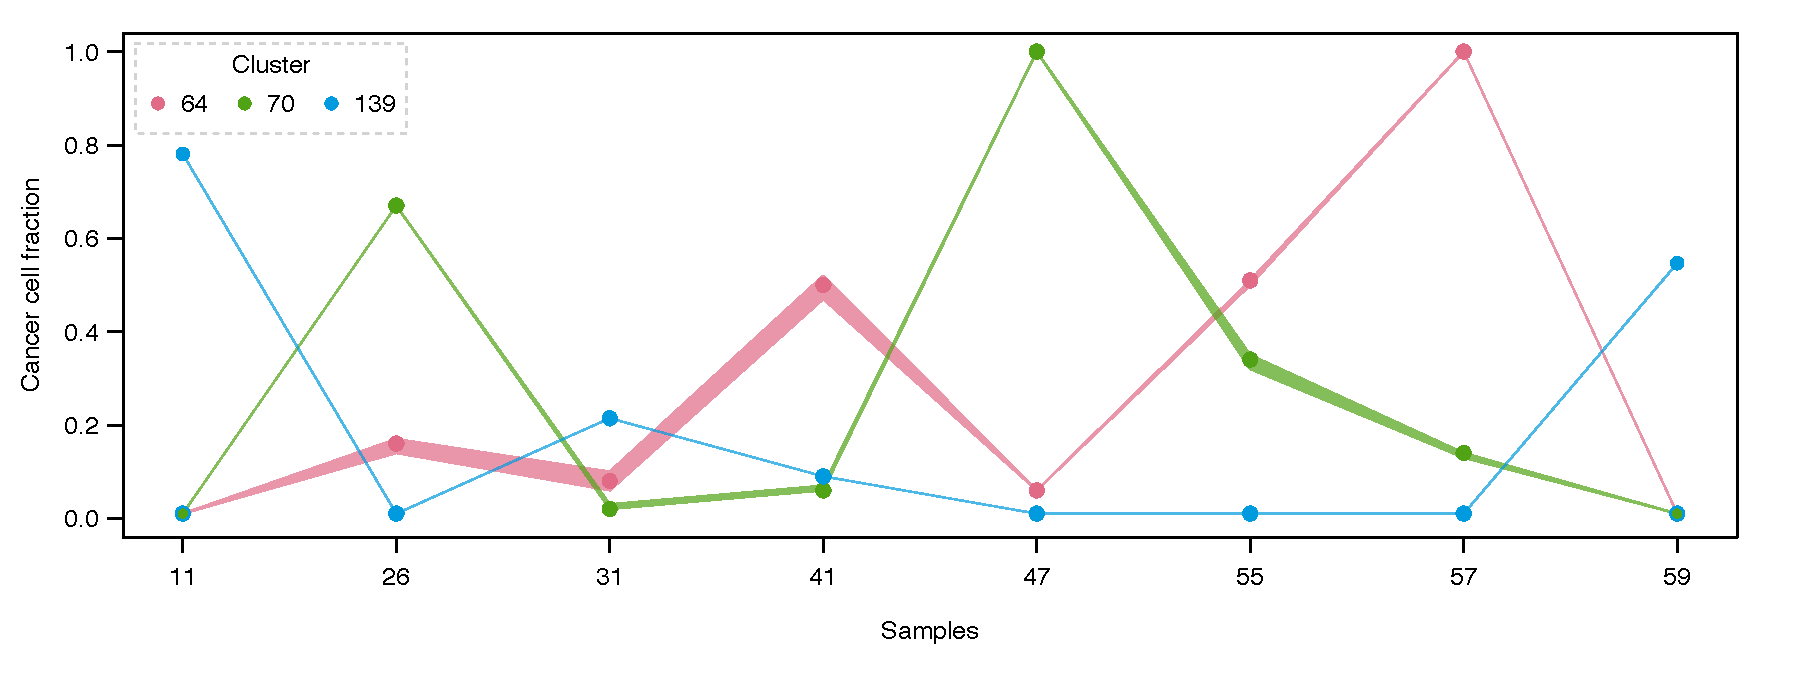
\includegraphics[width=.99\linewidth]{Figures/CASCADE/CA99/CA99.ccf_cluster.pdf}
\caption[Cancer cell fraction of mutation clusters of clonal tree for patient CA-A]{Cancer cell fraction of mutation clusters for patient CA-A; transparent polygons show the 95\% confidence intervals. Clusters were generated with PhylogicNDT} \label{fig:ca99.ccfCluster}
\end{figure}

We attempted to build a clonal tree from the clustered mutations with PhylogicNDT with the restricted clusters using \autoref{eq:clusterRestriction}, however no output was generated after 480 CPU hours. In contrast all other patients required less than 100 CPU hours. We assumed the high subclonality of the data made it impossible to converge to a solution. This again highlights the necessity of computational methods to close the gap between current algorithms and the available datasets.



%we clear all floats before we go to the next patient
\cleardoublepage


%%%%%%%%%%%%%%%%%%%%%%%%%%%%%%%%%%%%%%%%%%%%%%%%%%%%%%%%%%%%%%%%%%%%%%%%%%%%%%%%%%%%%%%
%                               Patient CA51                                          %
%%%%%%%%%%%%%%%%%%%%%%%%%%%%%%%%%%%%%%%%%%%%%%%%%%%%%%%%%%%%%%%%%%%%%%%%%%%%%%%%%%%%%%%


\subsection{Patient CA-I}
\label{cascade-sec:CA51}

This 56 year old female never smoker presented with an \textit{EGFR} exon 19 deletion positive NSCLC in stage IV with metastatic involvement. After an initial good response to Gefitinib treatment, the patient showed progressive nodal disease and was treated with Carboplatin/Gemcitabine chemotherapy with mixed response. After the change to the tyrosine kinase inhibitor Afatinib small intra-cranial metastases were detected and biopsy of a parasternal mass revealed small cell transformation in addition to the EGFR~T790M resistance mutation. Subsequent treatment changes to Carboplatin/Etoposide as well as CAV (cyclophosphamide, doxorubicin, vincristine) and finally Nivolumab were not successful and the patient died 40 months after diagnosis (\autoref{fig:ca51timeline}).

\begin{figure}[ht]
	\centering
	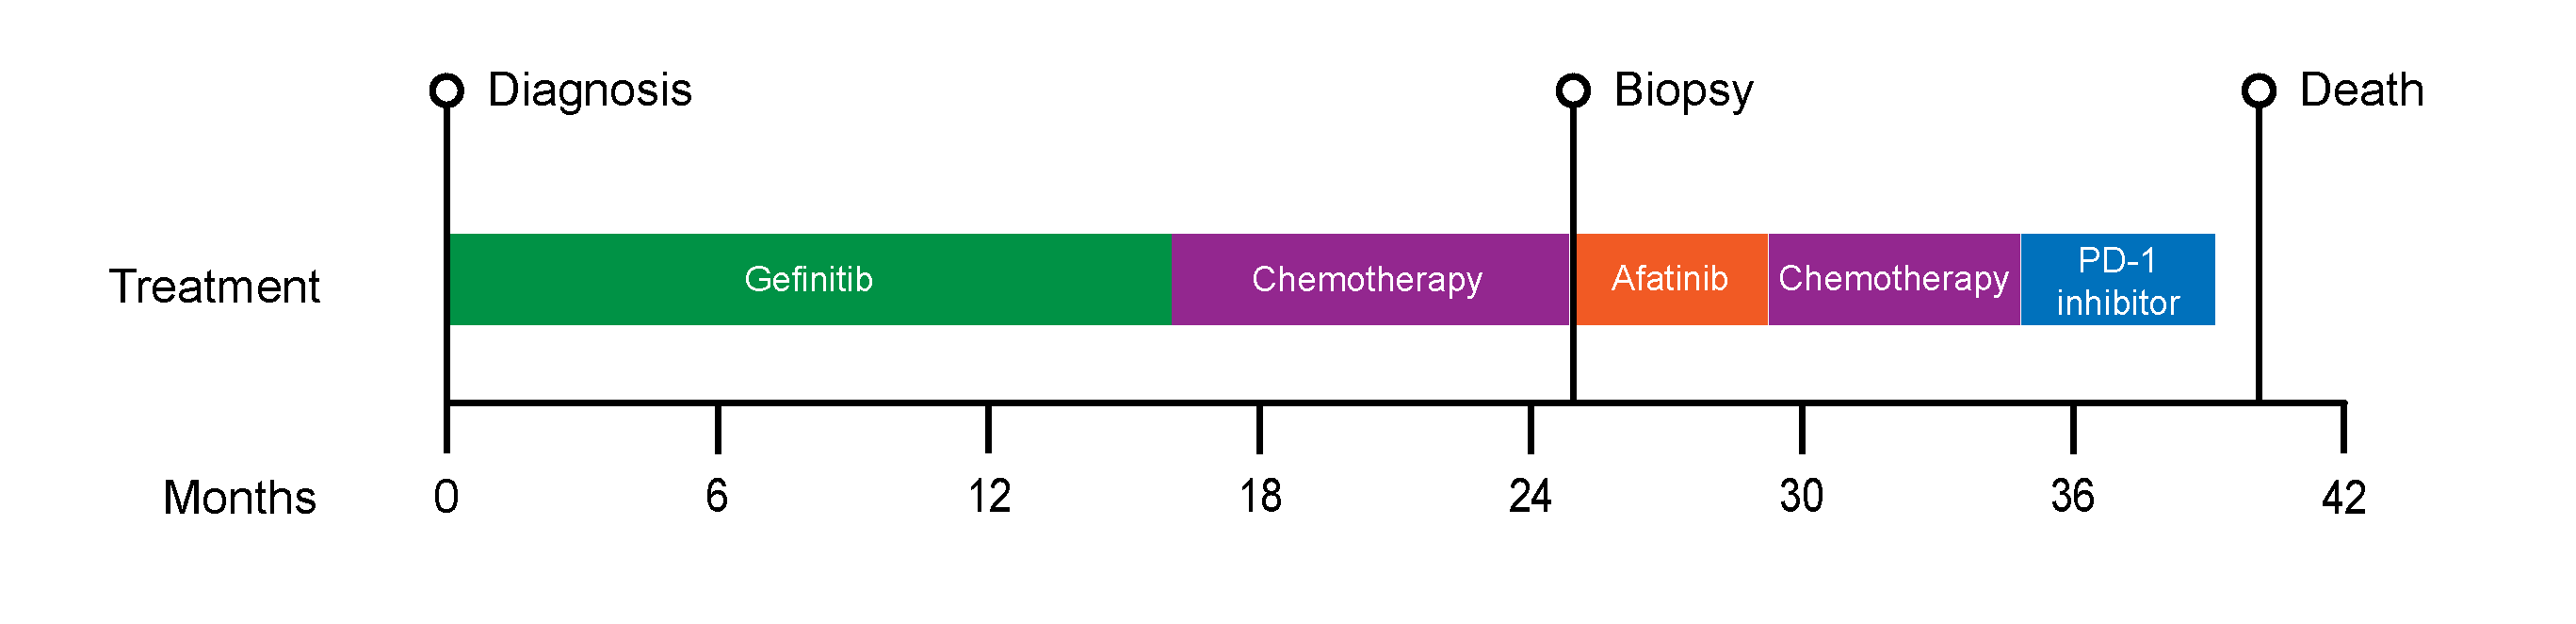
\includegraphics[width=.99\linewidth]{Figures/CASCADE/CA51/CA-I_timeline}
	\caption[Timeline of patient CA-I from diagnosis until death]{Timeline of patient CA-I from diagnosis until death: Diagnostic biopsy detected EGFR exon 19 deletion lung adenocarcinoma; Second biopsy after 24 months revealed additional EGFR~T790M mutation and small cell transformation} \label{fig:ca51timeline}
\end{figure}

At autopsy six lesions and one blood sample were collected and biobanked (\autoref{fig:ca51schematic}). After quality assessment by pathology with H\&E stain, all autopsy samples and the initial diagnostic biopsy were sequenced with WES (\autoref{tab:ca51wesSamples}) and analysed with the standard workflow (\autoref{cascade-sec:workflow}). The secondary small cell confirmation biopsy at 29 months did not contain enough tissue for sequencing.

\begin{figure}[htp]
	\centering
	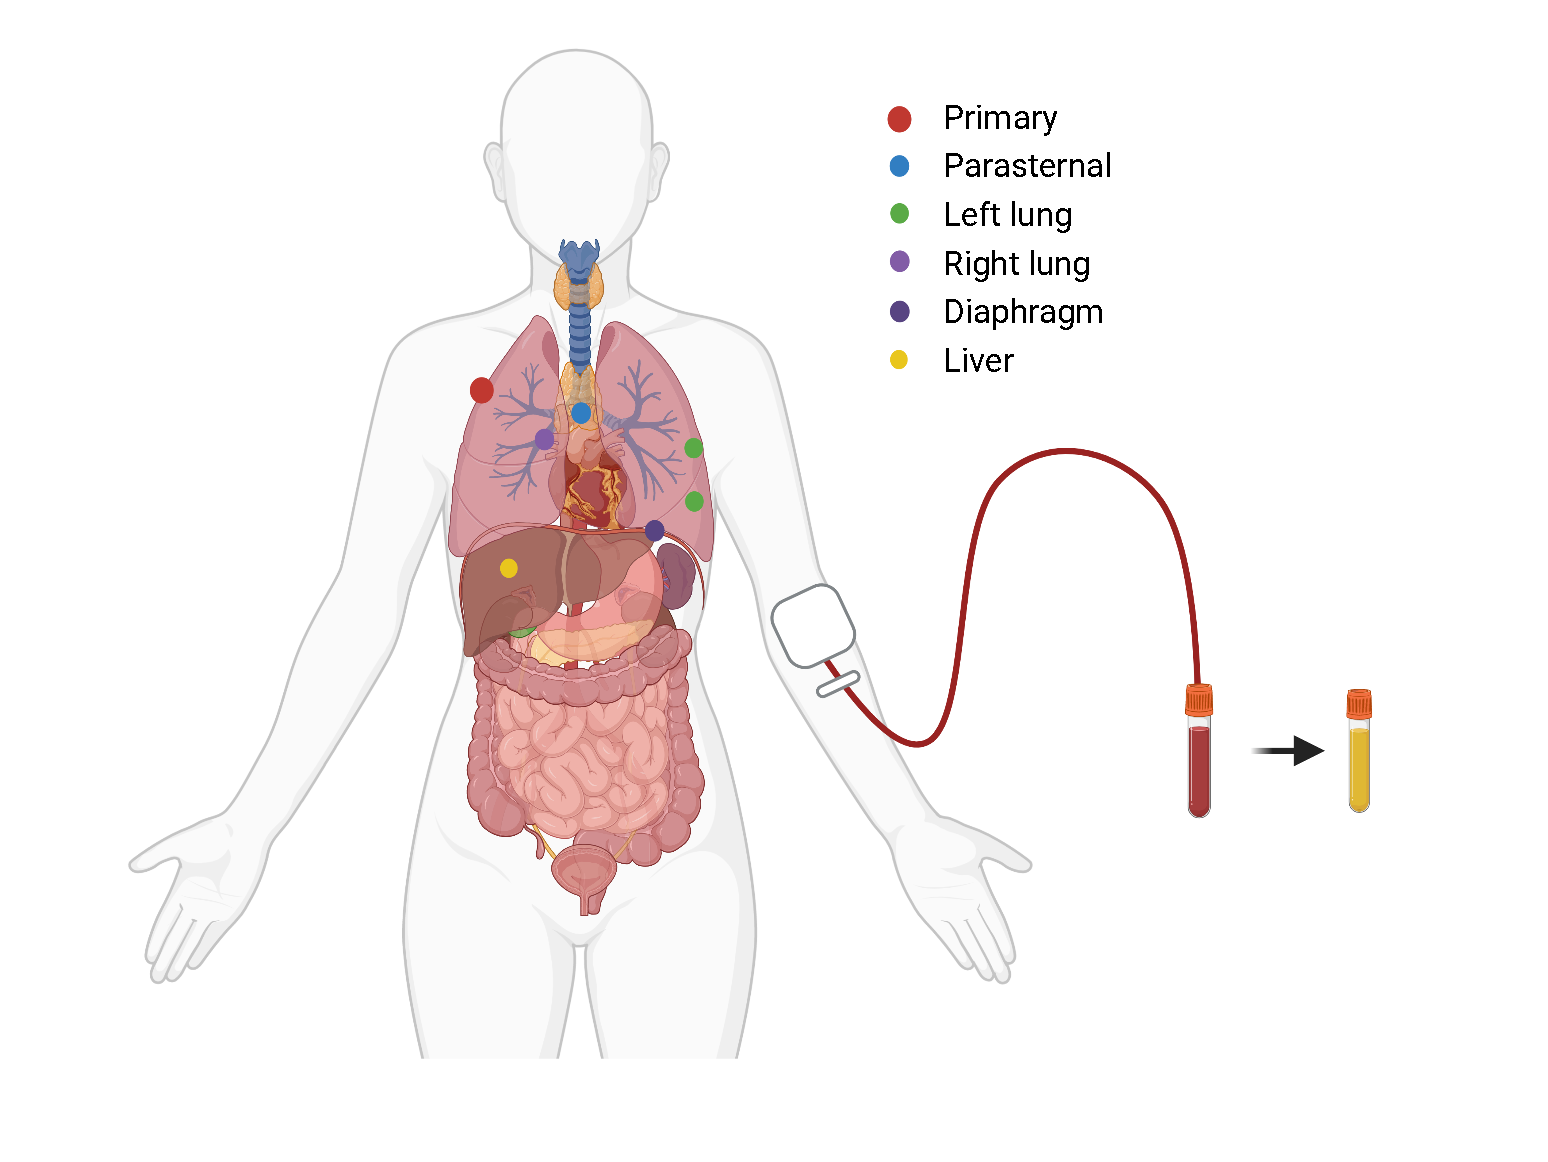
\includegraphics[width=.99\linewidth]{Figures/CASCADE/CA51/CA-I_schematic_CA51_organColours}
	\caption[Schematic of tumour lesions in patient CA-I]{Schematic of tumour lesions in patient CA-I: Primary diagnostic sample shown in red; All six autopsy samples were coloured by organ they were collected from: Parasternal (1), left lung (2), right lung (1), diaphragm (1), liver (1); Additionally a post mortem blood sample was taken} \label{fig:ca51schematic}
\end{figure}


\begin{table}[ht]
	\caption[Autopsy samples sequenced for patient CA-I]{Autopsy samples sequenced for patient CA-I: Sample number is the internal sample collection during CASCADE autopsy, the organ of the sample, the fraction of tumour cells from H\& E stain and the pathology of the tumour sample. Dx: diagnostic sample} \label{tab:ca51wesSamples}
	\centering
	\rowcolors{2}{gray!15}{white}
	\begin{tabular}{|c|c|c|c|c|}
	\toprule
	\hline
 	\rowcolor{gray!50}
\textbf{Sample number} & \textbf{Organ} & \textbf{H\&E} & \textbf{Type}\\
	\hline
 Dx & right VATS & - &  adenocarcinoma \\
 557 & parasternal mass & 0.9 & \cellcolor{gray!15} \\
 559 & left diaphragm & 0.9 & \cellcolor{gray!15} \\
 566 & right liver lobe & 0.6 & \cellcolor{gray!15} \\
 573 & right hilar lymph node & 0.9 & \cellcolor{gray!15} \\
 579 & left lung lobe & 0.8 & \cellcolor{gray!15} \\
 583 & left pleura & 0.9 & \cellcolor{gray!15}\multirow{-6}{*}{small cell} \\
 	\hline
	\bottomrule
	\end{tabular}
\end{table} 


Somatic variant calling showed very little genetic heterogeneity. The original \textit{EGFR} exon 19 deletion was present in all sequenced samples from the diagnostic sample to the 40 months later autopsy samples. No other protein altering somatic mutations were detected at a purity corrected allele frequency $\geq 0.33$. While the diagnostic sample presented with a TERT~H687Q mutation at 25\% VAF and sufficient local copy number amplification for 100\% cancer cell fraction, none of the autopsy samples showed any support for this variant. Generally, the number of somatic protein altering SNVs and InDels (min: 988 max: 1236 mean: 1090.5)  was very close to the average lung adenocarcinoma with an observed tumour mutational burden of 18.75 \cite{Alexandrov2013}. 
In contrast, the diagnostic sample showed a much higher number of mutations, which we attribute to the formalin-fixed paraffin-embedded (FFPE) preservation, which is known to cause DNA damage \cite{Do2015}. This DNA damage could have led to a higher rate of called somatic variants (\autoref{fig:ca51numVars}). In order to appreciate the relationship of the autopsy samples, we removed the diagnostic sample from the phylogenetic analysis. The full phylogeny can be seen in \autoref{fig:ca51phyloWithDx}. The phylogeny of SNVs and InDels shows no internal hierarchical structure, but rather shows that both the stem of tumour initiation and additional private mutations accumulated during the disease progression were approximately equal in number, with the stem being slightly longer. Only a very limited number of somatic variants were shared between cancer samples, which were not part of the initial stem (\autoref{fig:ca51phylo}). This was consistent with the clinical history, where there was never any clinical remission to treatment, but only mixed response in a subset of already established lesions.

\begin{figure}[htp]
	\centering
	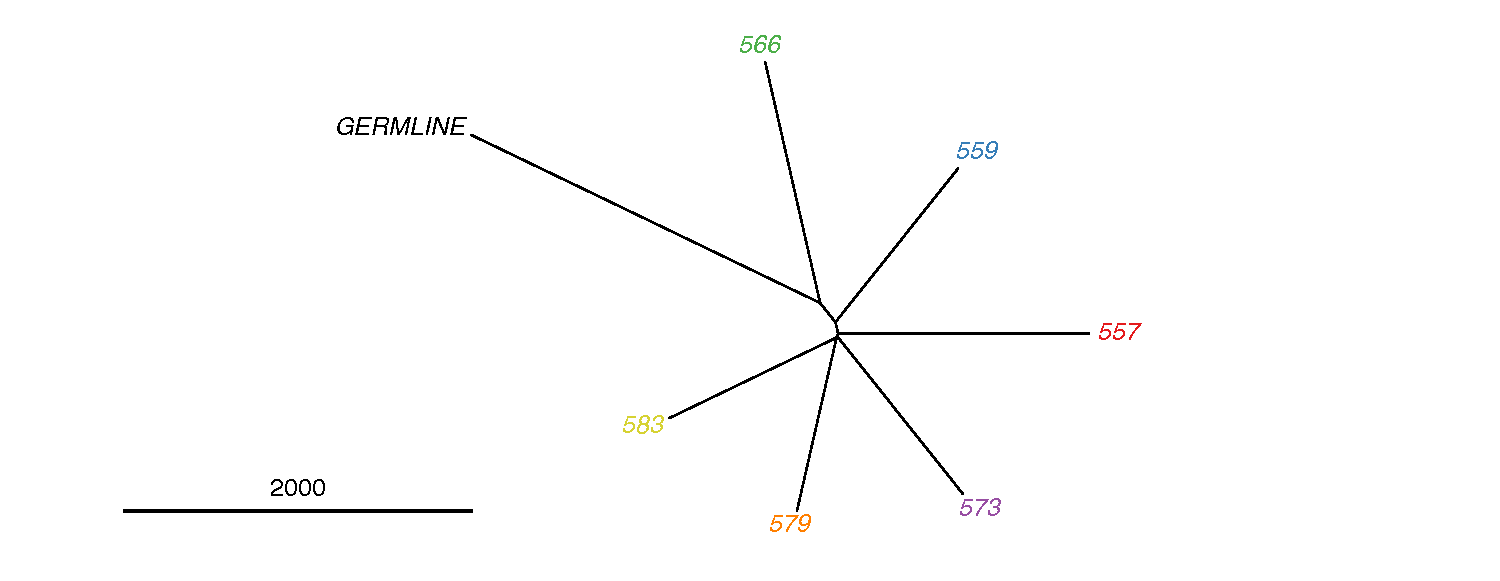
\includegraphics[width=.99\linewidth]{Figures/CASCADE/CA51/CA51phyloAutopsy.pdf}
	\caption[Phylogeny of autopsy samples from patient CA-I]{Phylogeny of autopsy samples from patient CA-I; reconstructed with all somatic SNVs and InDels. Ruler symbolises 2000 variants difference. The phylogeny with diagnostic sample can be found in \protect\autoref{fig:ca51phyloWithDx}} \label{fig:ca51phylo}
\end{figure}

In keeping with the small cell transformation, we could highlight an intronic \textit{TP53} mutations, which was present at almost 100\% VAF in all autopsy samples. However, the same variant was also found in the diagnostic sample, which was reportedly adenocarcinoma. The variant was therefore not sufficient to drive the transformation, but could have been a predisposition for the patient (\autoref{fig:ca51heatmap}).


\begin{figure}[htp]
\centering
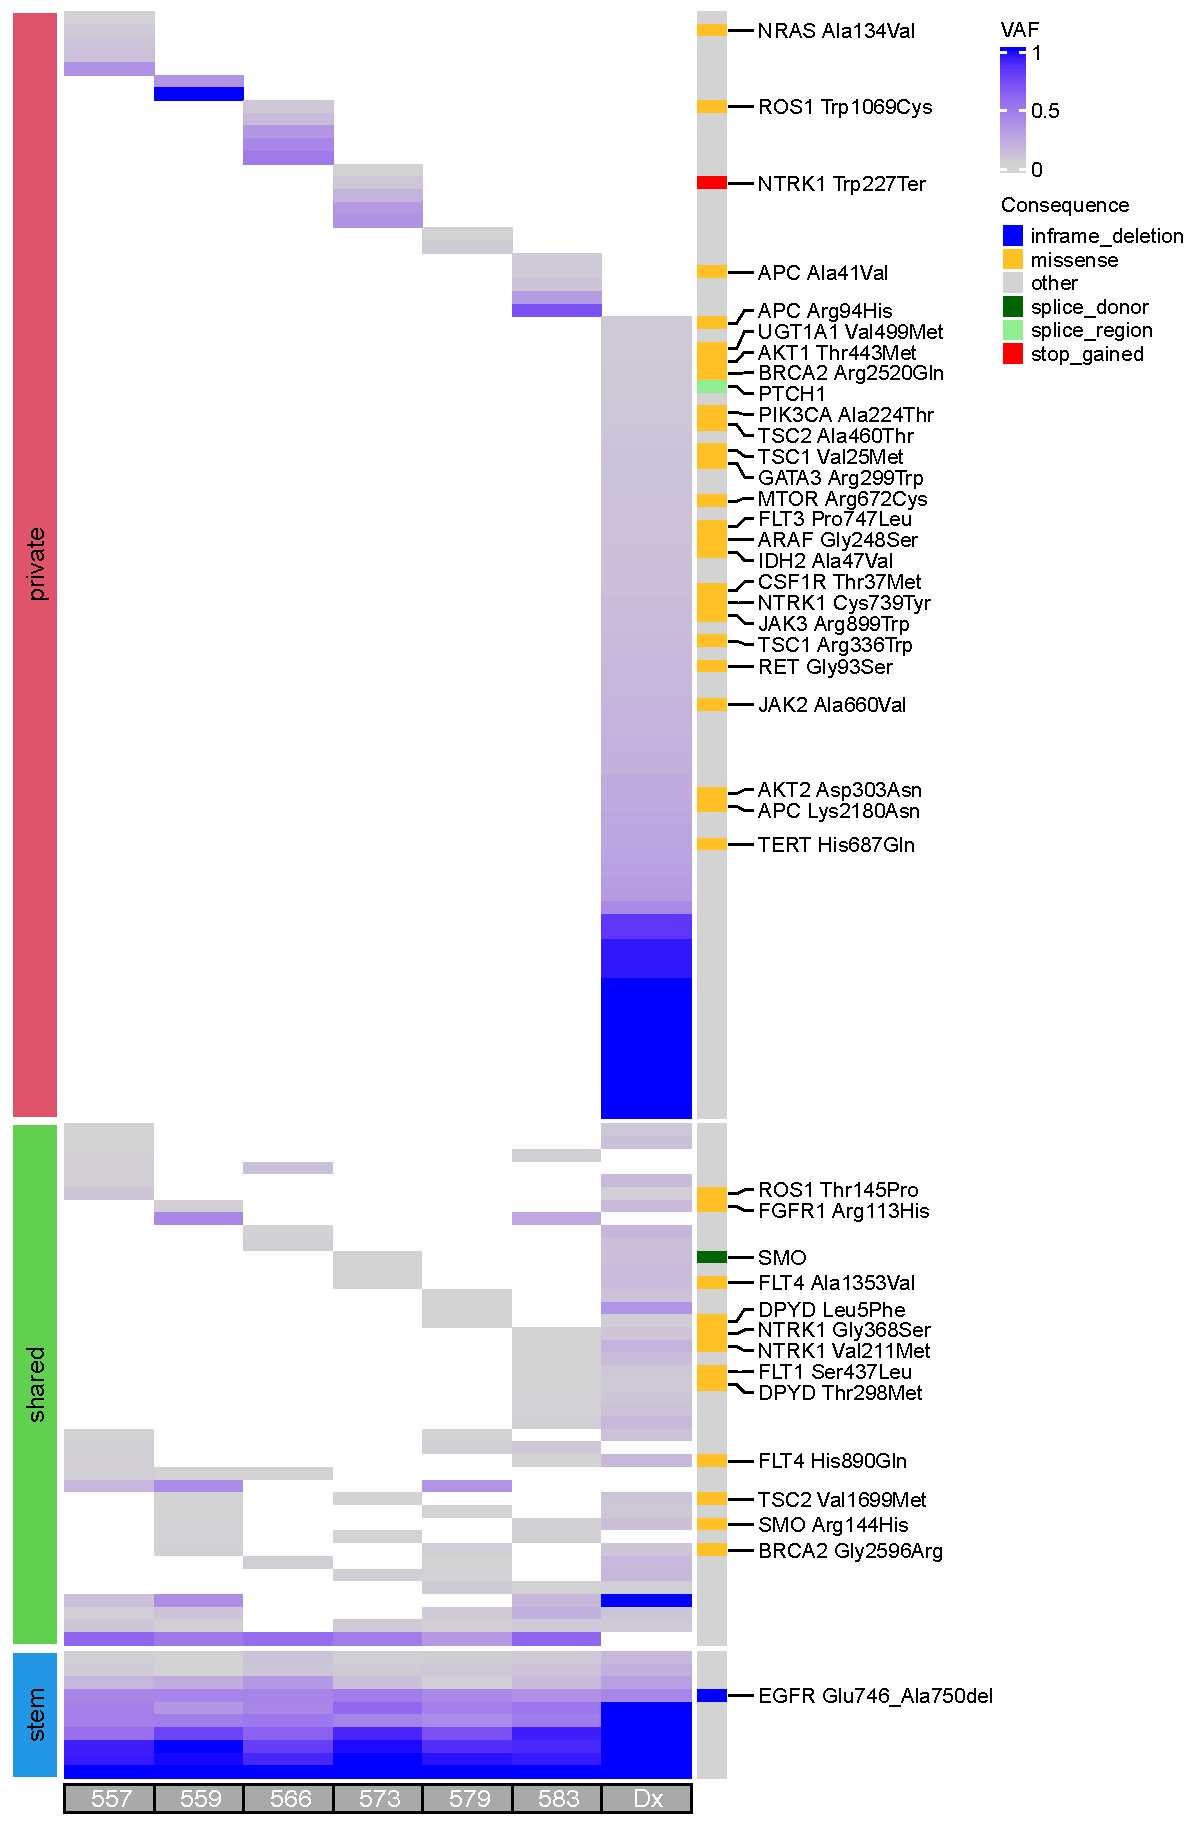
\includegraphics[width=.99\linewidth]{Figures/CASCADE/CA51/CA51varHeatmap.pdf}
\caption[Heatmap of driver gene variants in patient CA-I]{Heatmap of driver gene variants in patient CA-I: Protein altering mutations are highlighted with their HGVSp notation; non protein altering mutations are grouped as ``other``.} \label{fig:ca51heatmap}
\end{figure}



When comparing the diagnostic sample with the samples at autopsy the most striking difference was the lower overall copy number gain. The cause of this difference was the amplified minor allele in the diagnostic sample, which was almost completely absent in all autopsy samples. However, this amplification in the diagnostic sample could be rooted in the FFPE DNA damage combined with the lower purity of the sample, which in turn was used as a sign of amplification of the minor allele after purity correction through sequenza. 
The consistent feature between all samples, diagnostic and autopsy, was the loss of heterozygosity on chromosomes 2, 4, 10 through 13, and 19, with consistent copy number gains at the end of chromosome 1, 3 and 7 and all of chromosome 5 and 6.
The high amplification of chromosome 7 is consistent with the origin of the \textit{EGFR} driven primary tumour and the copy number loss of the start of chromosome 17 for all autopsy samples, but only a loss of heterozygosity in the primary sample is consistent with the genetic prerequisites for small cell transformation. (\autoref{fig:ca51.dxcircos} vs. \Autoref{fig:ca51.557circos,fig:ca51.559circos,fig:ca51.566circos,fig:ca51.573circos,fig:ca51.579circos,fig:ca51.583circos} and \autoref{tab:ca51cnv}).


\begin{figure}[p]
\centering
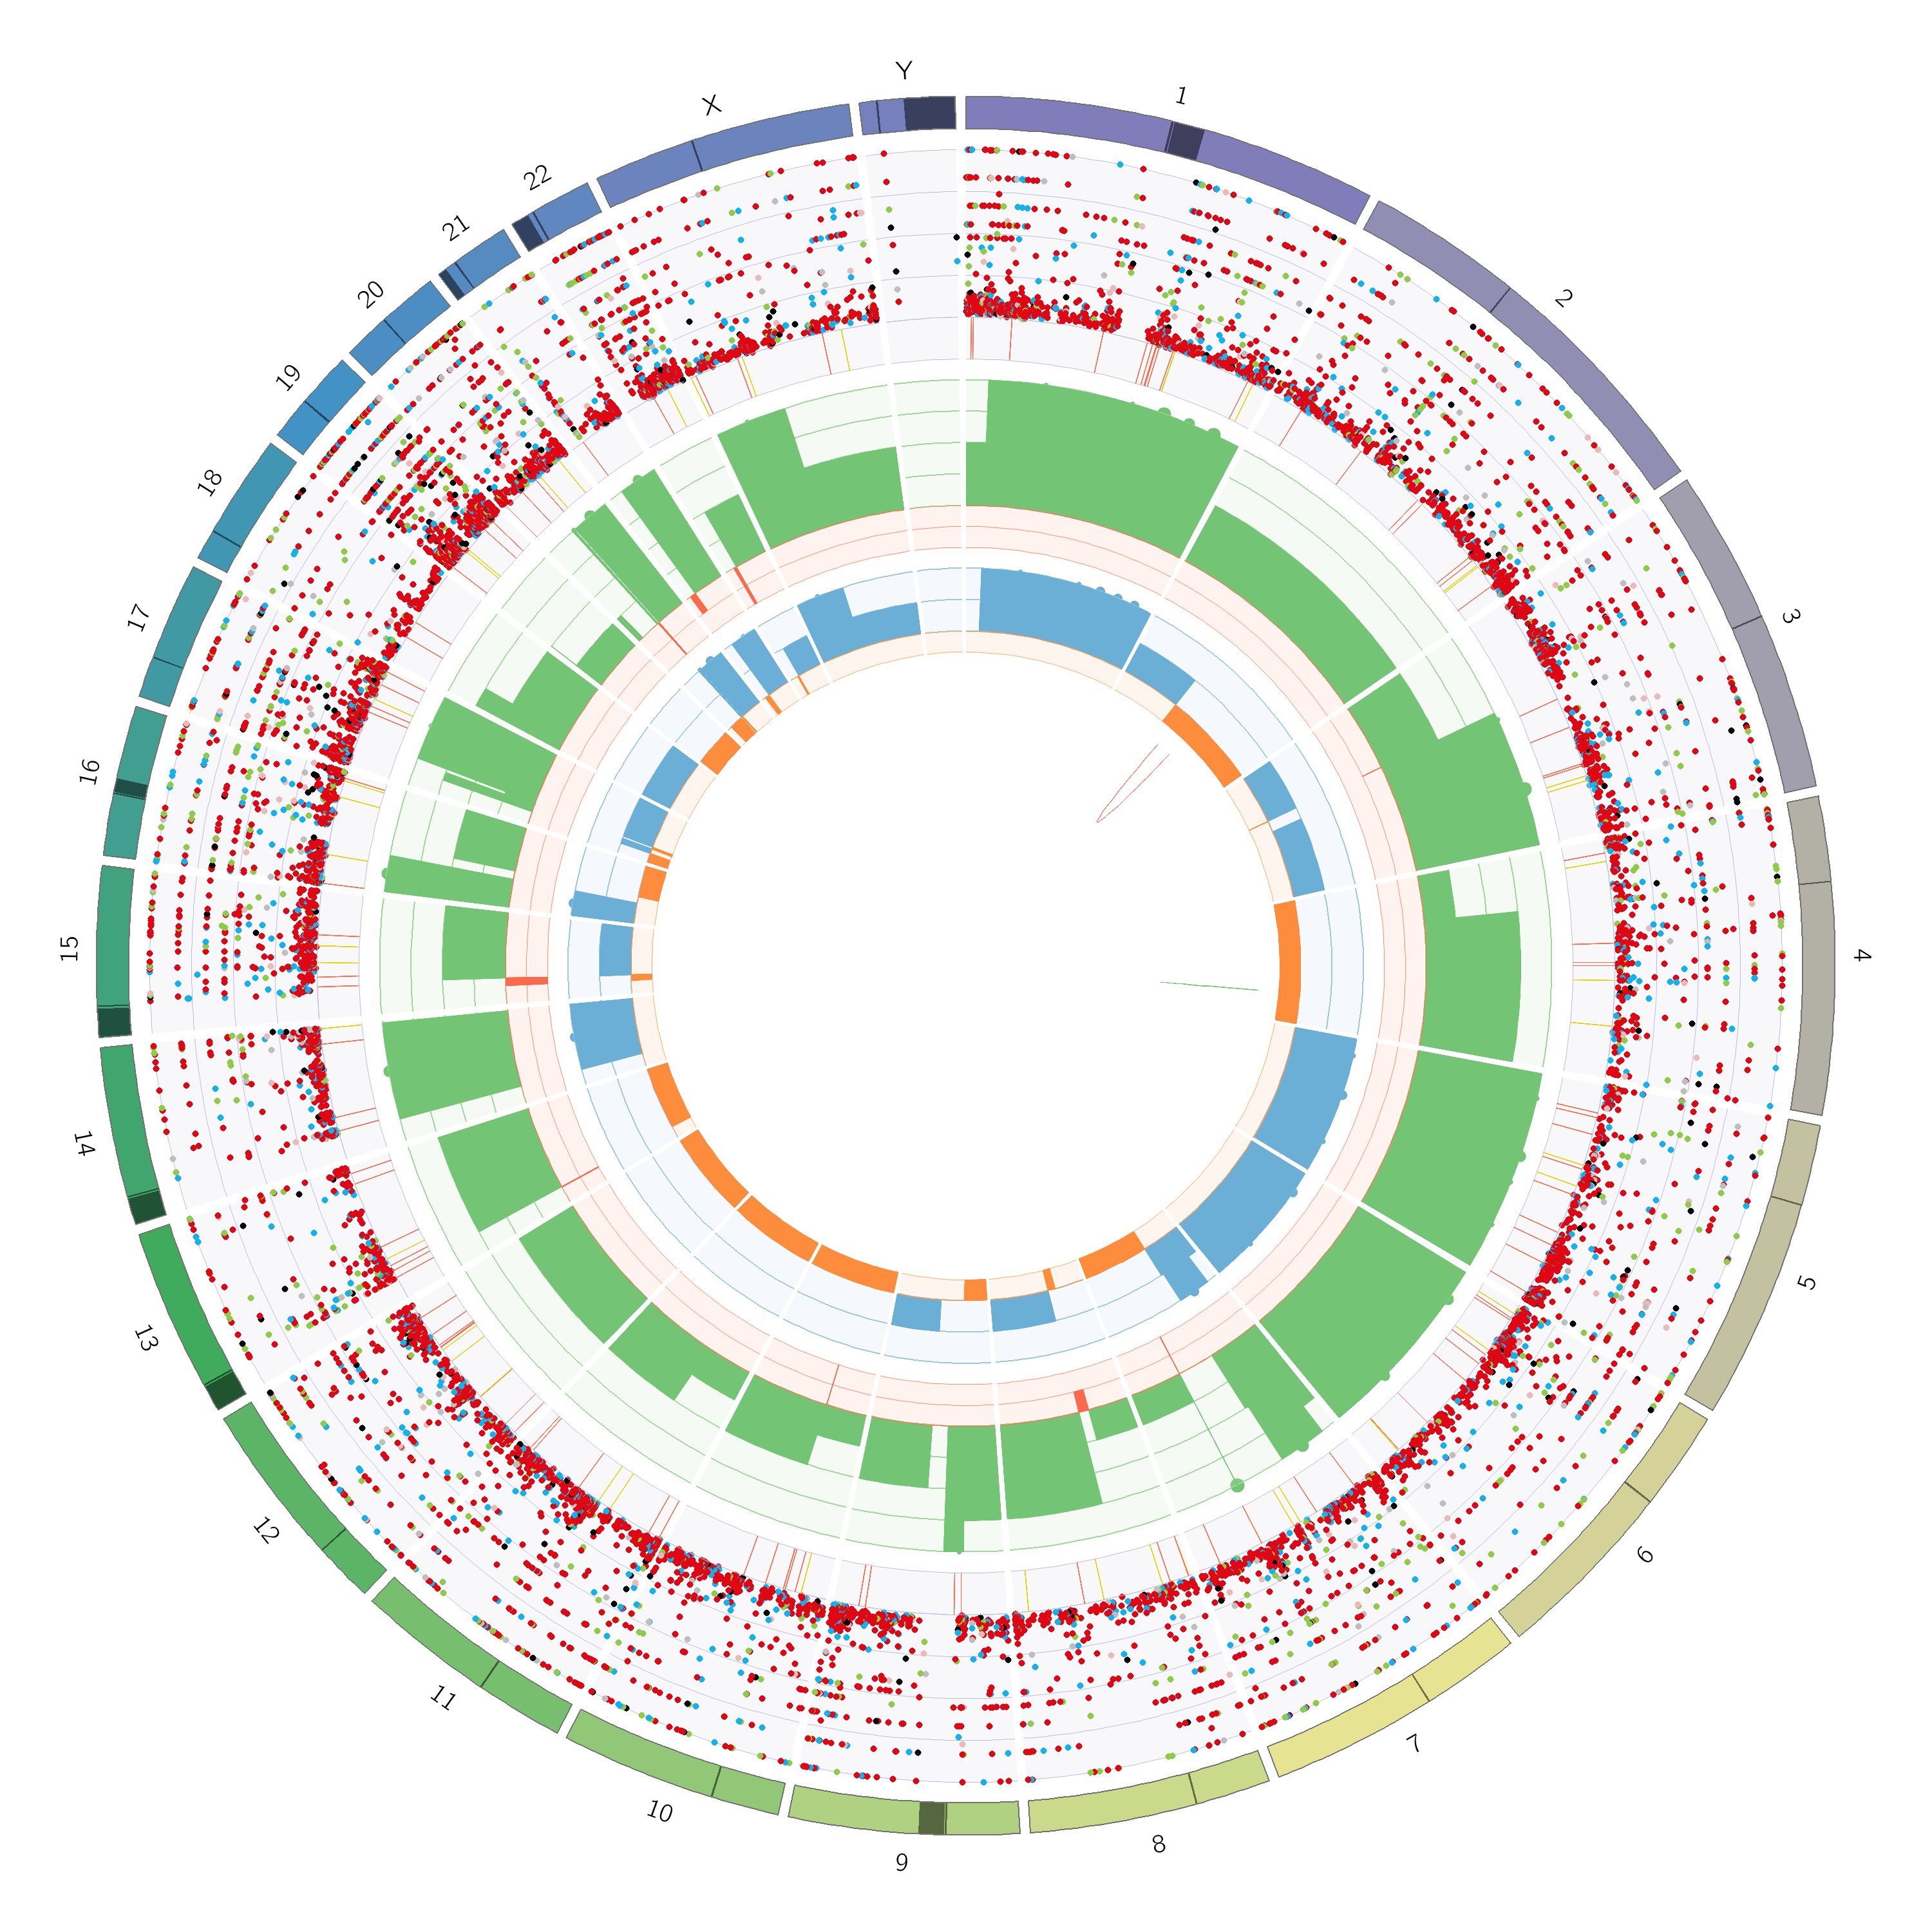
\includegraphics[width=.99\linewidth]{Figures/CASCADE/CA51/CA51-Ep12P3369.circos.png}
\caption[Circos plot of patient CA-I sample dx]{Circos plot of patient CA-I sample dx with somatic structural variants: outer first ring shows the canonical chromosomes with gaps (centromere, heterochromatin,...) highlighted as darker areas; second ring visualises all somatic SNVs corrected for tumour purity and scaled from 0 to 1, the colour representing the base change of SNV like in \protect\textcite{Alexandrov2013}; vertical lines directly under the SNVs symbolise InDels, with yellow for insertions and red for deletions; the third ring shows the total copy number alterations, with green showing a copy number gain and red a loss, dots at the outer border show a copy number greater than four; the last ring shows the minor copy number, with blue depicting a gain and orange a loss, this ring allows the detection of copy number neutral changes, like loss of heterozygosity; the center shows all structural variants: translocations in blue, deletions in red, insertions in yellow, tandem duplications in green and inversions in black.} \label{fig:ca51.dxcircos}
\end{figure}


\begin{figure}[p]
\centering
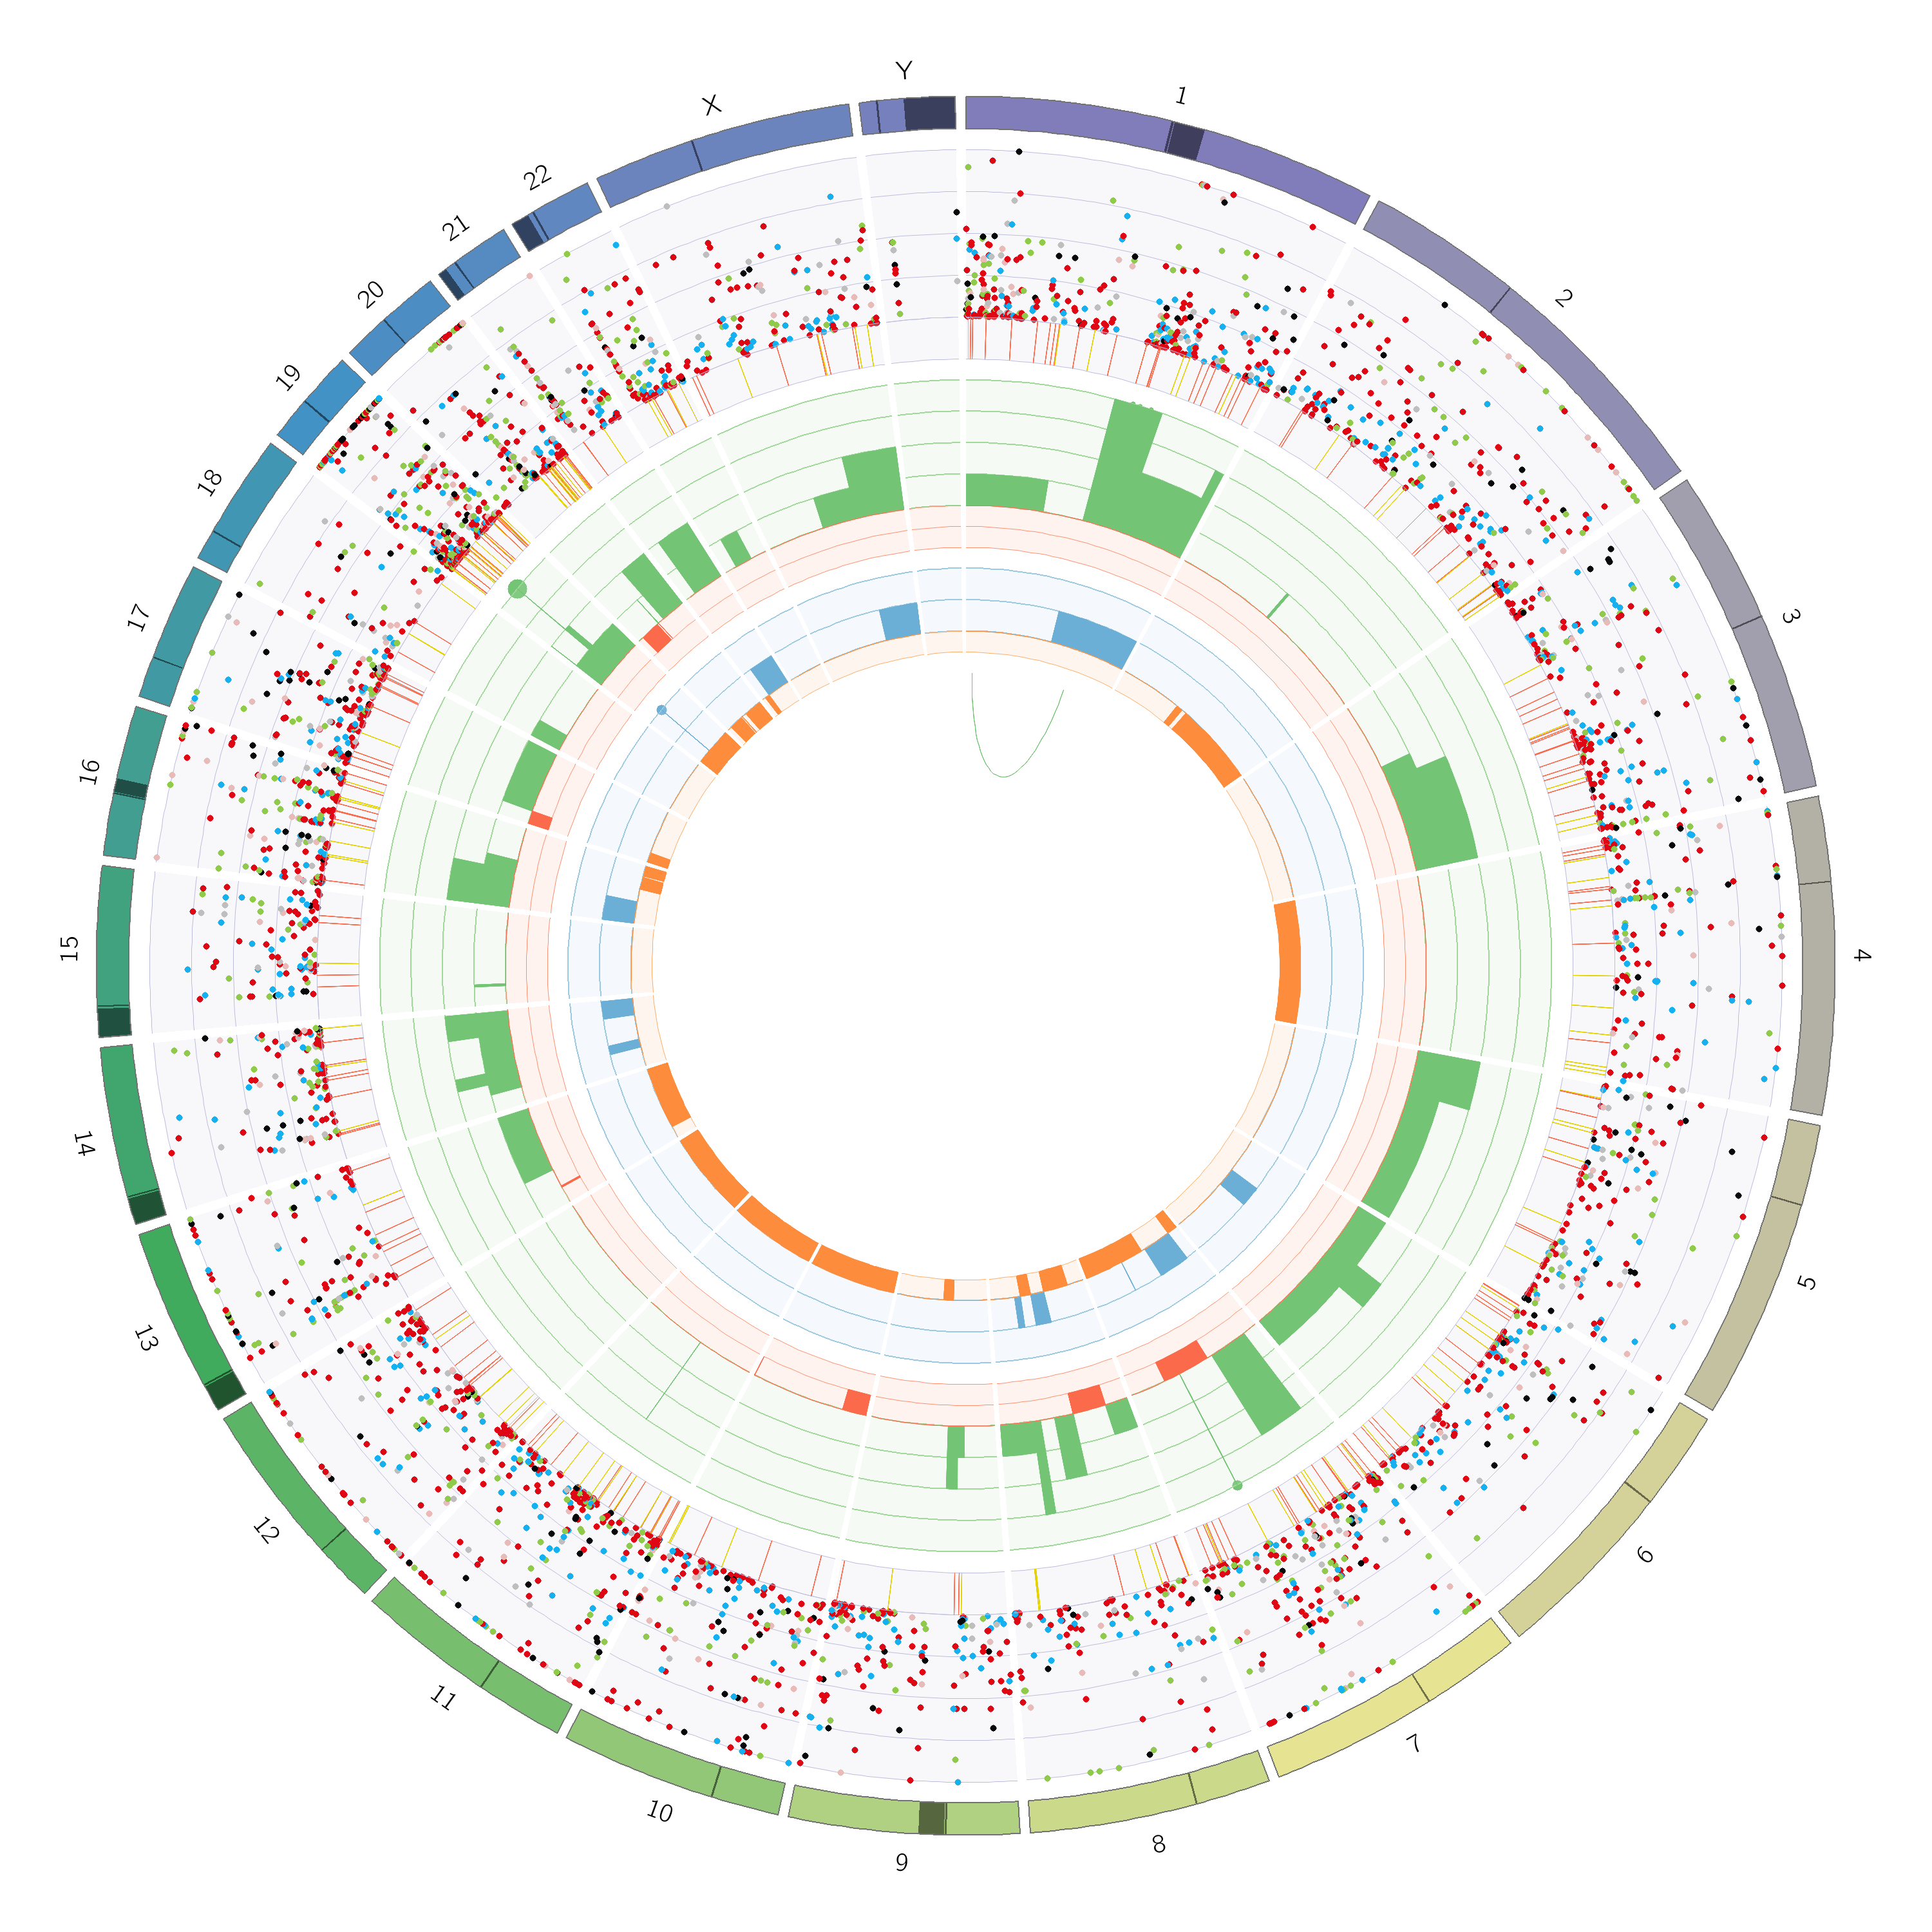
\includegraphics[width=.99\linewidth]{Figures/CASCADE/CA51/CA51-557.circos.png}
\caption[Circos plot of patient CA-I sample 557]{Circos plot of patient CA-I sample 557 with somatic structural variants: outer first ring shows the canonical chromosomes with gaps (centromere, heterochromatin,...) highlighted as darker areas; second ring visualises all somatic SNVs corrected for tumour purity and scaled from 0 to 1, the colour representing the base change of SNV like in \protect\textcite{Alexandrov2013}; vertical lines directly under the SNVs symbolise InDels, with yellow for insertions and red for deletions; the third ring shows the total copy number alterations, with green showing a copy number gain and red a loss, dots at the outer border show a copy number greater than four; the last ring shows the minor copy number, with blue depicting a gain and orange a loss, this ring allows the detection of copy number neutral changes, like loss of heterozygosity; the center shows all structural variants: translocations in blue, deletions in red, insertions in yellow, tandem duplications in green and inversions in black.} \label{fig:ca51.557circos}
\end{figure}



\begin{table}[ht]
\caption[Copy number analysis results for patient CA-I]{Copy number analysis results for patient CA-I: results are taken from the best fit result of sequenza}\label{tab:ca51cnv}
\centering
\rowcolors{2}{gray!15}{white}
\begin{tabular}{|c|c|c|c|}
\toprule
\hline
 \rowcolor{gray!50}
\textbf{Sample number} & \textbf{purity} & \textbf{ploidy} & \textbf{WG duplication}\\
\hline
 Dx  & \num{0.29} & \num{5.5} & True	\\
 557 & \num{0.93} & \num{2.6} & False \\
 559 & \num{0.96} & \num{2.6} & False \\
 566 & \num{0.69} & \num{2.7} & False \\
 573 & \num{0.94} & \num{2.6} & False \\
 579 & \num{0.95} & \num{2.6} & False \\
 583 & \num{0.95} & \num{2.6} & False \\
 \hline
\bottomrule
\end{tabular}
\end{table} 


\begin{figure}[htp]
\centering
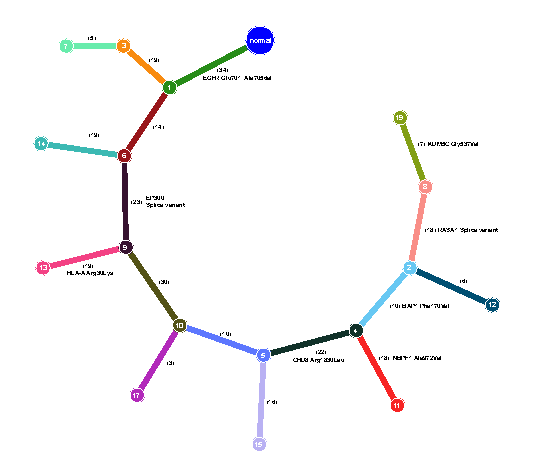
\includegraphics[width=.99\linewidth]{Figures/CASCADE/CA51/CA51.clonaltree.pdf}
\caption[Clonal evolutionary tree CA-I]{Clonal evolutionary tree of patient CA-I; Highest support tree for clustered ccf clones generated with PhylogicNDT; Support for clone is shown in parenthesis; Major driver alterations of clones were annotated; Clusters with less than 5 supporting variants were discarded; Cluster with 2000 supporting variants only present in sample Dx was discarded as FFPE artefact} \label{fig:ca51.clonalTree}
\end{figure}

Clonal deconvolution of somatic variants with PhylogicNDT revealed a linear, most likely longitudinal, development of clones adjusting to the changing treatment, with the initial clone 1 containing the exon 19 deletion and individual subclones branching off. While a HLA-A disrupting variant in cluster 13 was observed at high frequency in the diagnostic sample, it was out-competed by other clones at autopsy, and seen as transient cluster 4. Due to the small cell transformation, which correlates with down regulation of major histocompability complex (MHC) components, a direct disruption of \textit{HLA-A} was likely not necessary anymore. Some clones also were only observed in specific sites, like cluster 15 or not found at certain sites (cluster 5) which pointed to high heterogeneity of disease at autopsy (\Autoref{fig:ca51.clonalTree,fig:ca51.ccfCluster}).

These results agree with the phylogenetic reconstruction which showed initial shared somatic evolution of all sites, with strong individual evolution and limited substructure.

\begin{figure}[htp]
\centering
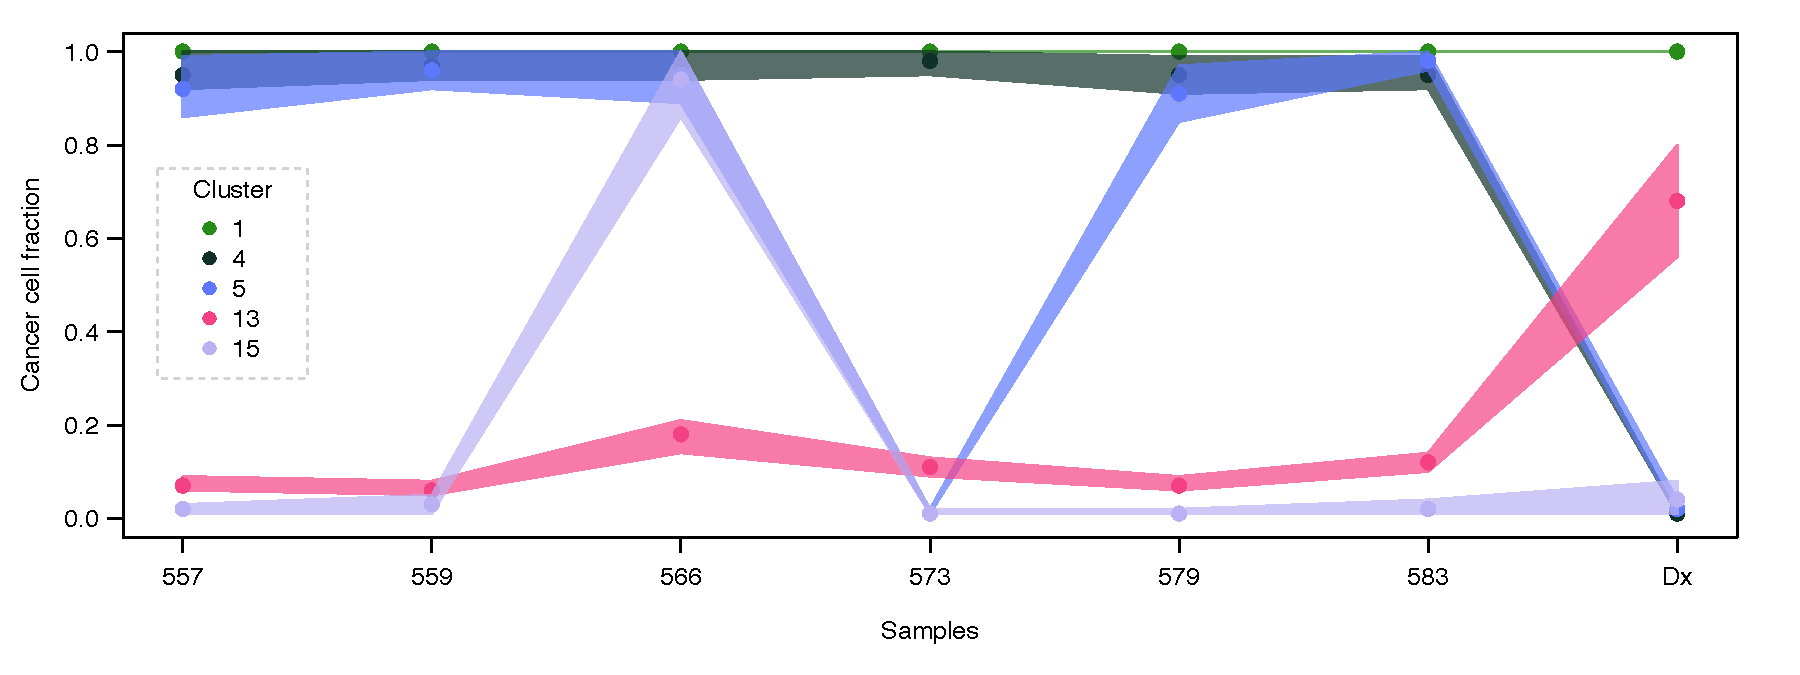
\includegraphics[width=.99\linewidth]{Figures/CASCADE/CA51/CA51.ccf_cluster.pdf}
\caption[Cancer cell fraction of mutation clusters of the clonal tree for patient CA-I]{Cancer cell fraction of mutation clusters of clonal tree for patient CA-I; transparent polygons show the 95\% confidence intervals. Clusters and cluster colours are taken from \protect\autoref{fig:ca51.clonalTree}} \label{fig:ca51.ccfCluster}
\end{figure}


%we clear all floats before we go to the next patient
\cleardoublepage

%%%%%%%%%%%%%%%%%%%%%%%%%%%%%%%%%%%%%%%%%%%%%%%%%%%%%%%%%%%%%%%%%%%%%%%%%%%%%%%%%%%%%%%
%                               Patient CA80                                          %
%%%%%%%%%%%%%%%%%%%%%%%%%%%%%%%%%%%%%%%%%%%%%%%%%%%%%%%%%%%%%%%%%%%%%%%%%%%%%%%%%%%%%%%


\subsection{Patient CA-J}
\label{cascade-sec:CA80}

Patient CA-J was a 65 year old female never smoker, who presented with moderately differentiated lung  adenocarcinoma (Stage IIIB). Molecular pathology revealed metastatic EGFR~L858R positive disease. Initial treatment with both Carboplatin/Paclitaxel and radiotherapy was halted after detection of metastatic disease with bone, left adrenal gland and bilateral lung lesions and she was changed to the tyrosine kinase inhibitor Erlotinib. Progressive pulmonary disease and subsequent left lung core biopsy showed an additional BRAF~V600E mutation. Treatment was adjusted to Carboplatin and Pemetrexed, however further disease progression was evident. The patient was finally enrolled in the EVICT trial involving treatment with the BRAF inhibitor Vemurafenib in combination with Erlotinib, which led to stable bone metastasis after one month, but ultimately led to progression of both pulmonary and bone metastases. The patient died 29 months after initial diagnosis (\autoref{fig:ca80timeline}).

\begin{figure}[ht]
\centering
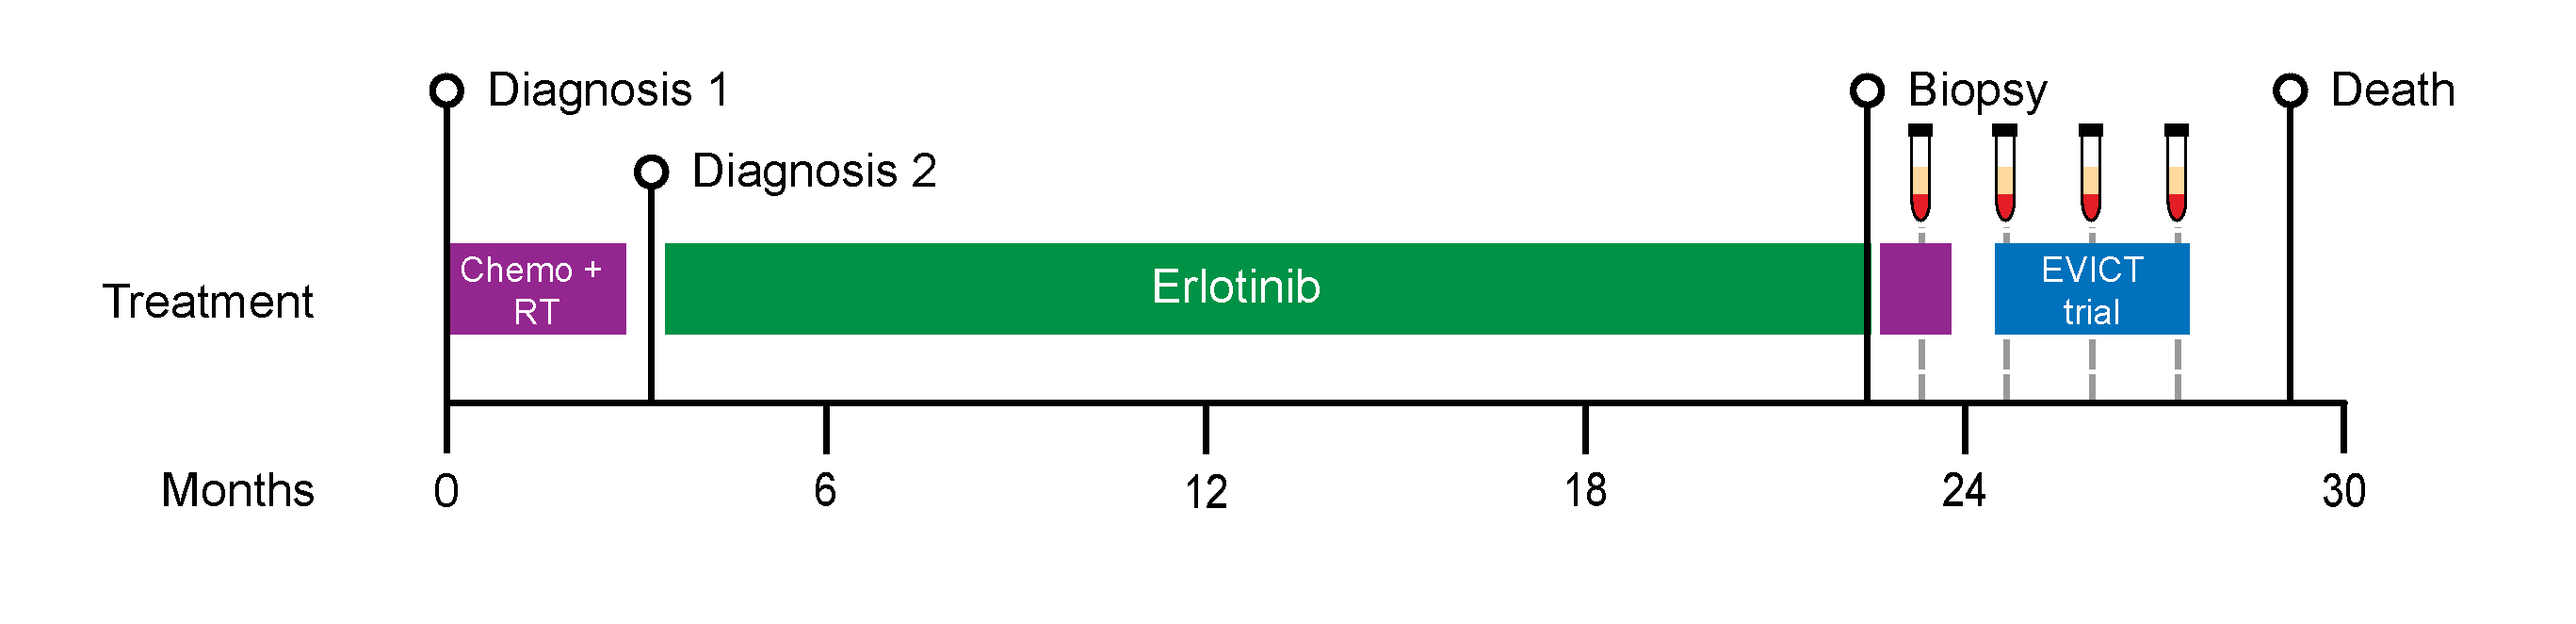
\includegraphics[width=.99\linewidth]{Figures/CASCADE/CA80/CA-J_timeline}
\caption[Timeline of patient CA-J from diagnosis until death]{Timeline of patient CA-J from diagnosis until death: Diagnostic biopsy detected EGFR~L858R positive stage IIIB lung adenocarcinoma; Second diagnosis after 3 months revealed additional brain, bone and lung metastasis with a reclassification to stage IV; Biopsy at the end of erlotinib treatment revealed additional BRAF~V600E mutation; one blood sample was taken during the second round of chemotherapy and three more during the time the patient was enrolled in the EVICT trial} \label{fig:ca80timeline}
\end{figure}

Serial plasma sampling Just before and during the enrollment in the EVICT trial allowed us to monitor the genomic landscape of the disease during treatment via specially designed ddPCR analysis. After the second round of chemotherapy a $\approx 60\%$ variant allele fraction of EGFR~L858R was found, suggesting a high ctDNA fraction. The after initial partial response to the change to Vemurafenib and Erlotinib in the EVICT trial, accompanied with a substantial drop in detectable EGFR~L858R, the patient relapsed. This progression could also be observed in the steady increase in the TP53 ``stop gained`` and BRAF~V600E mutation, which were detectable at higher levels than before the EVICT trial (\autoref{fig:ca80plasma}).

\begin{figure}[htbp]
\centering
\includegraphics[width=.99\linewidth]{Figures/CASCADE/CA80/CA80_ddPCRduringEVICT}
\caption[Blood plasma analysis of patient CA-J]{Blood plasma analysis of patient CA-J: Three putative driver mutations were analysed at four time points during during treatment. progression and partial response were assigned by clinicians based independent of ctDNA analysis; Y-axis was broken from 25-60 for visibility} \label{fig:ca80plasma}
\end{figure}


At autopsy 18 sites of disease were resected and biobanked. A representative six samples from different organs and sites were selected and WGS was performed after H\& E staining confirmed high enough tumour purity (\autoref{tab:ca80wgsSamples}, \autoref{fig:ca80schematic}). All WGS samples were analysed with the standard analysis workflow (\autoref{cascade-sec:workflow}).


\begin{figure}[ht]
\centering
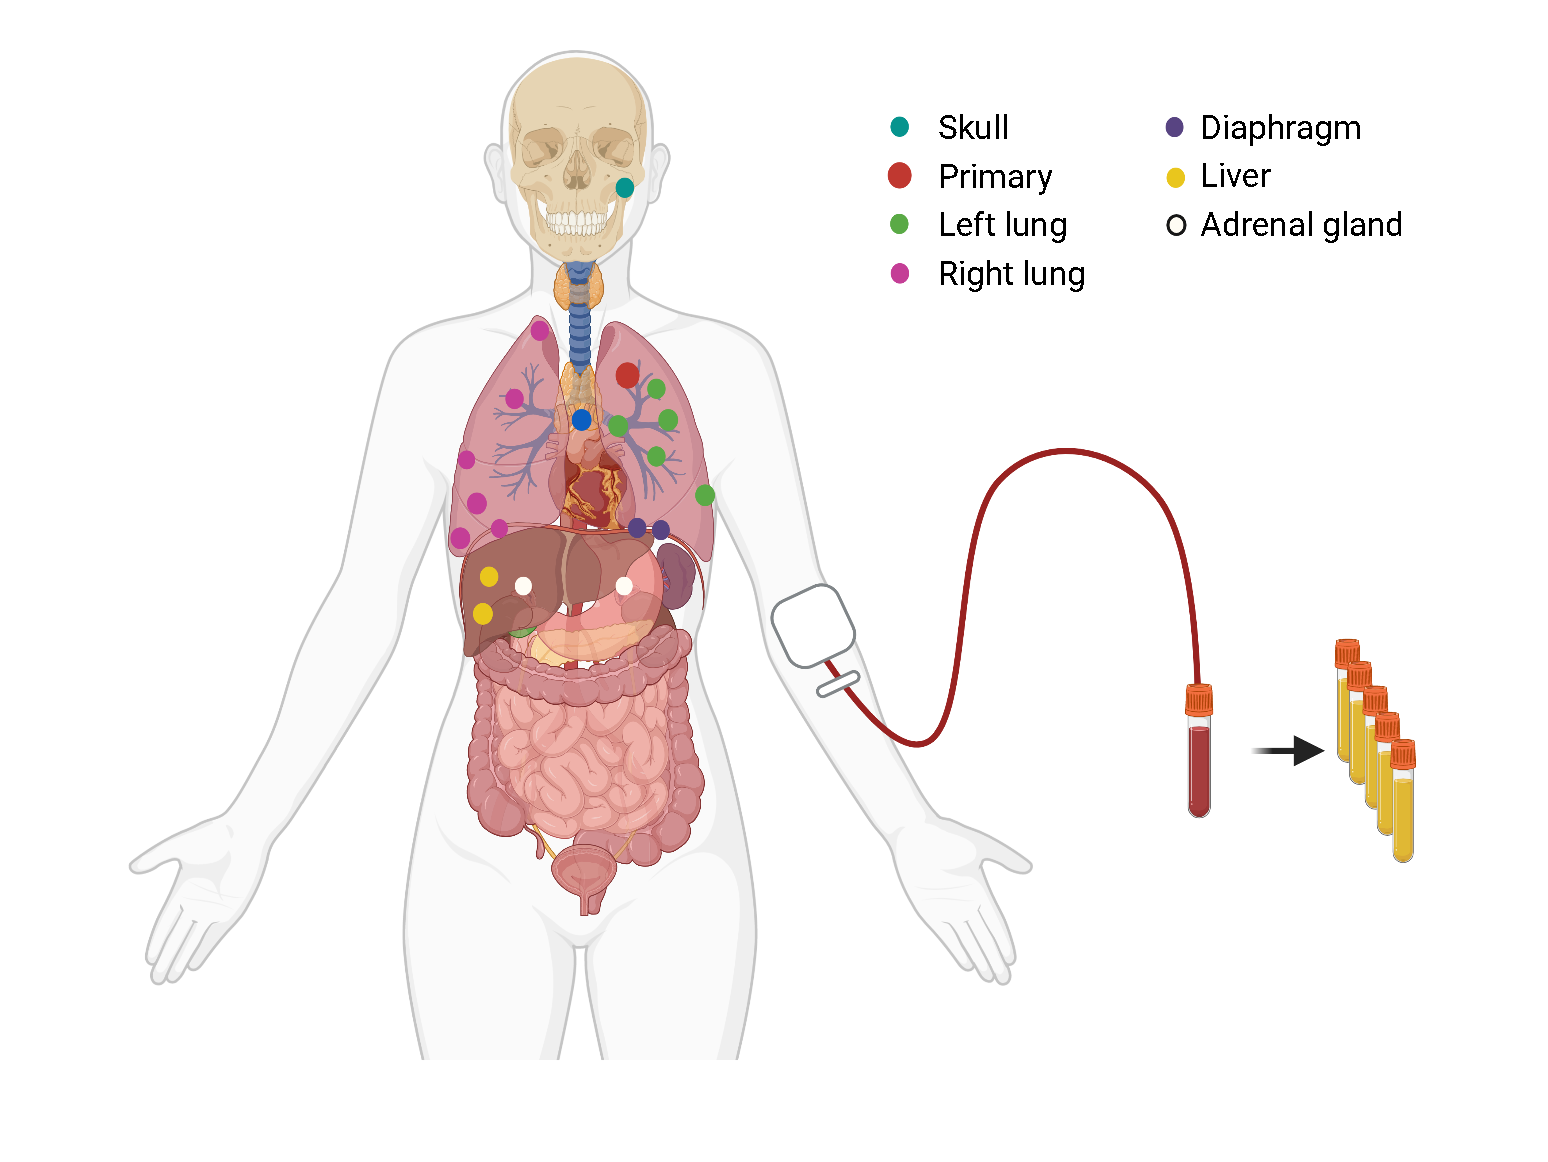
\includegraphics[width=.99\linewidth]{Figures/CASCADE/CA80/CA-J_schematic_CA80_organColours}
\caption[Schematic of analysed tumour lesions in patient CA-J]{Schematic of analysed tumour lesions in patient CA-J: Primary diagnostic sample shown in red; All 18 autopsy samples were coloured by organ they were collected from: skull (1), left lung(5), right lung (6), diaphragm (2), liver(2), adrenal gland (2); Additionally to the post mortem blood sample, four serial blood samples were taken (\protect\autoref{fig:ca80timeline})} \label{fig:ca80schematic}
\end{figure}

\begin{table}[ht]
\caption[Autopsy samples sequenced for patient CA-J]{Autopsy samples sequenced for patient CA-J: Sample number is the internal sample collection during CASCADE autopsy, the organ of the sample, the fraction of tumour cells from H\& E stain and the pathology of the tumour sample. Dx: diagnostic sample}\label{tab:ca80wgsSamples}
\centering
\rowcolors{2}{gray!15}{white}
\begin{tabular}{|c|c|c|c|c|}
\toprule
\hline
 \rowcolor{gray!50}
\textbf{Sample number} & \textbf{Organ} & \textbf{H\&E} & \textbf{Type}\\
\hline
 Dx & left lung core & - & \cellcolor{white} \\
 2 & adrenal gland & 0.5 & \cellcolor{white} \\
 20 & right lower lung & 0.7 & \cellcolor{white} \\
 24 & left upper lung & 0.9 & \cellcolor{white} \\
 28 & left middle lung & 0.5 & \cellcolor{white} \\
 32 & right upper lung & 0.5 & \cellcolor{white} \\
 42 & base of skull & 0.4 & \cellcolor{white}\multirow{-7}{*}{adenocarcinoma} \\
 \hline
\bottomrule
\end{tabular}
\end{table} 

Somatic variant calling revealed heterogeneity of resistance and driver mutations. While the initial driver variant EGFR~L858R was present in all autopsy samples, sample 2 presented with an allele frequency of 0.13 with clonal presence in all other sample. The secondary BRAF~V600E mutation, which was detected in the progression biopsy 22 months after diagnosis, was not present in sample 2 and only at low allele frequency (0.13) in sample 28. Only sample 32 showed the \textit{BRAF} mutation at 100\% VAF. While the absence in sample 2 could be explained by the overall low tumour purity of the sample, both 24 and 42 had a higher than 50\% estimated tumour purity (\autoref{tab:ca80cnv}) and showed a lower VAF, therefore suggesting a lesser involvement of the mutation in resistance.

Additionally to the \textit{BRAF} mutation, some sites (20, 24, 32, and 42) developed a ``stop gained`` mutation in \textit{TP53} (TP53~G38Ter) at 100\% VAF. While both the \textit{BRAF} and \textit{TP53} mutations were present at similar allele fractions in the diagnostic sample (Dx) suggesting a clonal structure, the \textit{TP53} variant was more prevalent at autopsy in multiple samples. So while \textit{BRAF} and \textit{TP53} mutations were correlated in the diagnostic sample, the \textit{TP53} ``stop gained`` developed independently.
Sample 28 in spite of showing traces of BRAF~V600E did not develop a \textit{TP53} mutation and sample 2, which did not contain a \textit{BRAF} change instead exhibited two different additional putative driver events (FLT4~V1097M and KEAP1~Q282H) which were not observed in any other sample. 
Finally, Sample 32 also contained a subclonal KRAS~L5Q mutation in addition to both \textit{BRAF} and \textit{TP53} mutations (\autoref{fig:ca80heatmap}). 

The emergence of the \textit{TP53} mutations was related to expansion of samples 20, 24, 32, and 42 differentiating them from the adrenal gland (2) and the original site of disease. This very early split and seeding and the low abundance of the putative \textit{EGFR} driver mutation suggests at very different disease trajectories (\autoref{fig:ca80phylo}). 

\begin{figure}[htp]
	\centering
	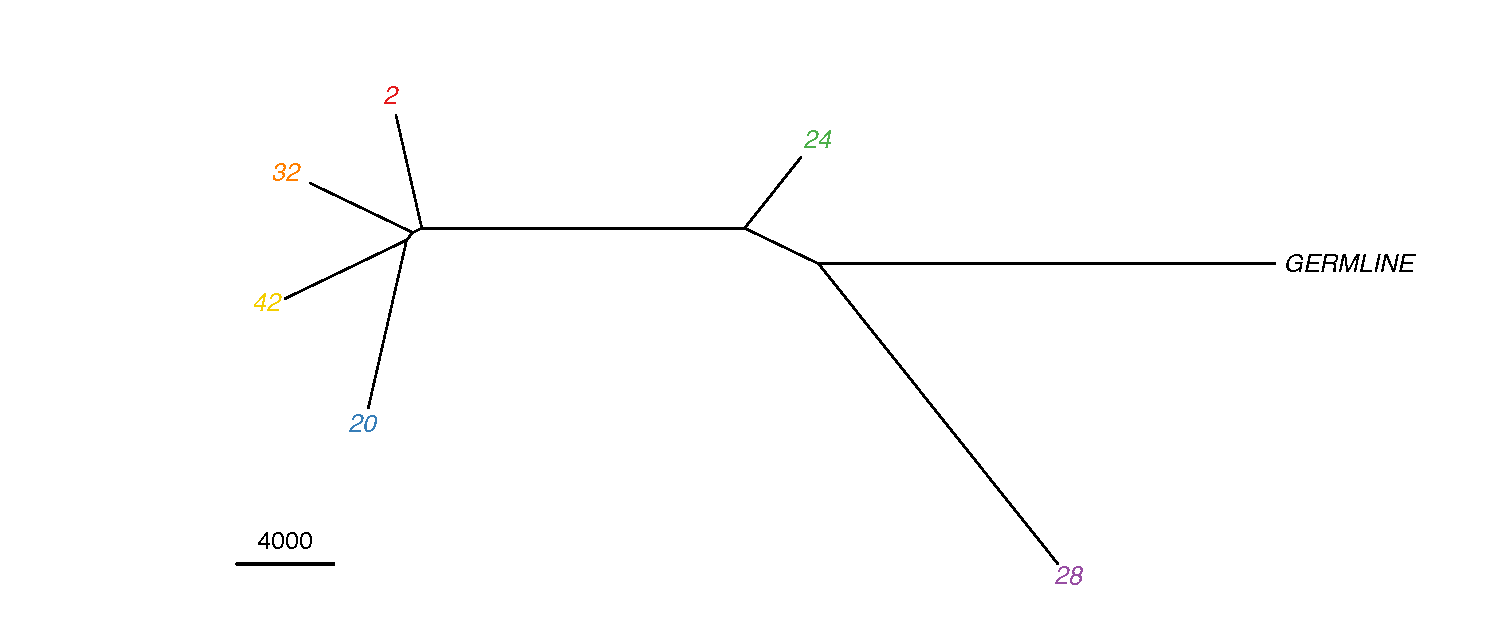
\includegraphics[width=.99\linewidth]{Figures/CASCADE/CA80/CA80phylo.pdf}
	\caption[Phylogeny of autopsy samples from patient CA-J]{Phylogeny of autopsy samples from patient CA-J; reconstructed with all somatic SNVs and InDels. Ruler symbolises 4000 variants difference.} \label{fig:ca80phylo}
\end{figure}


\begin{figure}[htp]
\centering
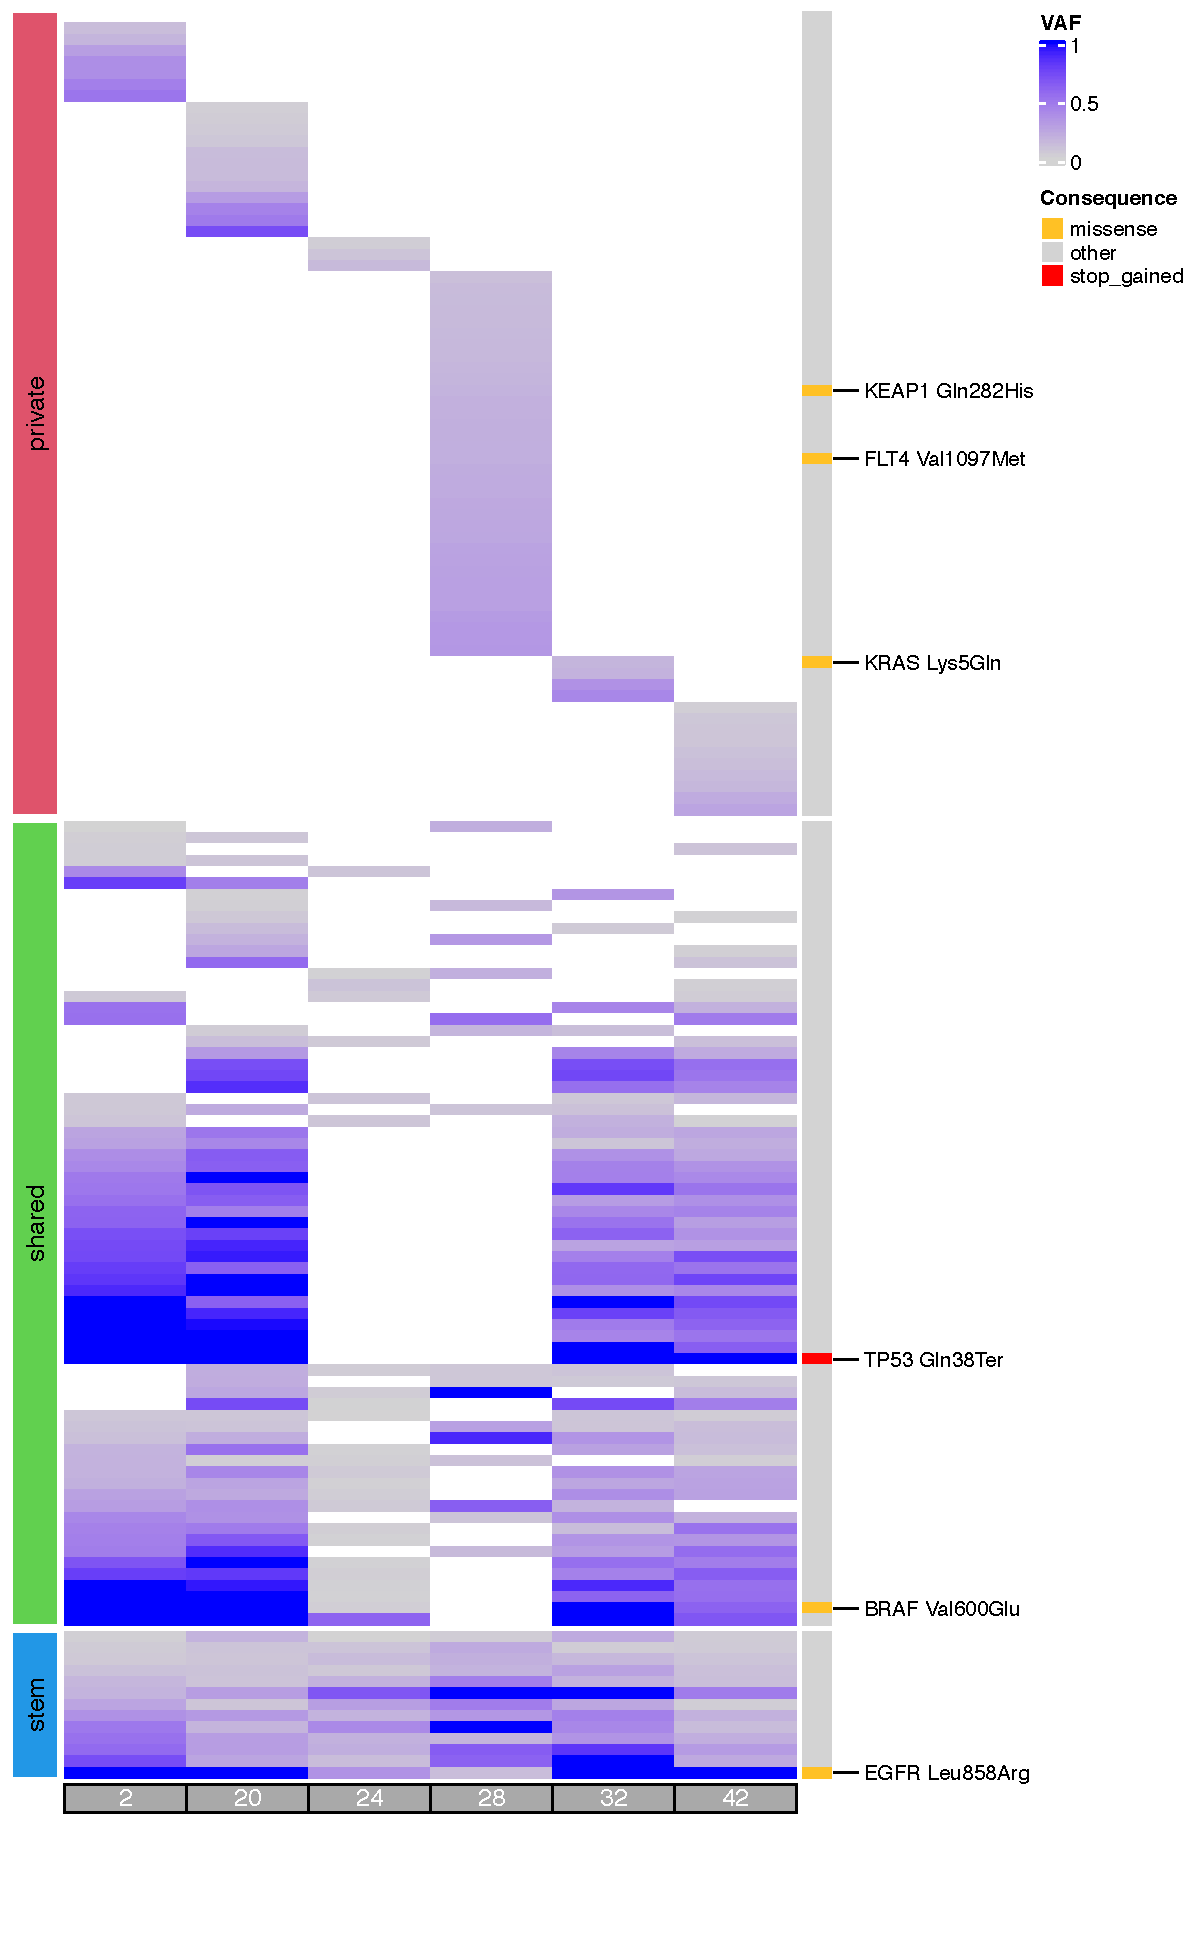
\includegraphics[width=.99\linewidth]{Figures/CASCADE/CA80/CA80varHeatmap.pdf}
\caption[Heatmap of driver gene variants in patient CA-J]{Heatmap of driver gene variants in patient CA-J: Protein altering mutations are highlighted with their HGVSp notation; non protein altering mutations are grouped as ``other``.} \label{fig:ca80heatmap}
\end{figure}



Similar to the short variants, there were some structural variants present in all samples. The inversions on chromosome 12 as well as the co-located break and fusion with the start of chromosome 5 could be observed in all samples, even those with very low tumour purity, but the inversions and fusions of chromosome 7, 8, 9, and 11 could only be seen in the higher purity samples 20, 24, 32, and 42 and most were subclonal, as they only had a median allele frequency of 14.3\% (min: 10.3\%, max: 99.7\%) in all samples.
While multiple samples exhibited gene fusions with lung cancer driver and resistance genes like \textit{BRAF}, \textit{FGFR1} and \textit{GNAS} these fusions were only present at subclonal levels $\leq 10\%$.

All samples apart from sample 2 showed whole genome duplication and high polyclonality, which suggests that in addition to the heterogeneity observed through short and structural variants, there was an additional level of heterogeneity of copy number alterations. The lower purity of sample 2 might have been a confounding factor, however both sample 28 and 32 showed lower purities, but a much higher polyclonality and genome duplication. While sample 2 had several minor focal amplifications in \textit{PMS2}, \textit{STK11} and \textit{GADD45B}, no major copy number amplification was found. All other samples showed amplifications in \textit{KRAS} (min: 2.9, max: 5.0, median: 4.6), \textit{CDK4} (min: 3.2, max: 24.4, median: 21.7) and \textit{BRAF} (min: 2.1, max: 6.0, median: 3.9) in addition to the highly amplified \textit{EGFR} (min: 10.6, max: 266.7, median: 197.4) and \textit{MET} (min: 4.2, max: 6.3, median: 4.6) locus. Both \textit{EGFR} and \textit{MET} copy number gain most likely were the resistance mechanism to the initial treatment with the tyrosine kinase inhibitor Erlotinib. (\Autoref{fig:ca80.2circos,fig:ca80.20circos,fig:ca80.24circos,fig:ca80.28circos,fig:ca80.32circos,fig:ca80.42circos} , \autoref{tab:ca80cnv}).


\begin{figure}[htp]
\centering
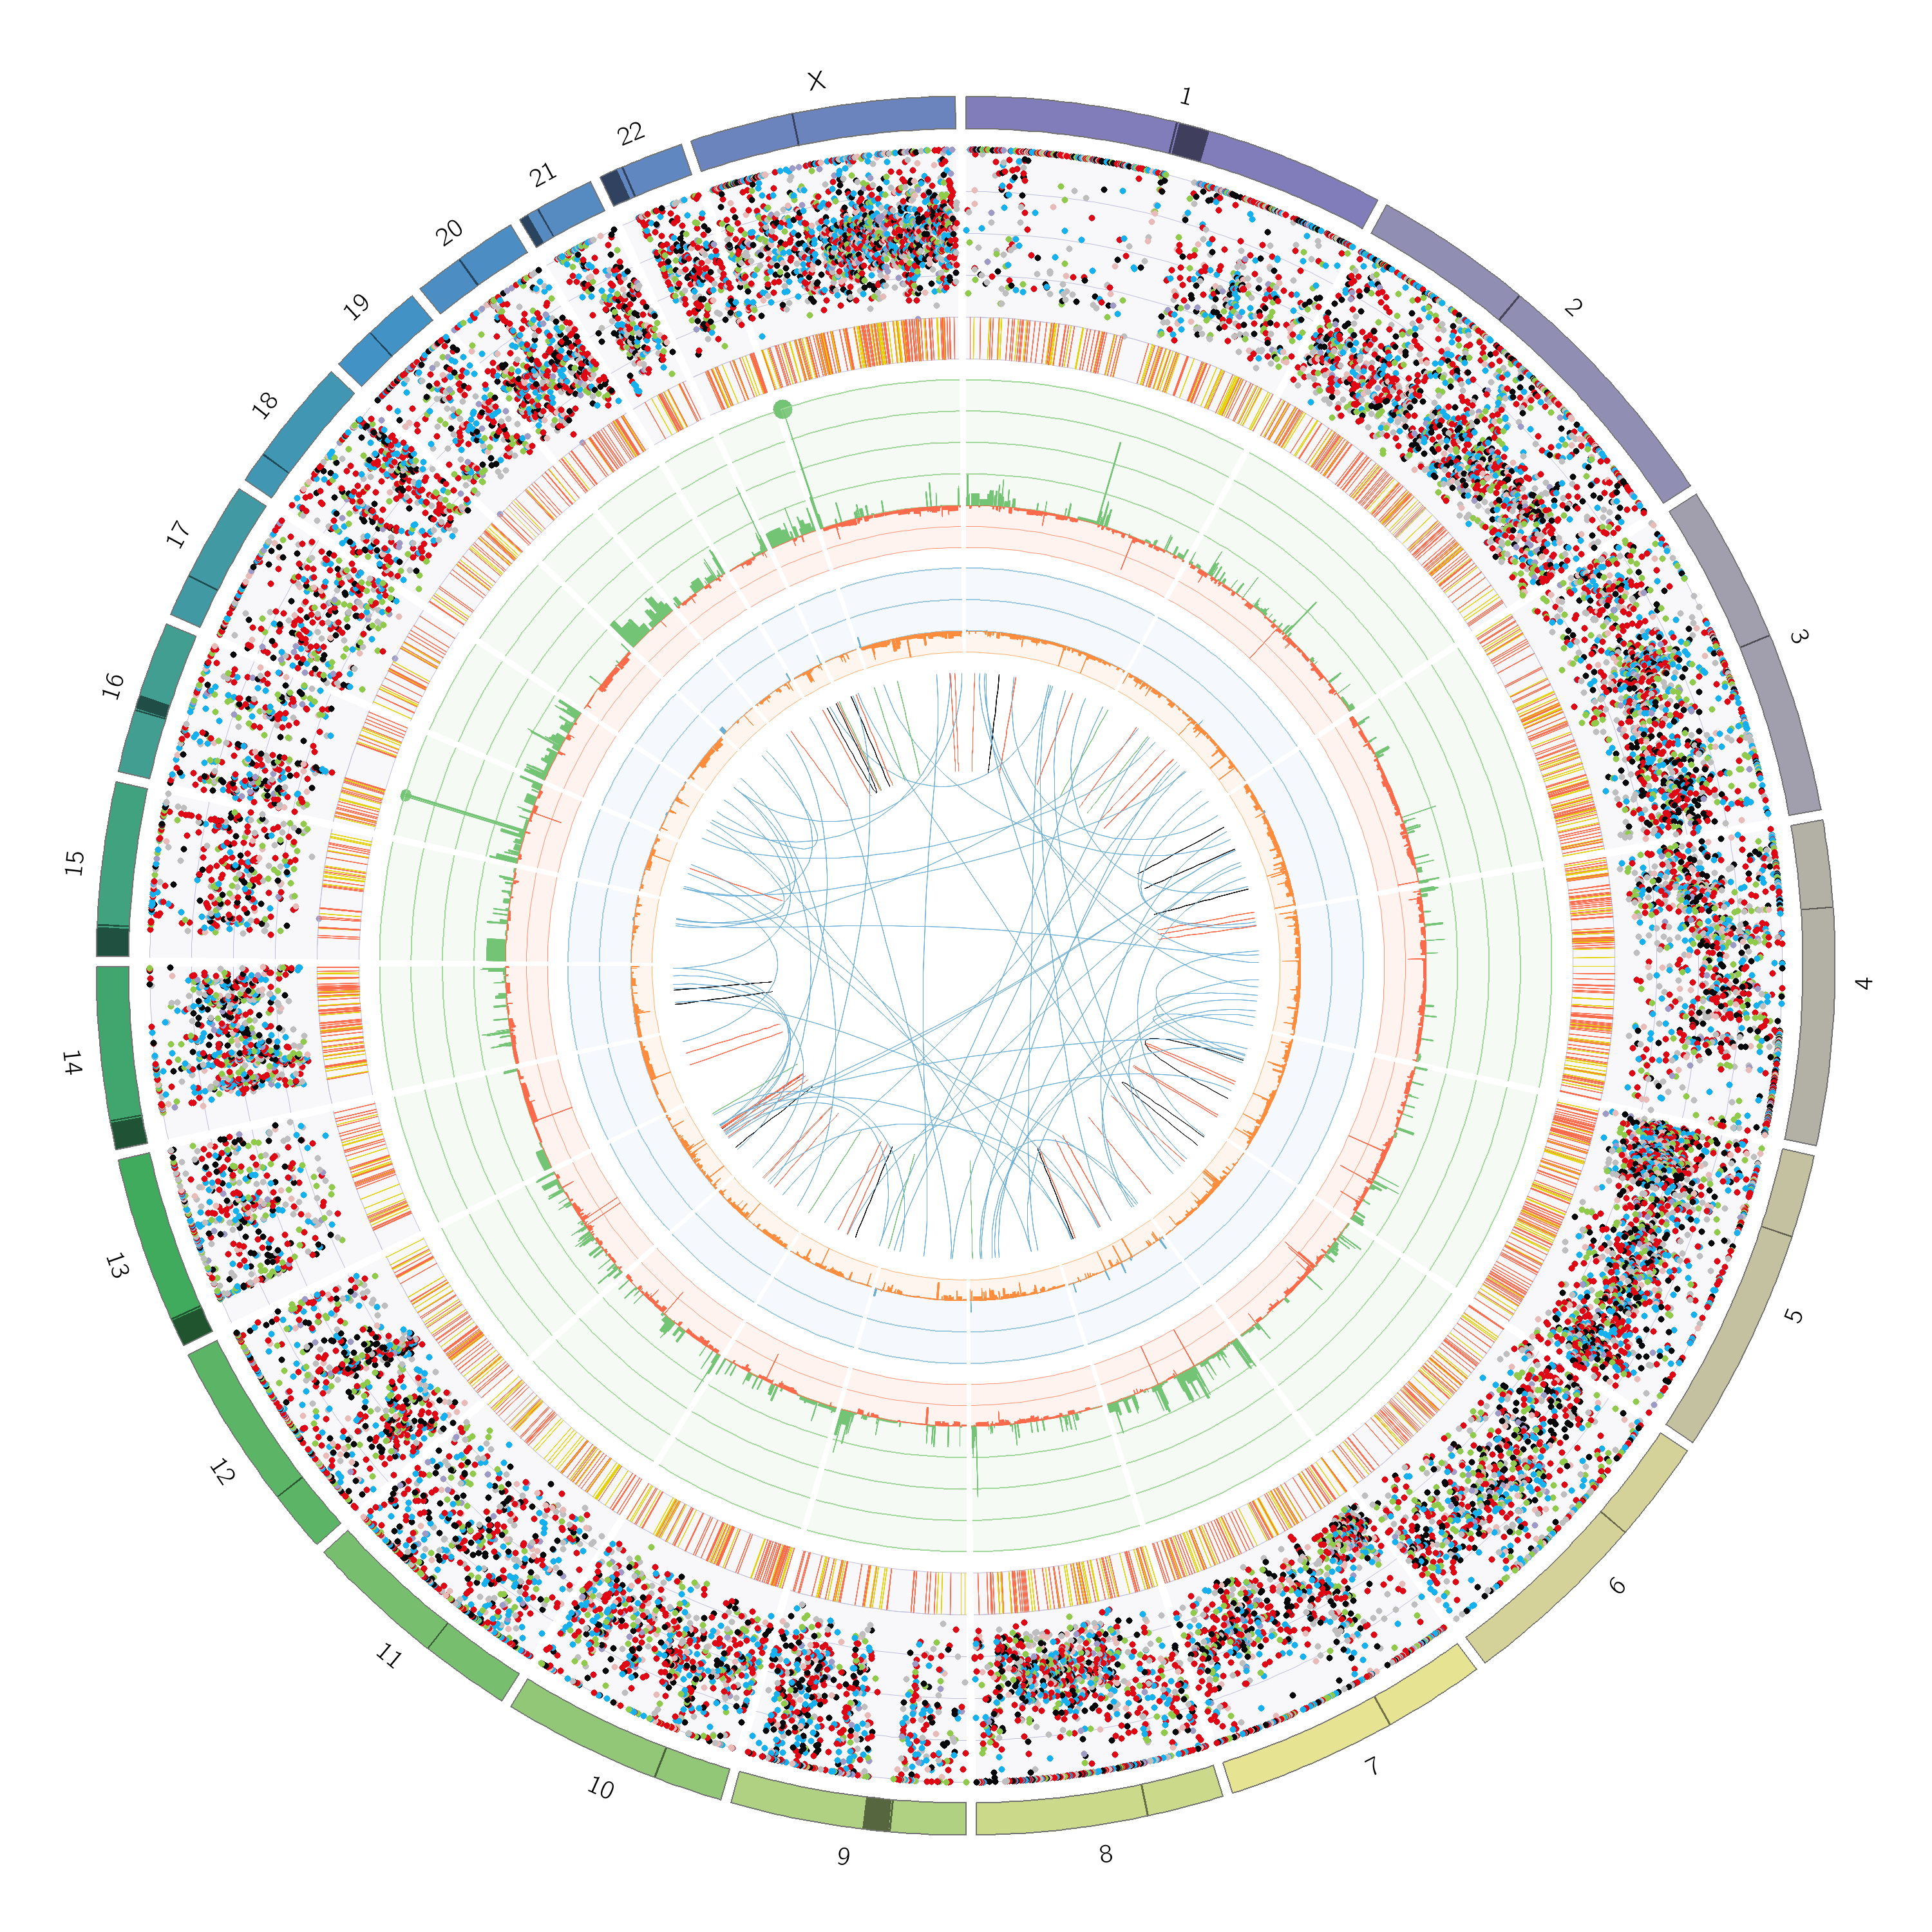
\includegraphics[width=.99\linewidth]{Figures/CASCADE/CA80/CA80-2.circos.png}
\caption[Circos plot of patient CA-J sample 2]{Circos plot of patient CA-J sample 2 with somatic structural variants with allele frequency $\geq 0.1$: outer first ring shows the canonical chromosomes with gaps (centromere, heterochromatin,...) highlighted as darker areas; second ring visualises all somatic SNVs corrected for tumour purity and scaled from 0 to 1, the colour representing the base change of SNV like in \protect\textcite{Alexandrov2013}; vertical lines directly under the SNVs symbolise InDels, with yellow for insertions and red for deletions; the third ring shows the total copy number alterations, with green showing a copy number gain and red a loss, dots at the outer border show a copy number greater than four; the last ring shows the minor copy number, with blue depicting a gain and orange a loss, this ring allows the detection of copy number neutral changes, like loss of heterozygosity; the center shows all structural variants: translocations in blue, deletions in red, insertions in yellow, tandem duplications in green and inversions in black.} \label{fig:ca80.2circos}
\end{figure}

\begin{figure}[htp]
\centering
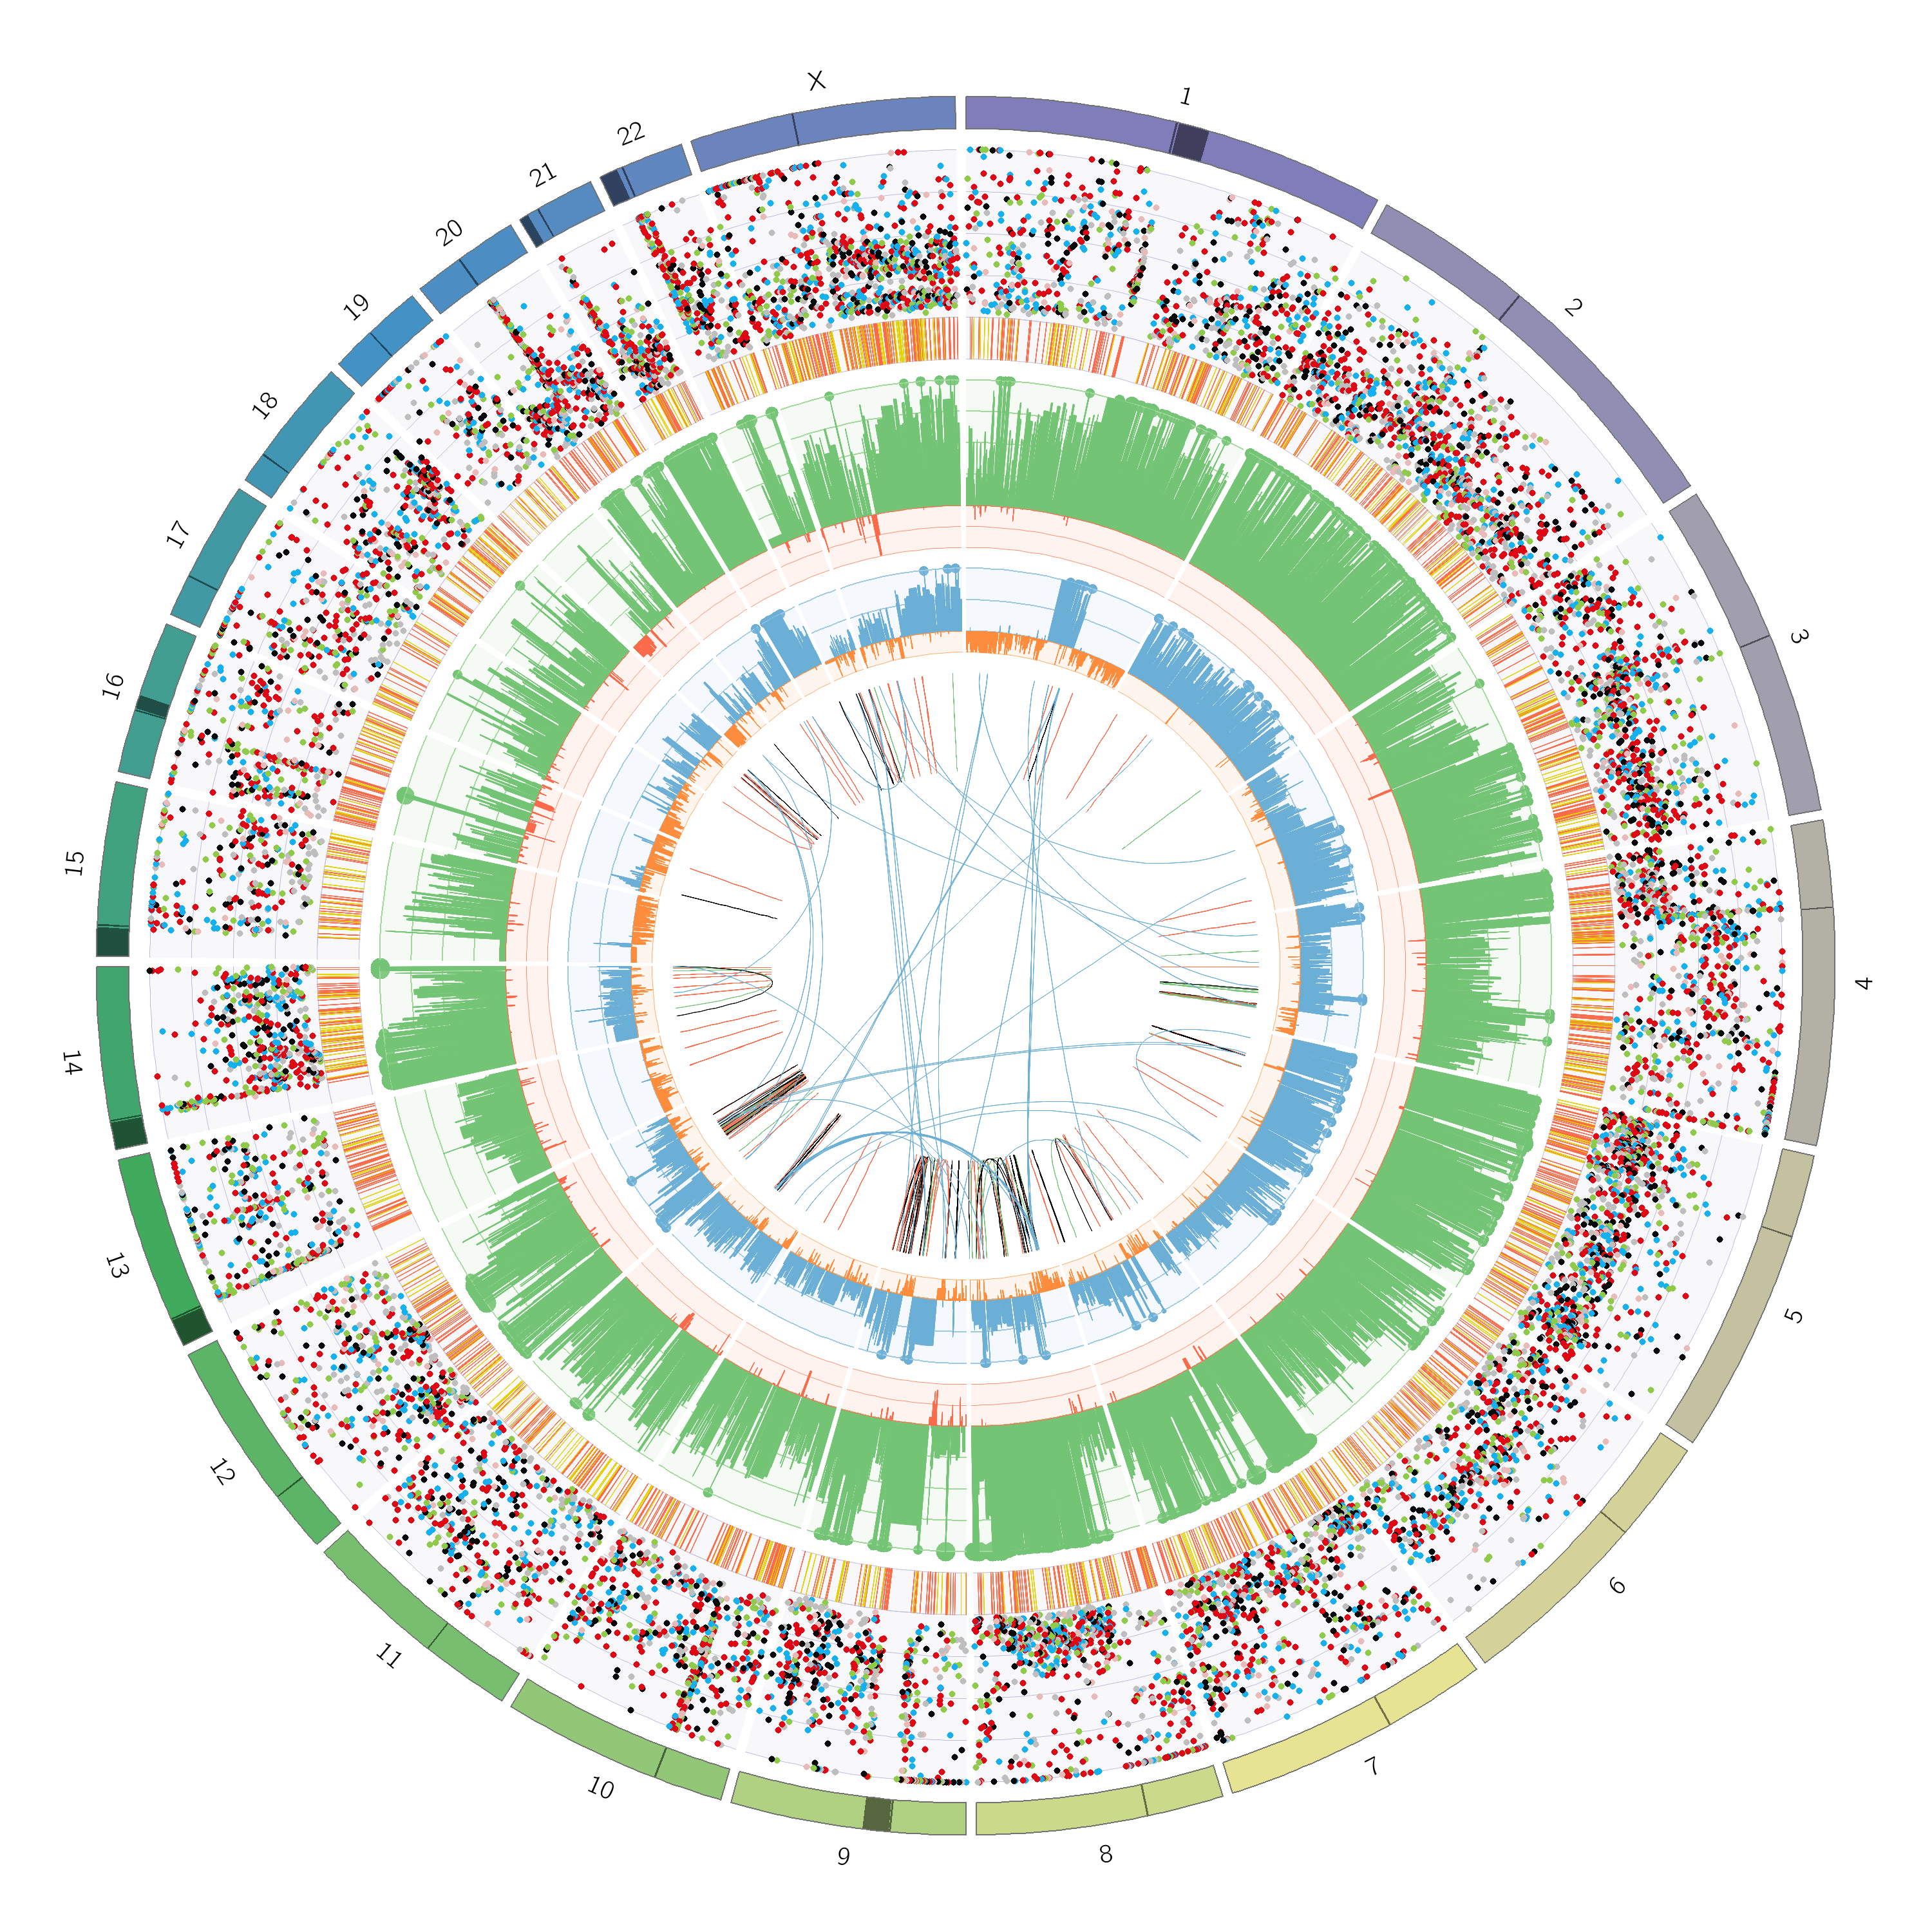
\includegraphics[width=.99\linewidth]{Figures/CASCADE/CA80/CA80-20.circos.png}
\caption[Circos plot of patient CA-J sample 20]{Circos plot of patient CA-J sample 20 with somatic structural variants with allele frequency $\geq 0.1$: outer first ring shows the canonical chromosomes with gaps (centromere, heterochromatin,...) highlighted as darker areas; second ring visualises all somatic SNVs corrected for tumour purity and scaled from 0 to 1, the colour representing the base change of SNV like in \protect\textcite{Alexandrov2013}; vertical lines directly under the SNVs symbolise InDels, with yellow for insertions and red for deletions; the third ring shows the total copy number alterations, with green showing a copy number gain and red a loss, dots at the outer border show a copy number greater than four; the last ring shows the minor copy number, with blue depicting a gain and orange a loss, this ring allows the detection of copy number neutral changes, like loss of heterozygosity; the center shows all structural variants: translocations in blue, deletions in red, insertions in yellow, tandem duplications in green and inversions in black.} \label{fig:ca80.20circos}
\end{figure}


\begin{table}[ht]
\caption[Copy number analysis results for patient CA-J]{Copy number analysis results for patient CA-J: results are taken from the best fit result of PURPLE; WG: whole genome}\label{tab:ca80cnv}
\centering
\rowcolors{2}{gray!15}{white}
\begin{tabular}{|c|c|c|c|c|}
\toprule
\hline
 \rowcolor{gray!50}
\textbf{Sample number} & \textbf{purity} & \textbf{ploidy} & \textbf{polyclonal \%} & \textbf{WG duplication}\\
\hline
 2  & \num{0.16} & \num{2.18} & \num{22.53} & False	\\
 20 & \num{0.39} & \num{4.80} & \num{43.36} & \cellcolor{gray!15} \\
 24 & \num{0.73} & \num{3.70} & \num{30.32} & \cellcolor{gray!15} \\
 28 & \num{0.18} & \num{3.90} & \num{42.28} & \cellcolor{gray!15} \\
 32 & \num{0.25} & \num{4.75} & \num{48.45} & \cellcolor{gray!15} \\
 42 & \num{0.52} & \num{3.35} & \num{41.63} & \cellcolor{gray!15}\multirow{-5}{*}{True} \\
 \hline
\bottomrule
\end{tabular}
\end{table} 


Both the somatic variants as well as copy number analysis showed clear signs of a \textit{BRAF} driven tumour with both \textit{BRAF} mutations and amplifications as well as amplification of \textit{CDK4}. However the patient also displayed potential alternative methods of resistance, like \textit{KEAP1} and \textit{FLT4} mutations which could only be appreciated by analysing multiple sites of the cancer.


\begin{figure}[!h]
	\centering
	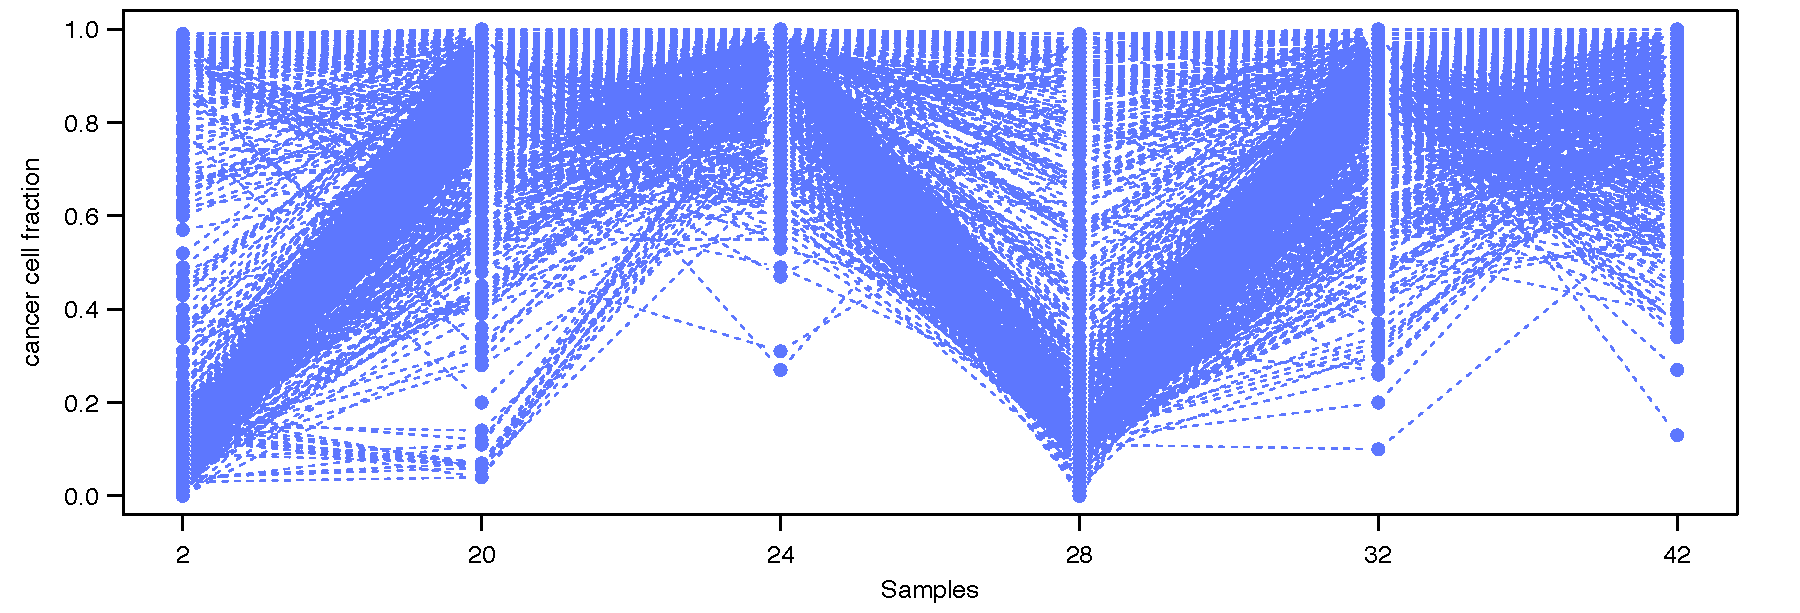
\includegraphics[width=.99\linewidth]{Figures/CASCADE/CA80/CA80.ccf_mutations.pdf}
	\caption[Cancer cell fractions of individual mutations for patient CA-J]{Cancer cell fractions of individual mutations of cluster 2 containing TP53 mutations for patient CA-J : each dot represented a distinct variant. Variants were connected with a dotted line to the same variant in other samples. Mutations were clustered with PhylogicNDT; } \label{fig:ca80ccfMuts}
\end{figure}


PhylogicNDT analysis revealed a high degree of subclonality, consistent with the results from PURPLE. However, the low tumour purity of samples 2 and 28 lead to unrealistic clustering of variants in these samples. While the TP53 mutation was not found in either sample 2 or sample 28 (\autoref{fig:ca80heatmap}), the cluster containing this mutation was assigned a 100\% cancer cell fraction overall. As the individual mutations do show multiple substructures in this cluster, for example connecting 2 and 20 at low ccf as well as high, and parameter tuning did not lead to a more granular representation, we considered the results to be low quality and not interpretable (\autoref{tab:ca80cnv}, \autoref{fig:ca80ccfMuts}).


%we clear all floats before we go to the next patient
\cleardoublepage

%%%%%%%%%%%%%%%%%%%%%%%%%%%%%%%%%%%%%%%%%%%%%%%%%%%%%%%%%%%%%%%%%%%%%%%%%%%%%%%%%%%%%%%
%                               Patient CA82                                          %
%%%%%%%%%%%%%%%%%%%%%%%%%%%%%%%%%%%%%%%%%%%%%%%%%%%%%%%%%%%%%%%%%%%%%%%%%%%%%%%%%%%%%%%


\subsection{Patient CA-K}
\label{cascade-sec:CA82}

This 69 year old was a male patient who presented with multifocal lung adenocarcinoma without distant metastasis. The most PET avid location (left upper lung) was designated the primary site over the two other less avid locations (right upper lung and left lower lung). Initial treatment with the tyrosine kinase inhibitor Gefitinib was stopped when the dominant lung lesion and a hilar node lesion showed signs of progression and he was changed to Afatinib. A CT scan after 50 months showed a mild increase at the primary site, stable disease in satellite nodules and no new metastatic sites. After short treatment with Erlotinib, molecular pathology of a biopsy revealed the acquired EGFR~T790M resistance mutation. Enrolment in the CLOVIS trial involving treatment with the EGFR tyrosine kinase inhibitor Rociletinib and chemotherapy was ceased due to disease progression. Biopsy 2 confirmed the T790M mutation and therapy with Osimertinib was started, which led to slowly progressive disease. Due to new intracranial disease, and increase in lung and renal disease treatment was switched to the PD-1 inhibitor Nivolumab, but no remission was achieved and the patient died after 103 months (\autoref{fig:ca82timeline}).



\begin{figure}[ht]
\centering
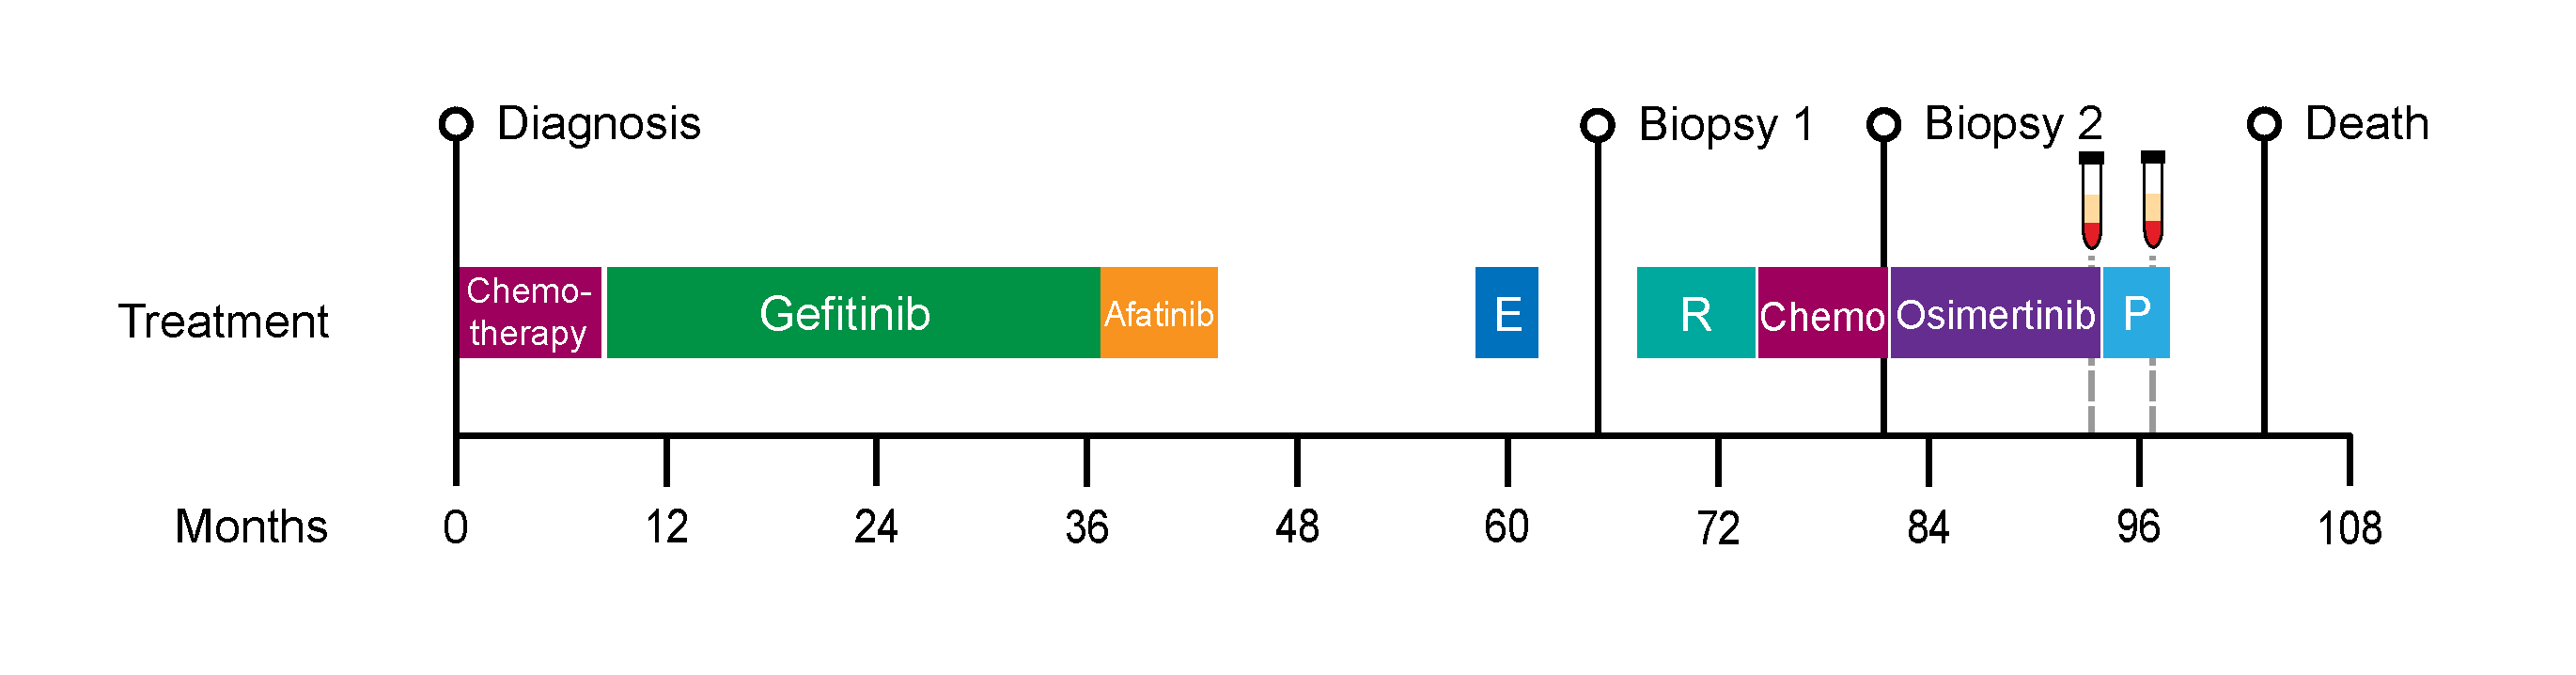
\includegraphics[width=.99\linewidth]{Figures/CASCADE/CA82/CA-K_timeline}
\caption[Timeline of patient CA-K from diagnosis until death]{Timeline of patient CA-K from diagnosis until death: Diagnostic biopsy detected EGFR~L858R positive lung adenocarcinoma;  Biopsy 1 after 66 months showed additional EGFR~T790M mutation; Biopsy 2 showed no additional variants; one blood sample was taken towards the end of Osimertinib treatment and one second one during PD-1 checkpoint blockade treatment. E: Erlotinib; R: Rociletinib; P: PD-1 inhibitor} \label{fig:ca82timeline}
\end{figure}

Analysis of the plasma sample collected five  months prior to the death of the patient with the AVENIO commercial kit revealed an \textit{AKT}, a \textit{KRAS}, and several \textit{EGFR} resistance mutations with high confidence at very low allele frequency. Out of the reported low confidence somatic variants, several more known \textit{EGFR} resistance alterations could be validated in the autopsy samples. Due to the overall low VAF of found variants, we assumed a low ctDNA fraction of the sample. Nevertheless,  the multiple \textit{EGFR} mutations suggested a high polyclonality of the disease and a purely genomically \textit{EGFR} driven cancer  (\autoref{tab:ca82plasma}). While these results suggest that a high degree of the final heterogeneity was already present, the longitudinal distance of the plasma sample to the autopsy samples suggests subsequent evolution, which could also be seen absence of the \textit{APC} mutation in the plasma (\autoref{fig:ca82heatmap}).

\begin{table}[ht]
\caption[Somatic variants found in plasma with AVENIO sequencing for patient CA-K]{Somatic variants found in plasma with AVENIO sequencing for patient CA-K: all high confidence variants are shown; low confidence variants also seen at autopsy in any sample were also selected}\label{tab:ca82plasma}
\centering
\rowcolors{2}{gray!15}{white}
\begin{tabular}{|c|c|c|c|c|}
\toprule
\hline
 \rowcolor{gray!50}
\textbf{Gene} & \textbf{Change} & \textbf{VAF (\%)} & \textbf{High confidence} & \textbf{Found at autopsy}\\
\hline
 AKT1 & Glu17Lys & 0.88 & \cellcolor{green!9} & \cellcolor{green!9}True\\
 KRAS & Gly12Val & 0.18 & \cellcolor{green!9} & \cellcolor{red!9}\\
 \cellcolor{white} & Asp761Tyr & 0.05 & \cellcolor{green!9} & \cellcolor{red!9}\multirow{-2}{*}{False} \\
 \cellcolor{white} & Thr790Met & 0.71 & \cellcolor{green!9} & \cellcolor{green!9}\\
 \cellcolor{white} & Cys797Ser & 0.26 & \cellcolor{green!9} & \cellcolor{green!9}\\
 \cellcolor{white} & Leu858Arg & 1.03 & \cellcolor{green!9}\multirow{-6}{*}{True} & \cellcolor{green!9}\\
 \cellcolor{white} & Leu718Gln & 0.69 & \cellcolor{red!9} & \cellcolor{green!9}\\
 \cellcolor{white} \multirow{-6}{*}{EGFR}& Ser720Thr & 0.67 & \cellcolor{red!9}\multirow{-2}{*}{False} & \cellcolor{green!9}\multirow{-5}{*}{True}\\
 
 \hline
\bottomrule
\end{tabular}
\end{table} 



At autopsy 18 sites were resected and biobanked and seven high quality representative samples from different organs were selected for WGS (\autoref{fig:ca82schematic}, \autoref{tab:ca82wgsSamples}) and analysed with the standard workflow (\autoref{cascade-sec:workflow}). 




\begin{figure}[ht]
\centering
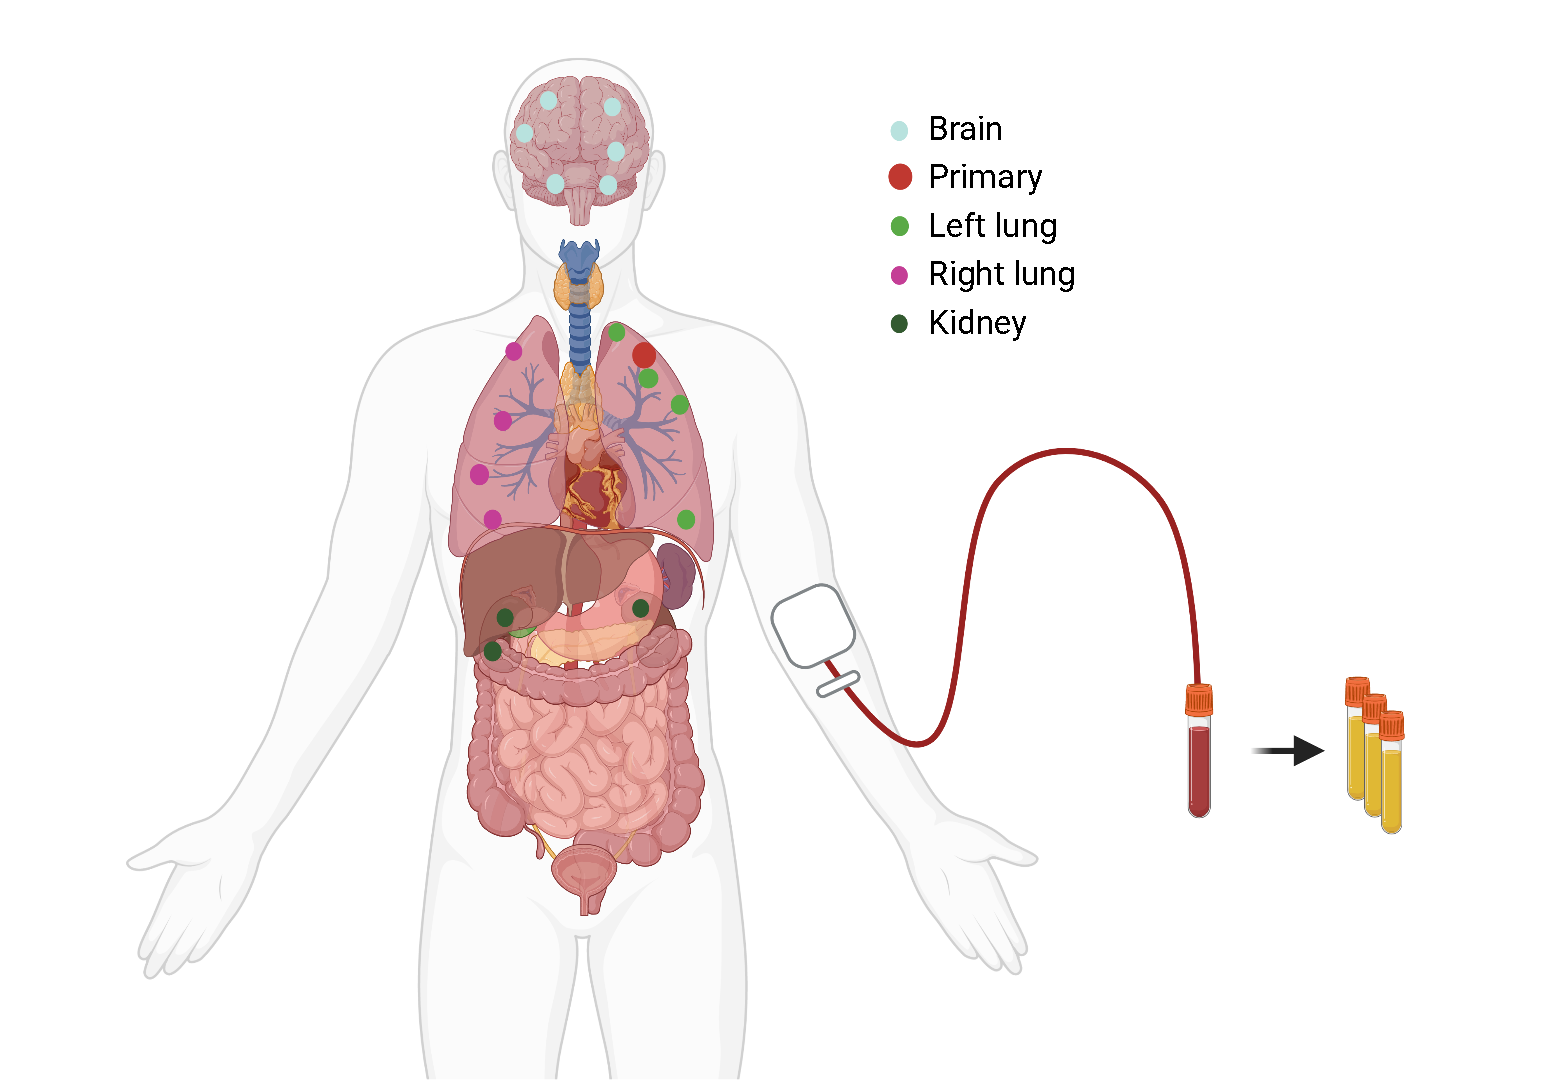
\includegraphics[width=.99\linewidth]{Figures/CASCADE/CA82/CA-K_schematic_CA82_organColours}
\caption[Schematic of analysed tumour lesions in patient CA-K]{Schematic of analysed tumour lesions in patient CA-K: Primary diagnostic sample shown in red; All 17 autopsy samples were coloured by organ they were collected from: Brain (6), left lung (4), right lung (4), kidney (3); Additionally to the post mortem blood sample, two serial blood samples were taken (\protect\autoref{fig:ca82timeline})} \label{fig:ca82schematic}
\end{figure}

\begin{table}[ht]
\caption[Autopsy samples sequenced for patient CA-K]{Autopsy samples sequenced for patient CA-K: Sample number is the internal sample collection during CASCADE autopsy, the organ of the sample, the fraction of tumour cells from H\& E stain and the pathology of the tumour sample. Dx: diagnostic sample}\label{tab:ca82wgsSamples}
\centering
\rowcolors{2}{gray!15}{white}
\begin{tabular}{|c|c|c|c|c|}
\toprule
\hline
 \rowcolor{gray!50}
\textbf{Sample number} & \textbf{Organ} & \textbf{H\&E} & \textbf{Type}\\
\hline
 Dx & left lung core & 0.8 & \cellcolor{white} \\
 1 & right kidney & 0.7 & \cellcolor{white} \\
 4 & right upper lung & 0.8 & \cellcolor{white} \\
 5 & right lower lung & 0.7 & \cellcolor{white} \\
 6 & right middle lung & 0.7 & \cellcolor{white} \\
 8 & left lower lung & 0.9 & \cellcolor{white} \\
 9 & left upper lung & 0.5 & \cellcolor{white} \\
 13 & left brain & 0.5 & \cellcolor{white}\multirow{-8}{*}{adenocarcinoma} \\
 \hline
\bottomrule
\end{tabular}
\end{table} 


Joint somatic variant calling on all autopsy samples revealed significant genetic heterogeneity of resistance mechanisms present at each site. While the initial EGFR~L858R mutation was still present in all sequenced lesions, the left lower lung sample (8) was the only one with a homozygous variant. All other samples presented with 50\% VAF for the activating mutation. Biopsy 1, 66 months after diagnosis, showed the additional EGFR~T790M mutation, but at autopsy sample 1 (adrenal gland) did not show evidence of the mutation at all and samples 8, 9, and 13 (left lung and brain) exhibited the variant at subclonal frequencies ($<30\%$ VAF). Either the mutation was already subclonal at biopsy, or the resistance was outcompeted by a different clone due to the Osimertinib treatment which targets T790M. The adrenal gland lesion, which did not contain the T790M mutation, instead presented with two other clonal EGFR mutations (S720T and L718Q) which are both known resistant mechanisms to Osimertinib \cite{Johnson2010,Bersanelli2016}.

Additionally the mutations AKT1~G17L and APC~E190Ter bifurcated the the autopsy samples into two groups, because the variants were mostly mutually exclusive, where only samples 8 and 9 showed both the stop gained \textit{APC} mutation at 100\% VAF with very low VAF of the \textit{AKT1} mutation. Furthermore, several \textit{EGFR} mutations also showed different spatial clonal abundance. Multiple samples exhibited different C797 substitutions both of which are known resistance mechanisms to Osimertinib \cite{Wang2016,Leonetti2019}: Sample 4 contained the EGFR~C797G mutation at 7\% VAF whereas samples 6, 8, and 9 had a C797S mutation at 1\%, 14\%, and 22\% VAF respectively. However, while 8 shared the sample protein change (C797S) the genomic change was different to both sample 6 and 9. Only sample 4 contained EGFR~L792H as a subclonal mutation at 11\% VAF and both sample 1 and 6 contained a subclonal EGFR~S720T mutation, another known resistance mechanisms \cite{Johnson2010,Zhang2018b}. Additionally to the adrenal sample both lower and middle lower lung samples contained EGFR~L718Q. 
Lastly, all but sample 8 contain the \textit{SMAD4} frameshift mutation at a median cancer cell fraction of 73\% (min: 16\%, max: 100\%) (\autoref{fig:ca82heatmap}).

These genomic changes grouped the samples according to their anatomical location, with right kidney (1) and left brain (13) as outliers, but left (8 and 9) and right lung (4, 5, and 6) samples clustering together (\autoref{fig:ca82phylo}).

\begin{figure}[ht]
	\centering
	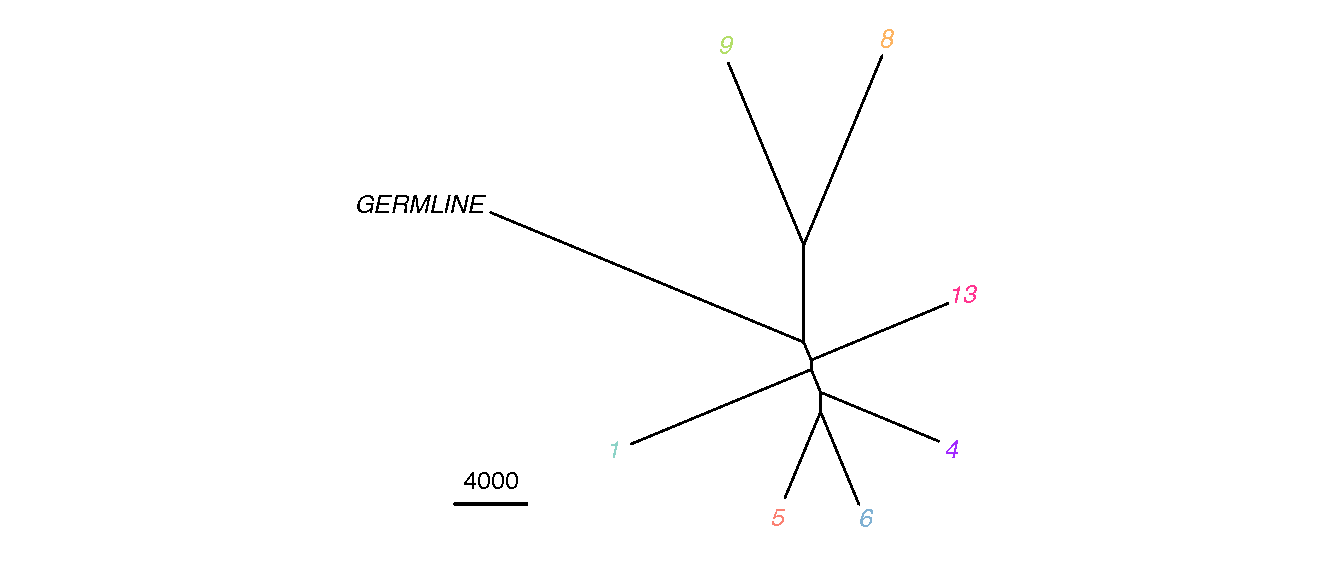
\includegraphics[width=.99\linewidth]{Figures/CASCADE/CA82/CA82phylo.pdf}
	\caption[Phylogeny of autopsy samples from patient CA-K]{Phylogeny of autopsy samples from patient CA-K; reconstructed with all somatic SNVs and InDels. Ruler symbolises 4000 variants difference} \label{fig:ca82phylo}
\end{figure}


\begin{figure}[htp]
\centering
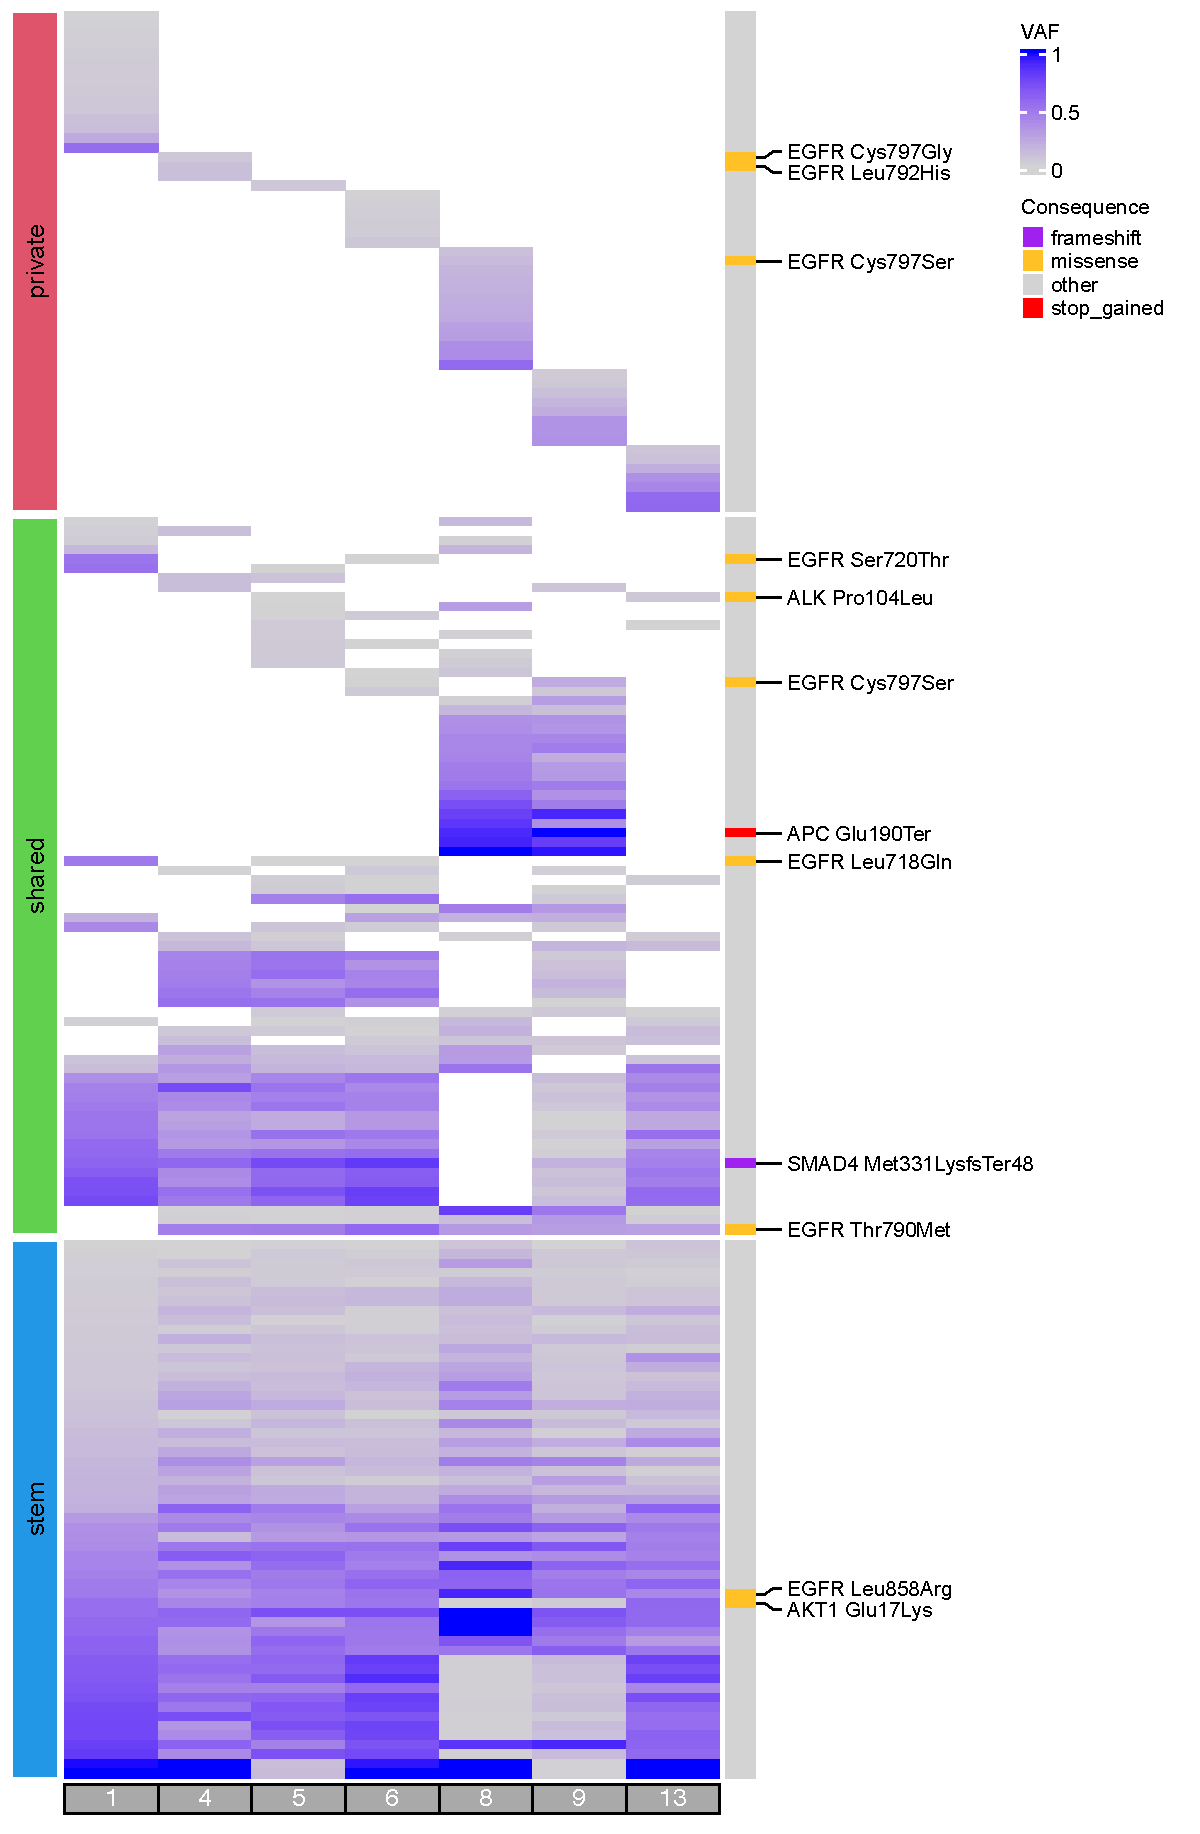
\includegraphics[width=.99\linewidth]{Figures/CASCADE/CA82/CA82varHeatmap.pdf}
\caption[Heatmap of driver gene variants in patient CA-K]{Heatmap of driver gene variants in patient CA-K: Protein altering mutations are highlighted with their HGVSp notation; non protein altering mutations are grouped as ``other``.} \label{fig:ca82heatmap}
\end{figure}


Similar to the short variants, structural variants and copy number changes also showed a difference between samples 8 and 9 compared to the rest. While all samples showed inversions on chromosome 6, 8 and 9 with fusions between chromosome 1 and 18, chromosome 6 and 8 and chromosome 8 and 9, samples 8 and 9 also showed a fusion of chromosome 3 with 18 and additional inversions on chromosome 18. The additional inversions and haploinsufficiency directly affect \textit{SMAD4}. These structural changes complemented the ``missing`` \textit{SMAD4} frameshift mutation in these samples and suggested a key role of \textit{SMAD4} in the resistance to treatment.

Samples 8 and 9 were the only samples in the patient with significantly amplified copy numbers resulting in a whole genome duplication, however they still exhibited the same pattern of loss of heterozygosity. In all samples we observed a copy number gain in the q arm of chromosome 1 amplifying both \textit{NTKR1} and \textit{DDR2} with a loss of heterozygosity for \textit{NRAS} and \textit{MTOR} on the p arm of the same chromosome. The loss of heterozygosity presented in all samples on chromosome 3 reduced the representation of \textit{TM4SF1}, \textit{PIK3CA}, and \textit{USP13}, however in both sample 8 and 9 the other chromosome was amplified leading to a copy number neutral area. The loss of heterozygosity on chromosome 5 leads to a haploinsufficiency for \textit{APC}, \textit{PIK3R1}, \textit{CSF1R}, \textit{PDGFRB}, and \textit{FLT4} for all samples, which combined with the stop mutation in samples 8 and 9 is suggestive of a common resistance pathway. The loss of heterozygosity on chromosome 8 affected \textit{TUSC3} and \textit{FGFR1}. No lung cancer driver genes were affected by the loss of heterozygosity on chromosome 15. The seemingly heterozygous loss of chromosome X resulted in the loss of \textit{ARAF} and \textit{AR} as a consequence, but the loss must have been subclonal given the sex of the patient was male. Lastly, the additional copy number loss only present in both samples 8 and 9 affected \textit{JAK2}, \textit{CD274}, and \textit{PDCD1LG2} and these samples also showed \textit{EGFR} amplification in contrast to all other samples (\Autoref{fig:ca82.1circos,fig:ca82.4circos,fig:ca82.5circos,fig:ca82.6circos,fig:ca82.8circos,fig:ca82.9circos,fig:ca82.13circos},  \autoref{tab:ca82cnv}). 


\begin{figure}[htp]
\centering
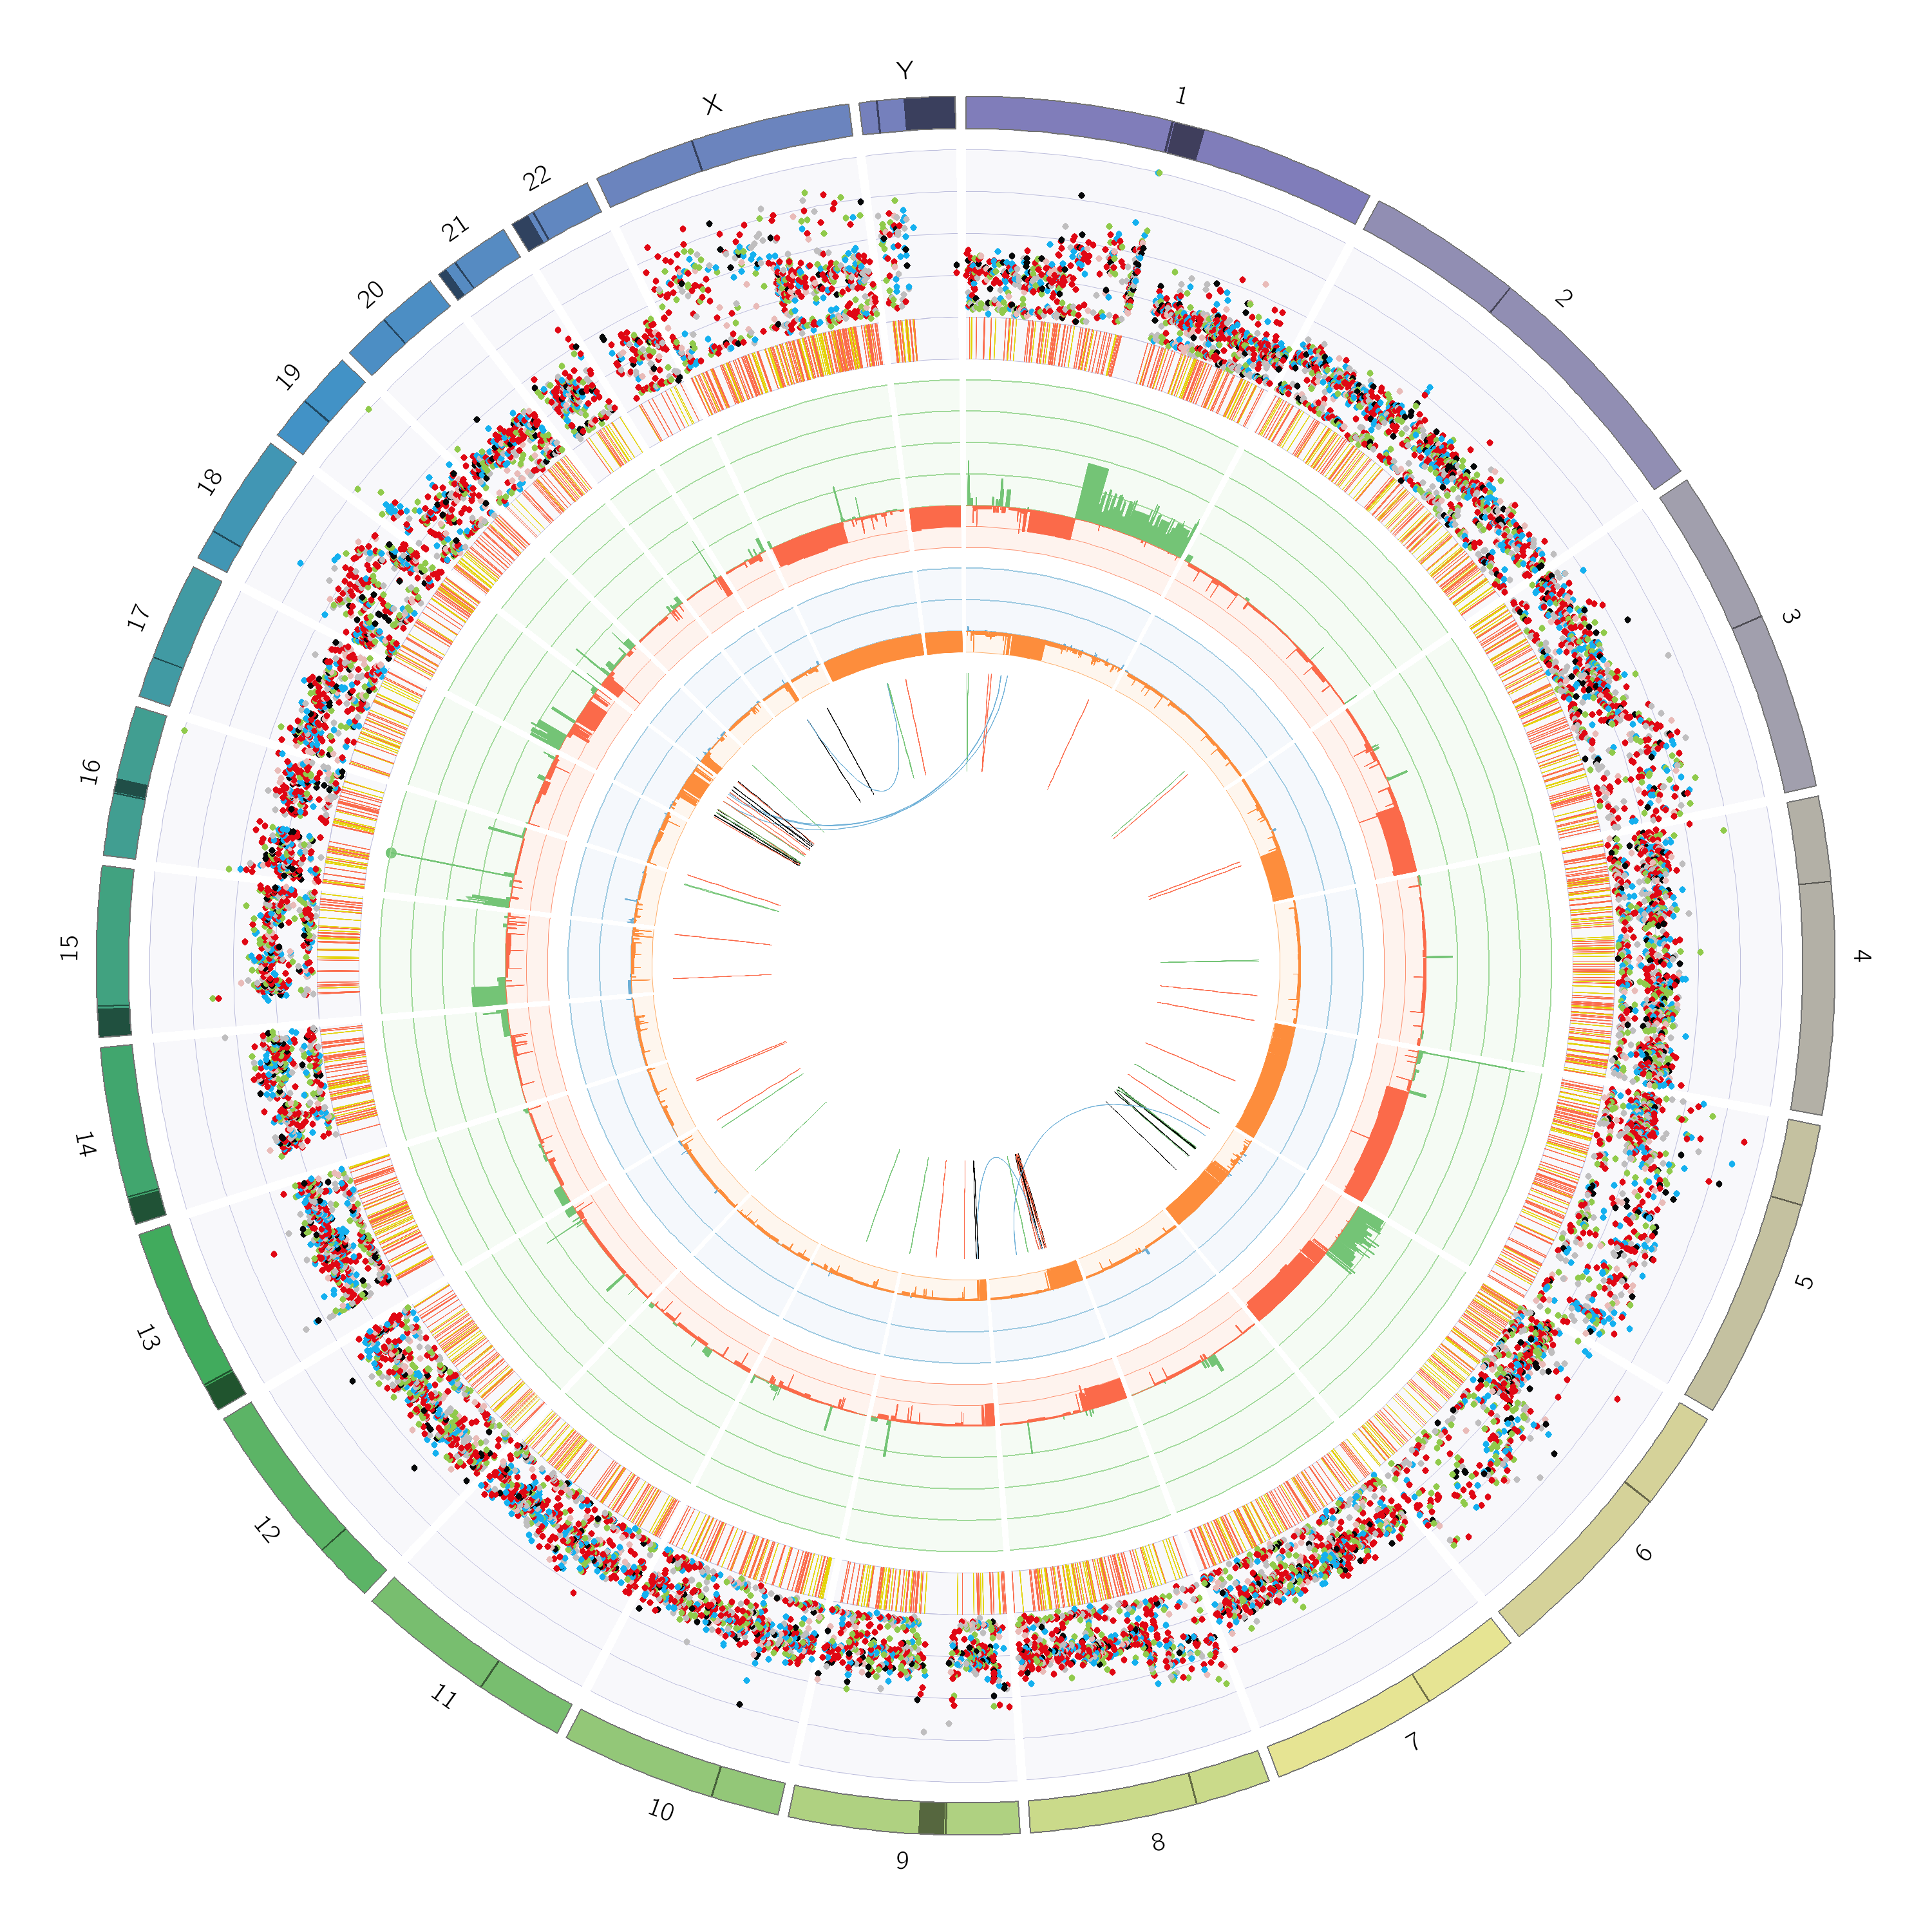
\includegraphics[width=.99\linewidth]{Figures/CASCADE/CA82/CA82-1.circos.png}
\caption[Circos plot of patient CA-K sample 1]{Circos plot of patient CA-K sample 1: outer first ring shows the canonical chromosomes with gaps (centromere, heterochromatin,...) highlighted as darker areas; second ring visualises all somatic SNVs corrected for tumour purity and scaled from 0 to 1, the colour representing the base change of SNV like in \protect\textcite{Alexandrov2013}; vertical lines directly under the SNVs symbolise InDels, with yellow for insertions and red for deletions; the third ring shows the total copy number alterations, with green showing a copy number gain and red a loss, dots at the outer border show a copy number greater than four; the last ring shows the minor copy number, with blue depicting a gain and orange a loss, this ring allows the detection of copy number neutral changes, like loss of heterozygosity; the center shows all structural variants: translocations in blue, deletions in red, insertions in yellow, tandem duplications in green and inversions in black.} \label{fig:ca82.1circos}
\end{figure}



\begin{figure}[htp]
\centering
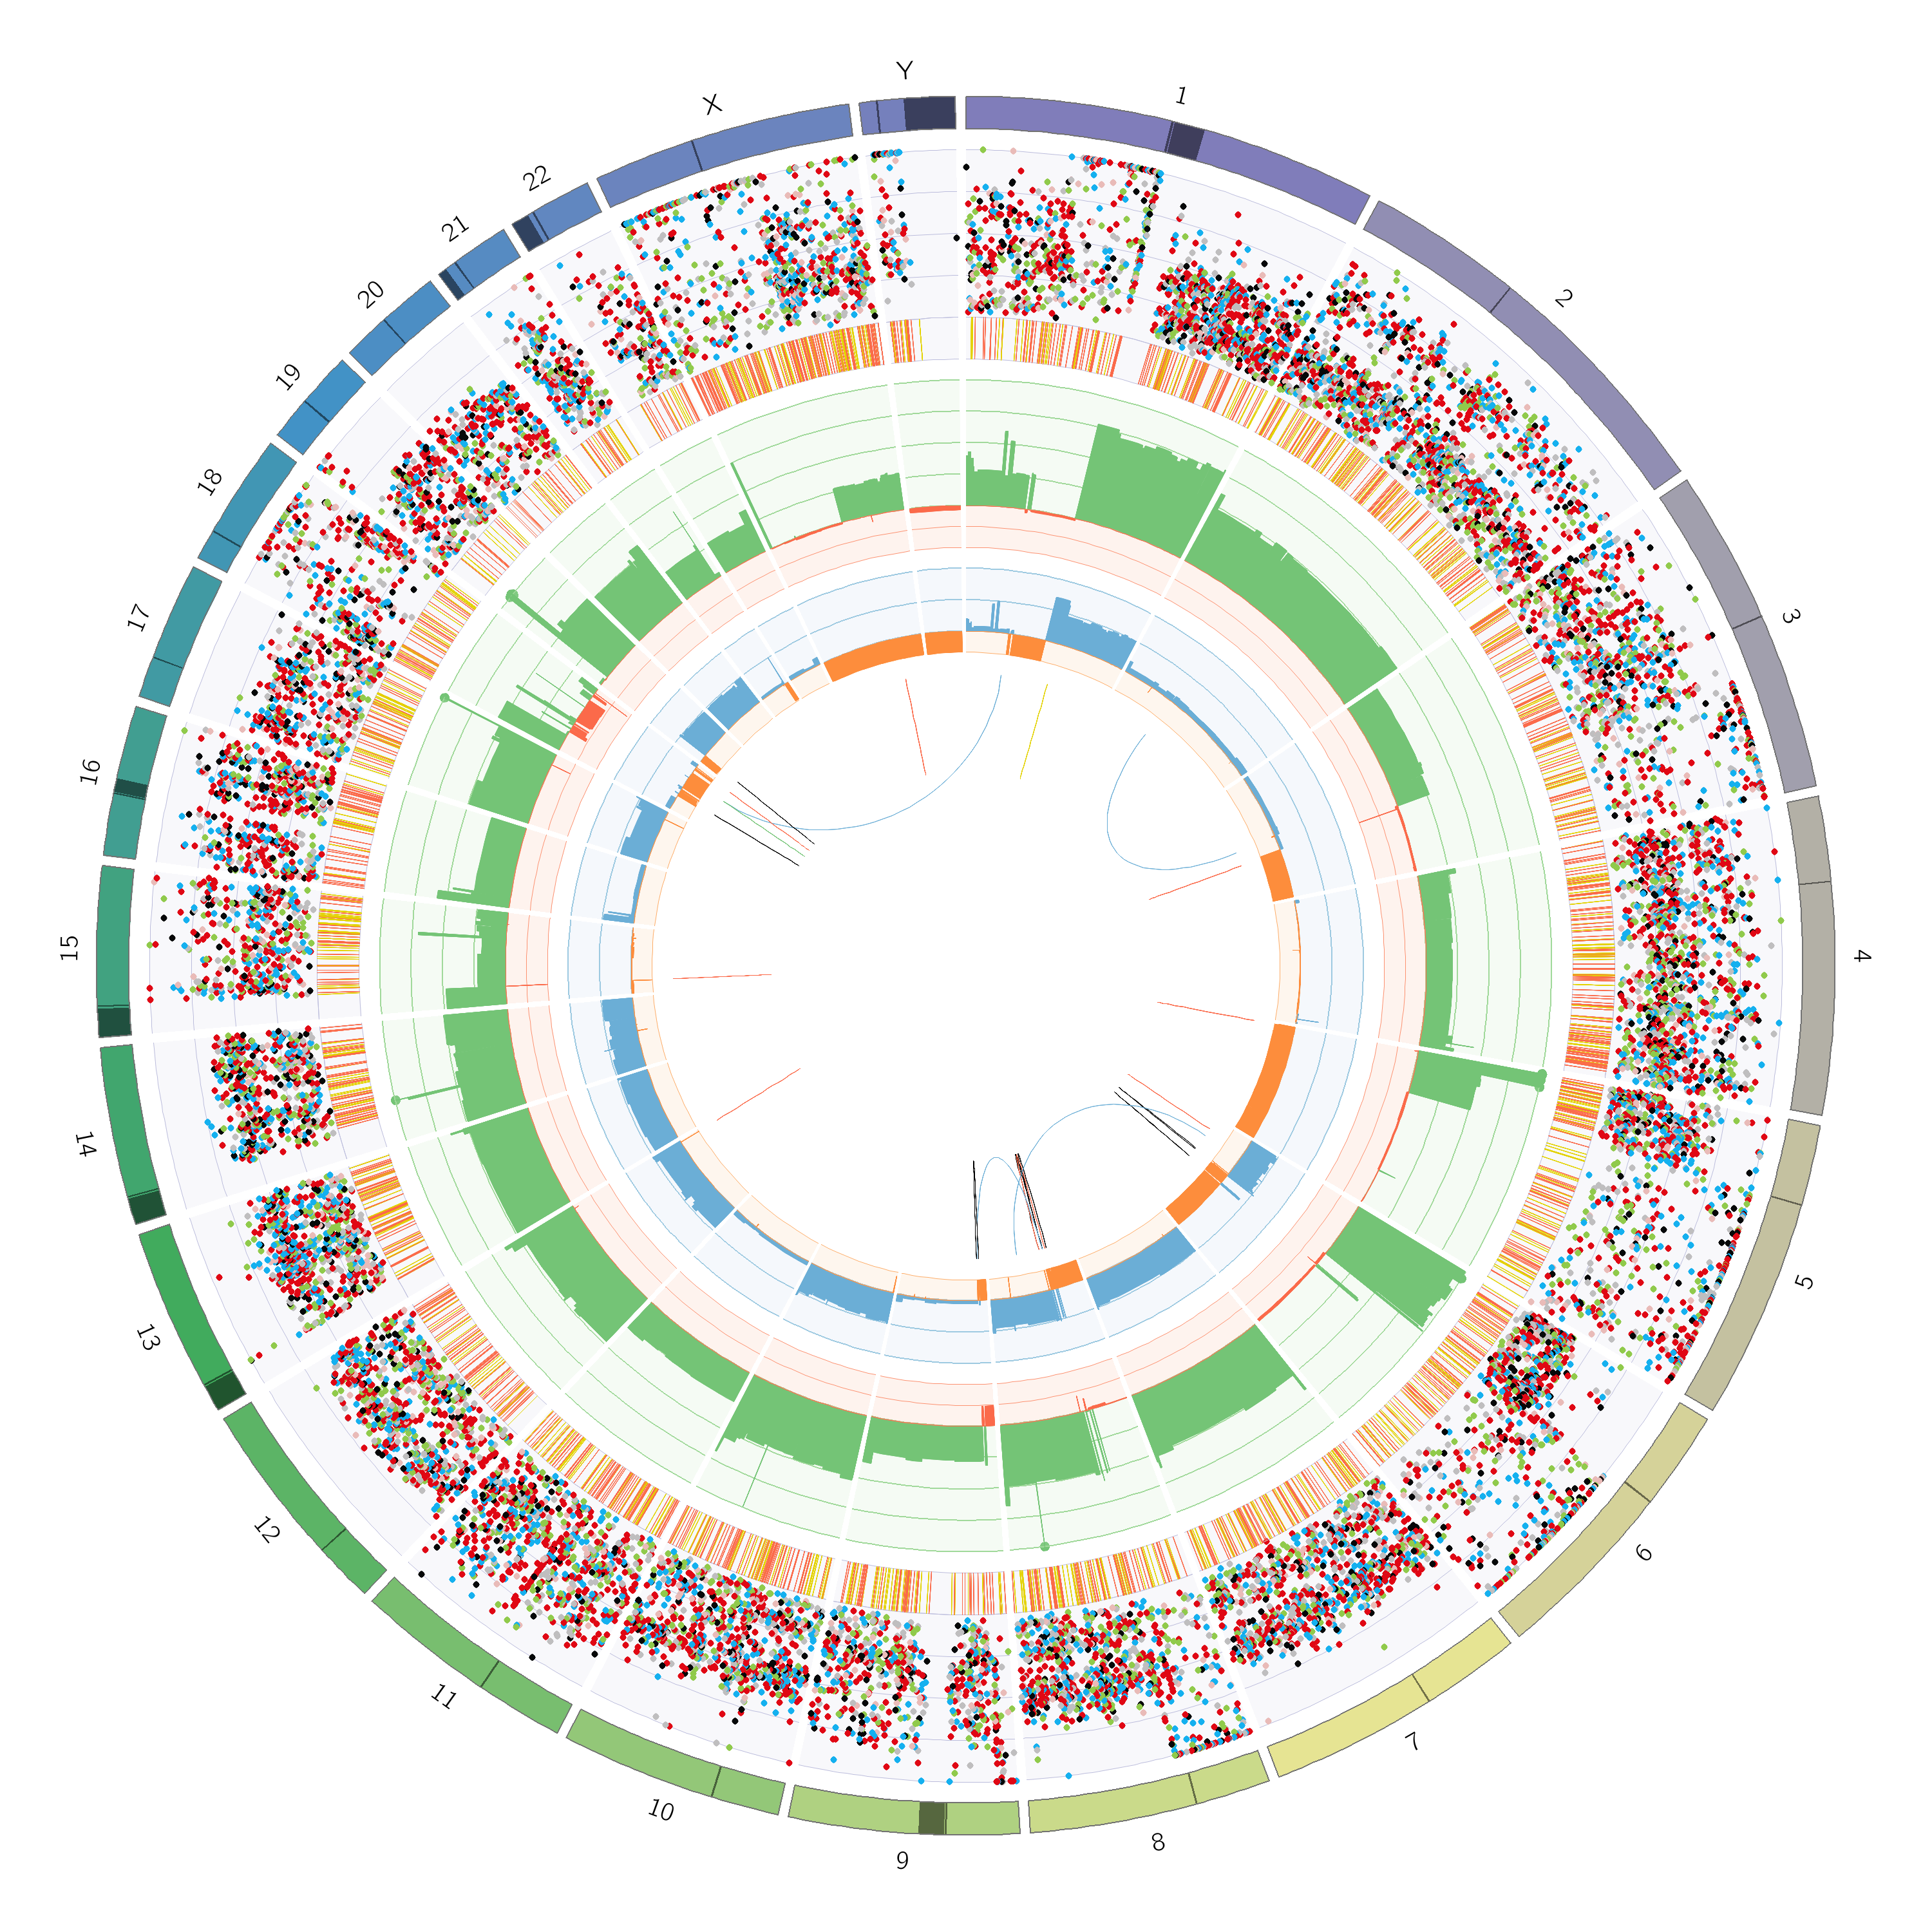
\includegraphics[width=.99\linewidth]{Figures/CASCADE/CA82/CA82-8.circos.png}
\caption[Circos plot of patient CA-K sample 8]{Circos plot of patient CA-K sample 8: outer first ring shows the canonical chromosomes with gaps (centromere, heterochromatin,...) highlighted as darker areas; second ring visualises all somatic SNVs corrected for tumour purity and scaled from 0 to 1, the colour representing the base change of SNV like in \protect\textcite{Alexandrov2013}; vertical lines directly under the SNVs symbolise InDels, with yellow for insertions and red for deletions; the third ring shows the total copy number alterations, with green showing a copy number gain and red a loss, dots at the outer border show a copy number greater than four; the last ring shows the minor copy number, with blue depicting a gain and orange a loss, this ring allows the detection of copy number neutral changes, like loss of heterozygosity; the center shows all structural variants: translocations in blue, deletions in red, insertions in yellow, tandem duplications in green and inversions in black.} \label{fig:ca82.8circos}
\end{figure}


\begin{table}[ht]
\caption[Copy number analysis results for patient CA-K]{Copy number analysis results for patient CA-K: results are taken from the best fit result of PURPLE; WG: whole genome}\label{tab:ca82cnv}
\centering
\rowcolors{2}{gray!15}{white}
\begin{tabular}{|c|c|c|c|c|}
\toprule
\hline
 \rowcolor{gray!50}
\textbf{Sample number} & \textbf{purity} & \textbf{ploidy} & \textbf{polyclonal \%} & \textbf{WG duplication}\\
\hline
 1 & \num{0.78} &	 \num{1.84} &	\num{7.62} & False	\\
 4 & \num{0.48} & \num{1.84} & \num{4.80} & False \\
 5 & \num{0.58} & \num{1.88} & \num{1.02} & False \\
 6 & \num{0.79} & \num{1.86} & \num{6.93} & False \\
 8 & \num{0.30} & \num{3.40} & \num{6.44} & True \\
 9 & \num{0.69} & \num{3.45} & \num{8.32} & True \\
 13 & \num{0.47} & \num{1.90} & \num{0.05} & False \\
 \hline
\bottomrule
\end{tabular}
\end{table} 

\begin{figure}[ht]
\centering	
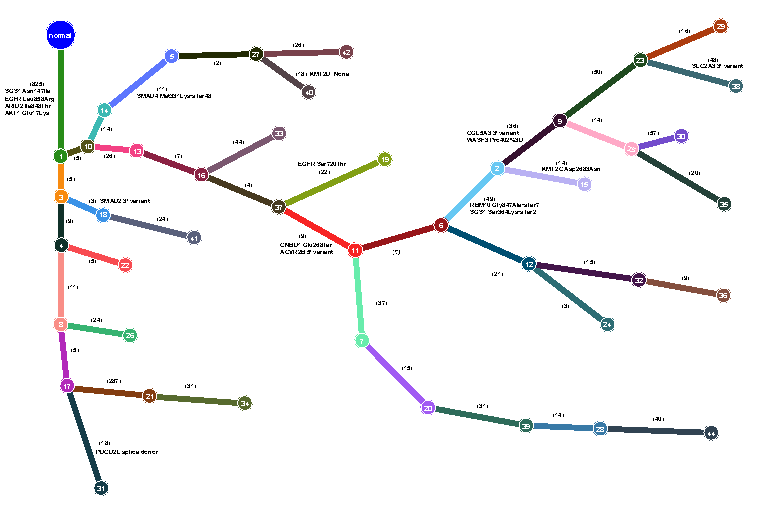
\includegraphics[width=.99\linewidth]{Figures/CASCADE/CA82/CA82.clonaltree.pdf}
\caption[Clonal evolutionary tree CA-K]{Clonal evolutionary tree of patient CA-K; Highest support tree for clustered ccf clones generated with PhylogicNDT; Support for clone is shown in parenthesis; Major driver alterations of clones were annotated; Clusters with less than 10 supporting variants were discarded} \label{fig:ca82.clonalTree}

\vspace{\floatsep}

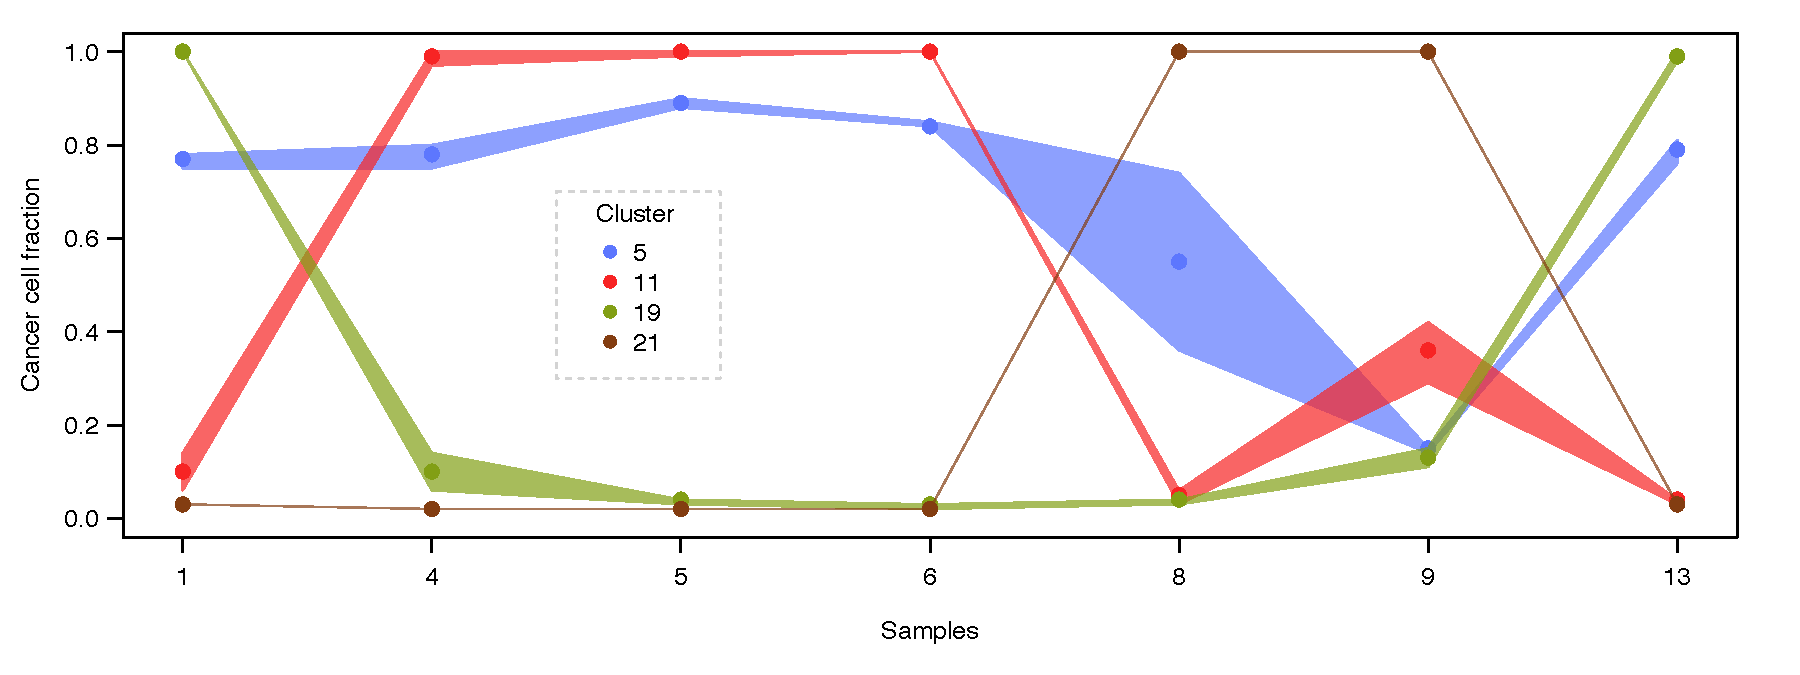
\includegraphics[width=.99\linewidth]{Figures/CASCADE/CA82/CA82.ccf_cluster.pdf}
\caption[Cancer cell fraction of mutation clusters of clonal tree for patient CA-K]{Cancer cell fraction of mutation clusters of clonal tree for patient CA-K; transparent polygons show the 95\% confidence intervals. Clusters and cluster colours are taken from \protect\autoref{fig:ca82.clonalTree}} \label{fig:ca82.ccfCluster}

\end{figure}


Similar to the phylogeny, the clonal deconvolution with PhylogicNDT revealed a higher complexity of disease after a bottle neck, where the right side lung samples (samples 4, 5, and 6) all presented with a very high prevalence of cluster 11 and followed by clonal diversification after the CNBD1 stop-gained mutation. In contrast samples 1 and 13 (kidney and brain) showed an additional EGFR~S720W mutation separating the distant sites from the original lung disease. Finally, the original site of disease in the left lung lobe displayed less diversification, however the early split of cluster 1 into 10 and 3 splitting left lung and all other sites suggests early metastatic seeding (\Autoref{fig:ca82.clonalTree,fig:ca82.ccfCluster}). 



%we clear all floats before we go to the next patient
\cleardoublepage

%%%%%%%%%%%%%%%%%%%%%%%%%%%%%%%%%%%%%%%%%%%%%%%%%%%%%%%%%%%%%%%%%%%%%%%%%%%%%%%%%%%%%%%
%                               Patient CA86                                          %
%%%%%%%%%%%%%%%%%%%%%%%%%%%%%%%%%%%%%%%%%%%%%%%%%%%%%%%%%%%%%%%%%%%%%%%%%%%%%%%%%%%%%%%

\subsection{Patient CA-L}
\label{cascade-sec:CA86}

This 68 year old female ex-smoker presented with \textit{EGFR} mutant NSCLC, however after 12 months of the treatment with the EGFR inhibitor Erlotinib a transformation to small cell lung cancer (SCLC) was detected. While previously it was thought that the different subsets of lung cancers are distinct, more and more evidence is found showing neuroendocrine transformation as a resistance mechanism to targeted therapies not only in lung but also in prostate cancers \cite{Oser2015,Aggarwal2018}. The treatment was altered to chemotherapy and then PD-1 inhibition, however due to the loss of MHC-I antigen presentation of small cell lung cancer, the tumour failed to respond \cite{Burr2019} and the patient died after 29 months (\autoref{fig:ca86timeline}).

\begin{figure}[ht]
\centering
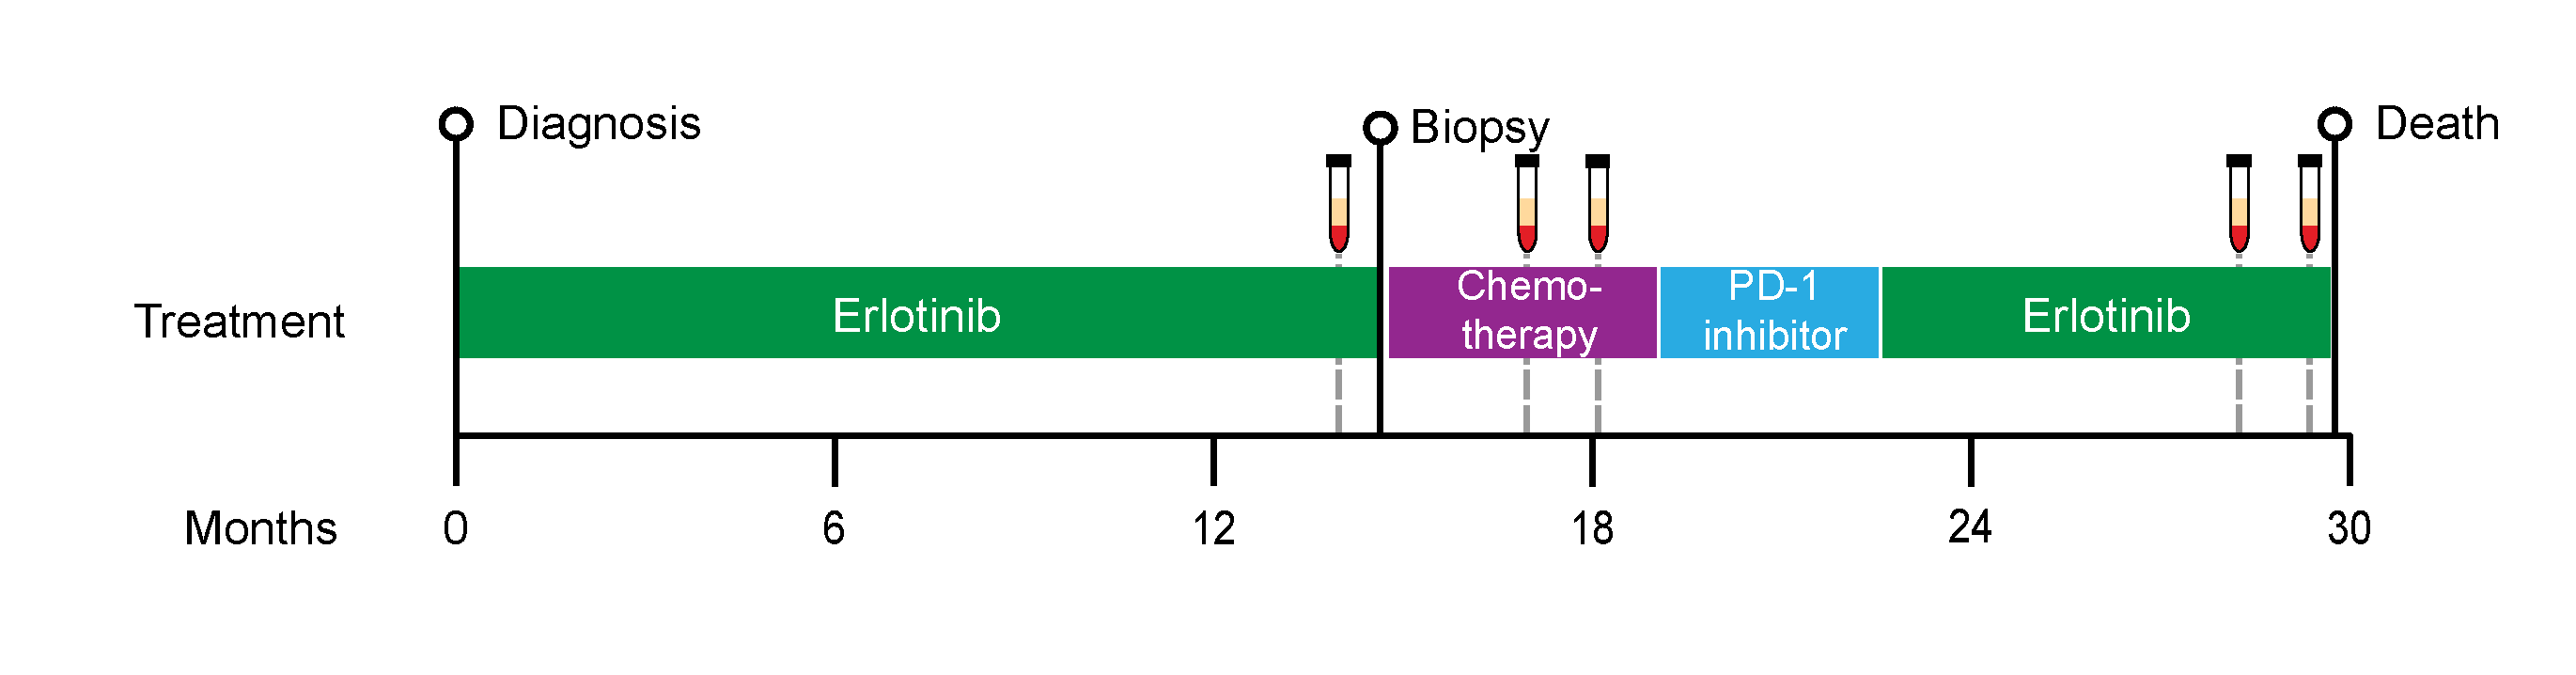
\includegraphics[width=.99\linewidth]{Figures/CASCADE/CA86/CA-L_timeline}
\caption[Timeline of patient CA-L from diagnosis until death]{Timeline of patient CA-L from diagnosis until death: Diagnostic biopsy detected EGFR exon 19 deletion positive lung adenocarcinoma;  Biopsy after 15 months Erlotinib treatment showed signs of small cell transformation; blood samples were taken at the end of the first Erlotinib treatment, during the chemotherapy treatment and 28 and 29 months after the initial diagnosis.} \label{fig:ca86timeline}
\end{figure}

During autopsy 25 lesions were resected and biobanked and representative samples, both adeno- and small cell carcinoma according to histology, were selected for WES (\autoref{fig:ca86schematic}, \autoref{tab:ca86wesSamples}) and analysed with the standard workflow (\autoref{cascade-sec:workflow}). For granular analysis of the transition from adeno- to small cell carcinoma, the progression sample after 15 months (P) was dissected to the individual types based on histology staining.


\begin{figure}[htp]
\centering
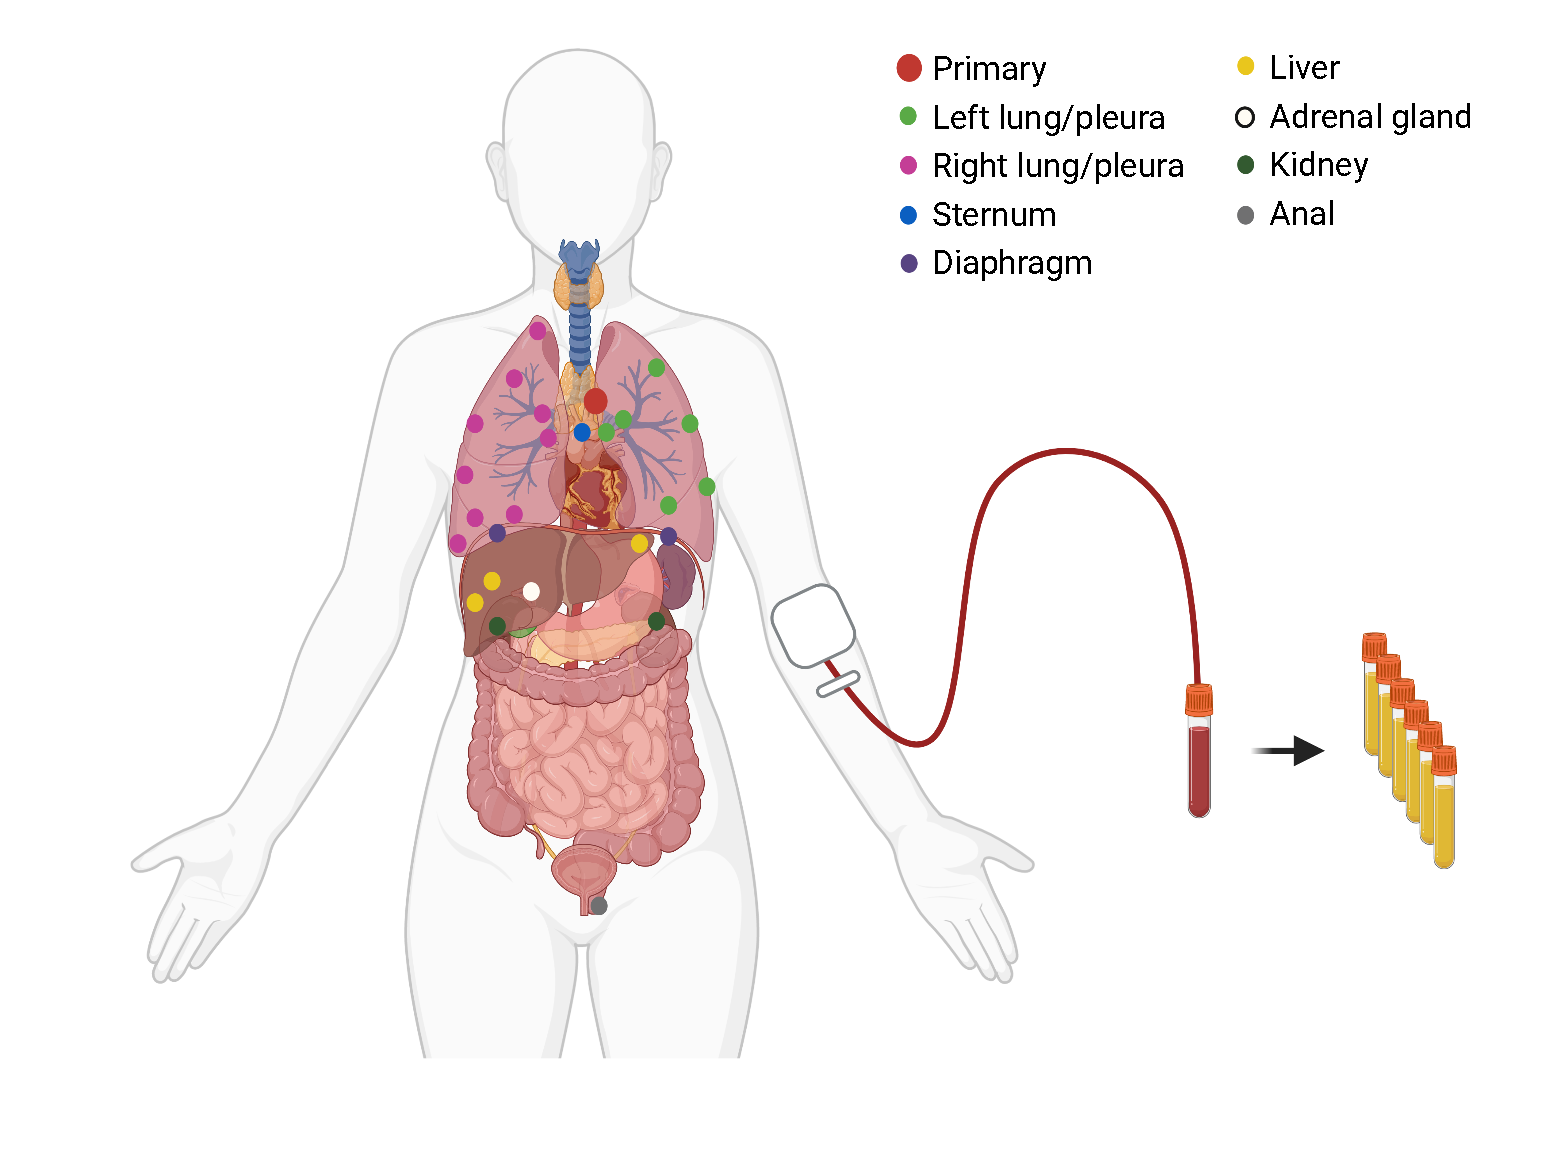
\includegraphics[width=.99\linewidth]{Figures/CASCADE/CA86/CA-L_schematic_CA86_organColours}
\caption[Schematic of analysed tumour lesions in patient CA-L]{Schematic of analysed tumour lesions in patient CA-L: Primary diagnostic sample shown in red; Samples are coloured by organ they were collected from: left lung (6), right lung (9), sternum (1), diaphragm (2), liver (3), adrenal gland (1) kidney (2), anal (1); Additionally to the post mortem blood sample, five serial blood samples were taken (\protect\autoref{fig:ca86timeline})} \label{fig:ca86schematic}
\end{figure}

\begin{table}[ht]
\caption[Autopsy samples sequenced for patient CA-L]{Autopsy samples sequenced for patient CA-L: Sample number is the internal sample collection during CASCADE autopsy, the organ of the sample, the fraction of tumour cells from H\& E stain and the pathology of the tumour sample. P.1/2: micro-dissected progression biopsy (80\% small cell, 20\% adeno)}\label{tab:ca86wesSamples}
\centering
\rowcolors{2}{gray!15}{white}
\begin{tabular}{|c|c|c|c|c|}
\toprule
\hline
 \rowcolor{gray!50}
\textbf{Sample number} & \textbf{Organ} & \textbf{H\&E} & \textbf{Type}\\
\hline
 P.1 & right lung core & \cellcolor{gray!15} & small cell \\
 P.2 & right lung core & \cellcolor{gray!15}\multirow{-2}{*}{>0.9} & adenocarcinoma \\
 8 & right upper lung & 0.9 & small cell \\
 17A & left lower lung & - & poorly differentiated adeno \\
 26 & right kidney & 1 & adenocarcinoma \\
 \hline
\bottomrule
\end{tabular}
\end{table} 

Even though not all samples had changed from adeno- to small cell carcinoma, all samples showed the \textit{TP53} ``stop gained`` mutation at 100\% VAF, showing that the  \textit{TP53} mutation was not sufficient for the histological transformation \cite{Offin2019}. Unsurprisingly, the samples that remained adeno (17A and 26) show a higher dependency on \textit{EGFR} which led to higher clonal abundance of the initial \textit{EGFR} exon 19 deletion and a subsequently higher VAF of EGFR~T790M, while the small cell transformed lung sample (8) acquired a secondary TP53~M40I mutation. No additional variants were close to clonal representation (\autoref{fig:ca86heatmap}).

Surprisingly even though the samples were taken at different times (one at progression and one at autopsy) the small cell transformed samples P.1 and 8 were evolutionarily more closely related and shared more variants, than to the sample P.2 which was taken at the same time. In contrast, the two adenocarcinoma samples taken at autopsy were clustered together. Additionally, the split of sites of small cell transformation and adenocarcinoma  already had happened before the progression sample and the small cell transformed samples appeared to be evolutionary different from samples 17A and 26. In general, the phylogeny suggested the presence of at least 3 distinct trajectories: one giving rise to the adeno sample at progression (P.2), one resulting in the small cell sample P.1 and its longitudinal successor sample 8 and lastly the two adenocarcinoma samples 17A and 26 (\autoref{fig:ca86phylo}).

\begin{figure}[ht]
	\centering
	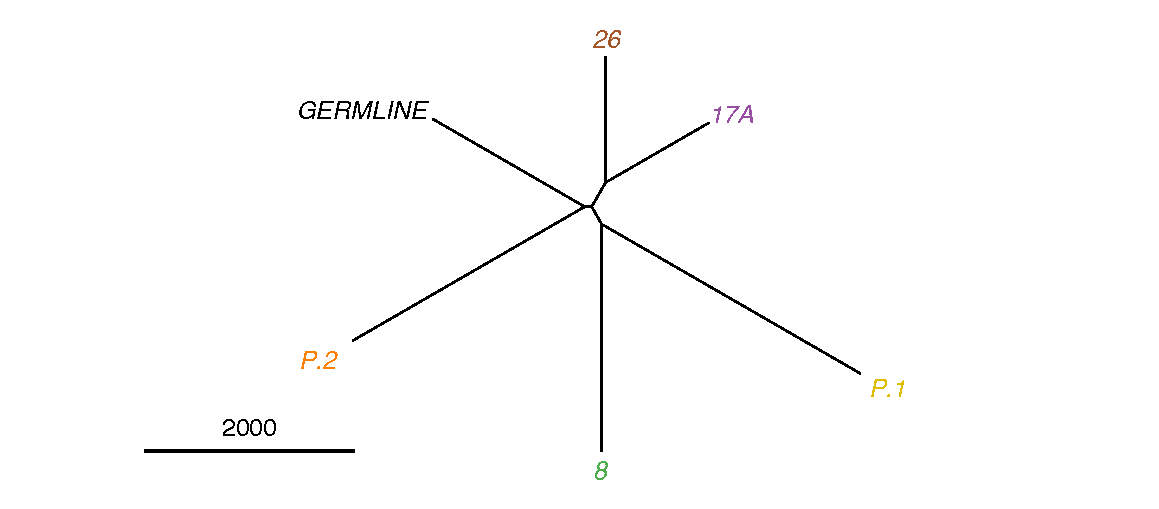
\includegraphics[width=.99\linewidth]{Figures/CASCADE/CA86/CA86phylo.pdf}
	\caption[Phylogeny of autopsy samples from patient CA-L]{Phylogeny of samples from patient CA-L; reconstructed with all somatic SNVs and InDels. Ruler symbolises 2000 variants difference.} \label{fig:ca86phylo}
\end{figure}


\begin{figure}[htp]
\centering
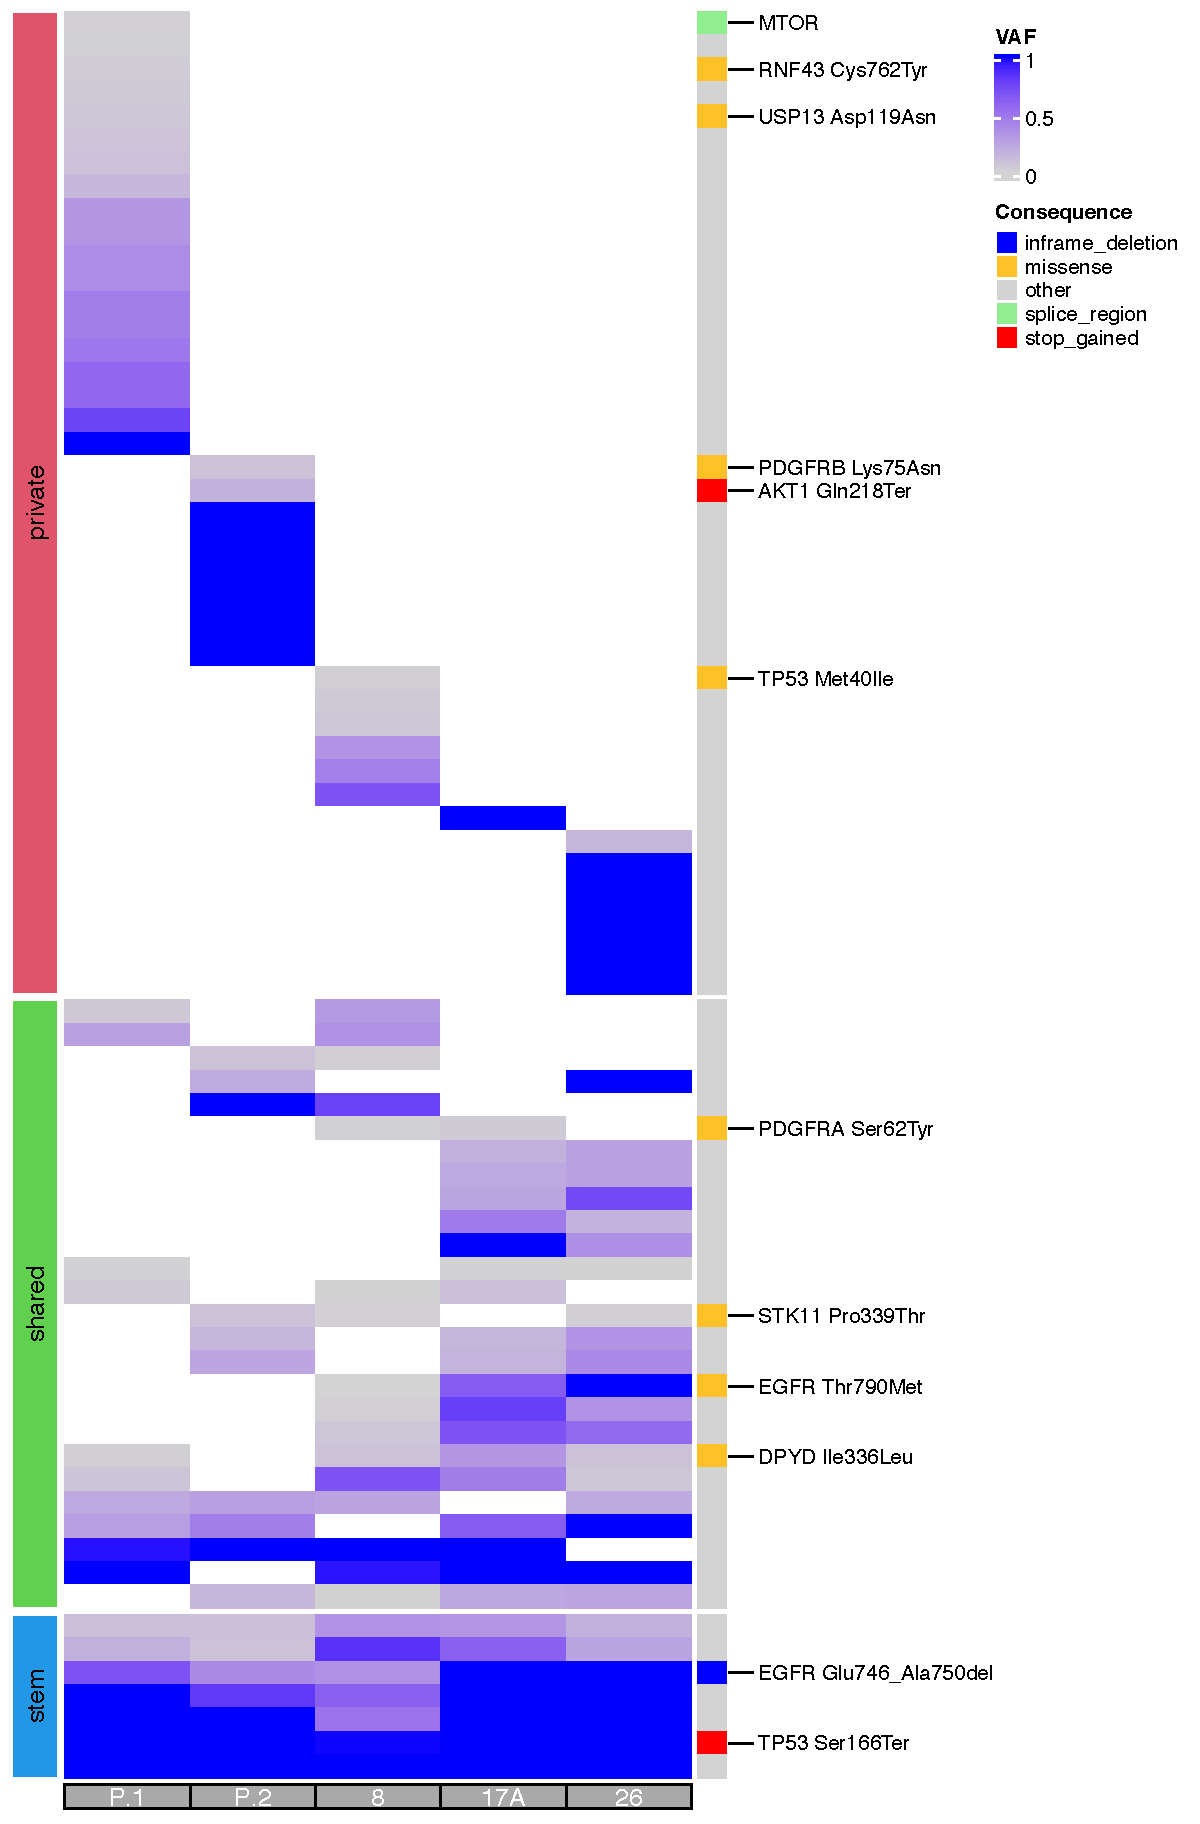
\includegraphics[width=.99\linewidth]{Figures/CASCADE/CA86/CA86varHeatmap.pdf}
\caption[Heatmap of driver gene variants in patient CA-L]{Heatmap of driver gene variants in patient CA-L: Protein altering mutations are highlighted with their HGVSp notation; non protein altering mutations are grouped as ``other``.} \label{fig:ca86heatmap}
\end{figure}


Copy number analysis with sequenza revealed a high prevalence of loss of heterozygosity in all samples,but both sample P.2 and 8 showed almost no copy number gains on chromosome 9 and 10 with sample 8 even extending through to chromosome 12. In general small cell transformed samples showed a higher level of copy number gain than the original adenocarcinoma. The difference in copy number in the two spatially intertwined types of cancers can only be attributed to the small cell transformation. Additionally to the increased overall ploidy of the small cell sample P.1 over P.2 (\autoref{tab:ca86cnv}), P.2 also lost chromosome X completely  (\autoref{fig:ca86.p1circos} vs. \autoref{fig:ca86.p2circos}). Interestingly, the small cell samples still had the same high amplification level of EGFR seen in the adenocarcinoma samples (min: 6 max: 13) suggesting the transformation retained EGFR based signalling. While commonly small cell transformation is associated with RB1 loss, the locus was amplified in all samples with a loss of heterozygosity. As this patient's sequencing was restricted to exonic regions, we could not rule out a regulatory defect. Interestingly, while the small cell transformed part of the progression sample (P.1) showed a heterozygous loss of chromosome X, the adenocarcinoma part (P.1) showed an almost complete loss of chromosome X, which could not be observed in any of the autopsy samples, which instead showed and amplification. This indicated, that the small cell transformation happened at multiple sites instead of being spread after the transformation (\Autoref{fig:ca86.p1circos,fig:ca86.p2circos,fig:ca86.8circos,fig:ca86.17Acircos,fig:ca86.26circos}), .

\begin{figure}[htp]
\centering
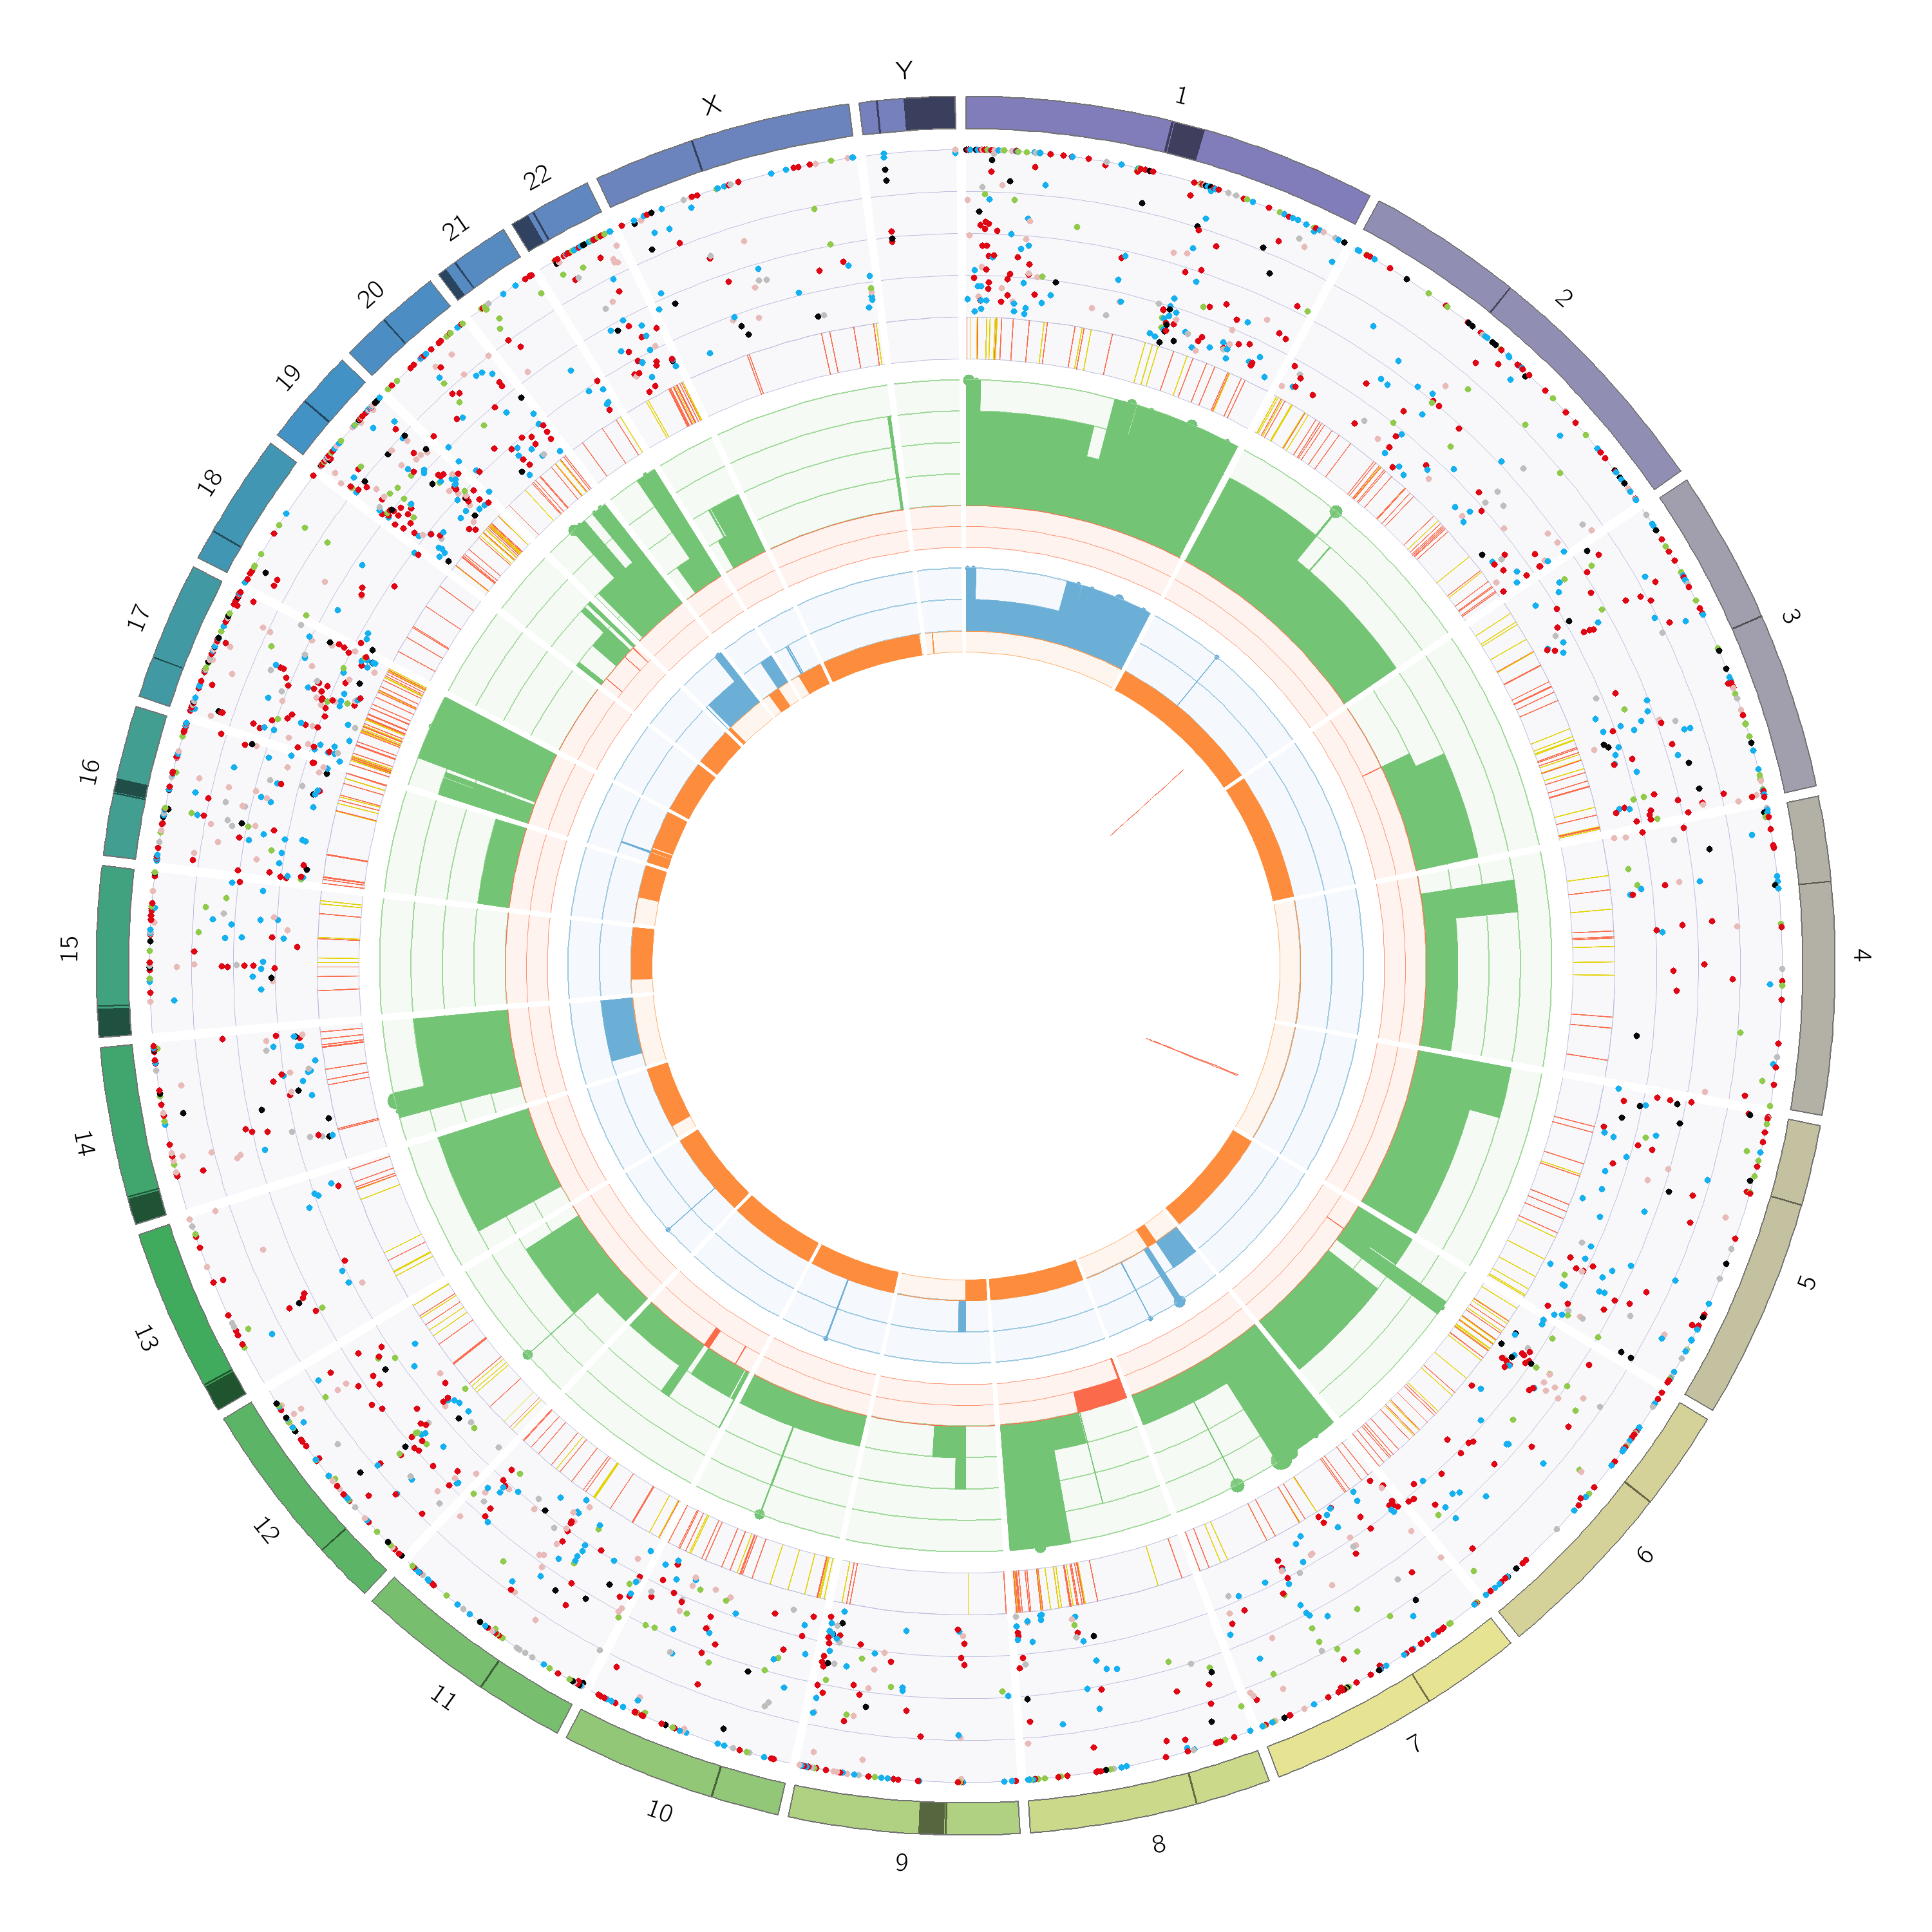
\includegraphics[width=.99\linewidth]{Figures/CASCADE/CA86/CA86-17B037524-1-S.circos.png}
\caption[Circos plot of patient CA-L sample P.1]{Circos plot of patient CA-L sample P.1: outer first ring shows the canonical chromosomes with gaps (centromere, heterochromatin,...) highlighted as darker areas; second ring visualises all somatic SNVs corrected for tumour purity and scaled from 0 to 1, the colour representing the base change of SNV like in \protect\textcite{Alexandrov2013}; vertical lines directly under the SNVs symbolise InDels, with yellow for insertions and red for deletions; the third ring shows the total copy number alterations, with green showing a copy number gain and red a loss, dots at the outer border show a copy number greater than four; the last ring shows the minor copy number, with blue depicting a gain and orange a loss, this ring allows the detection of copy number neutral changes, like loss of heterozygosity; the center shows all structural variants: translocations in blue, deletions in red, insertions in yellow, tandem duplications in green and inversions in black.} \label{fig:ca86.p1circos}
\end{figure}


\begin{figure}[htp]
\centering
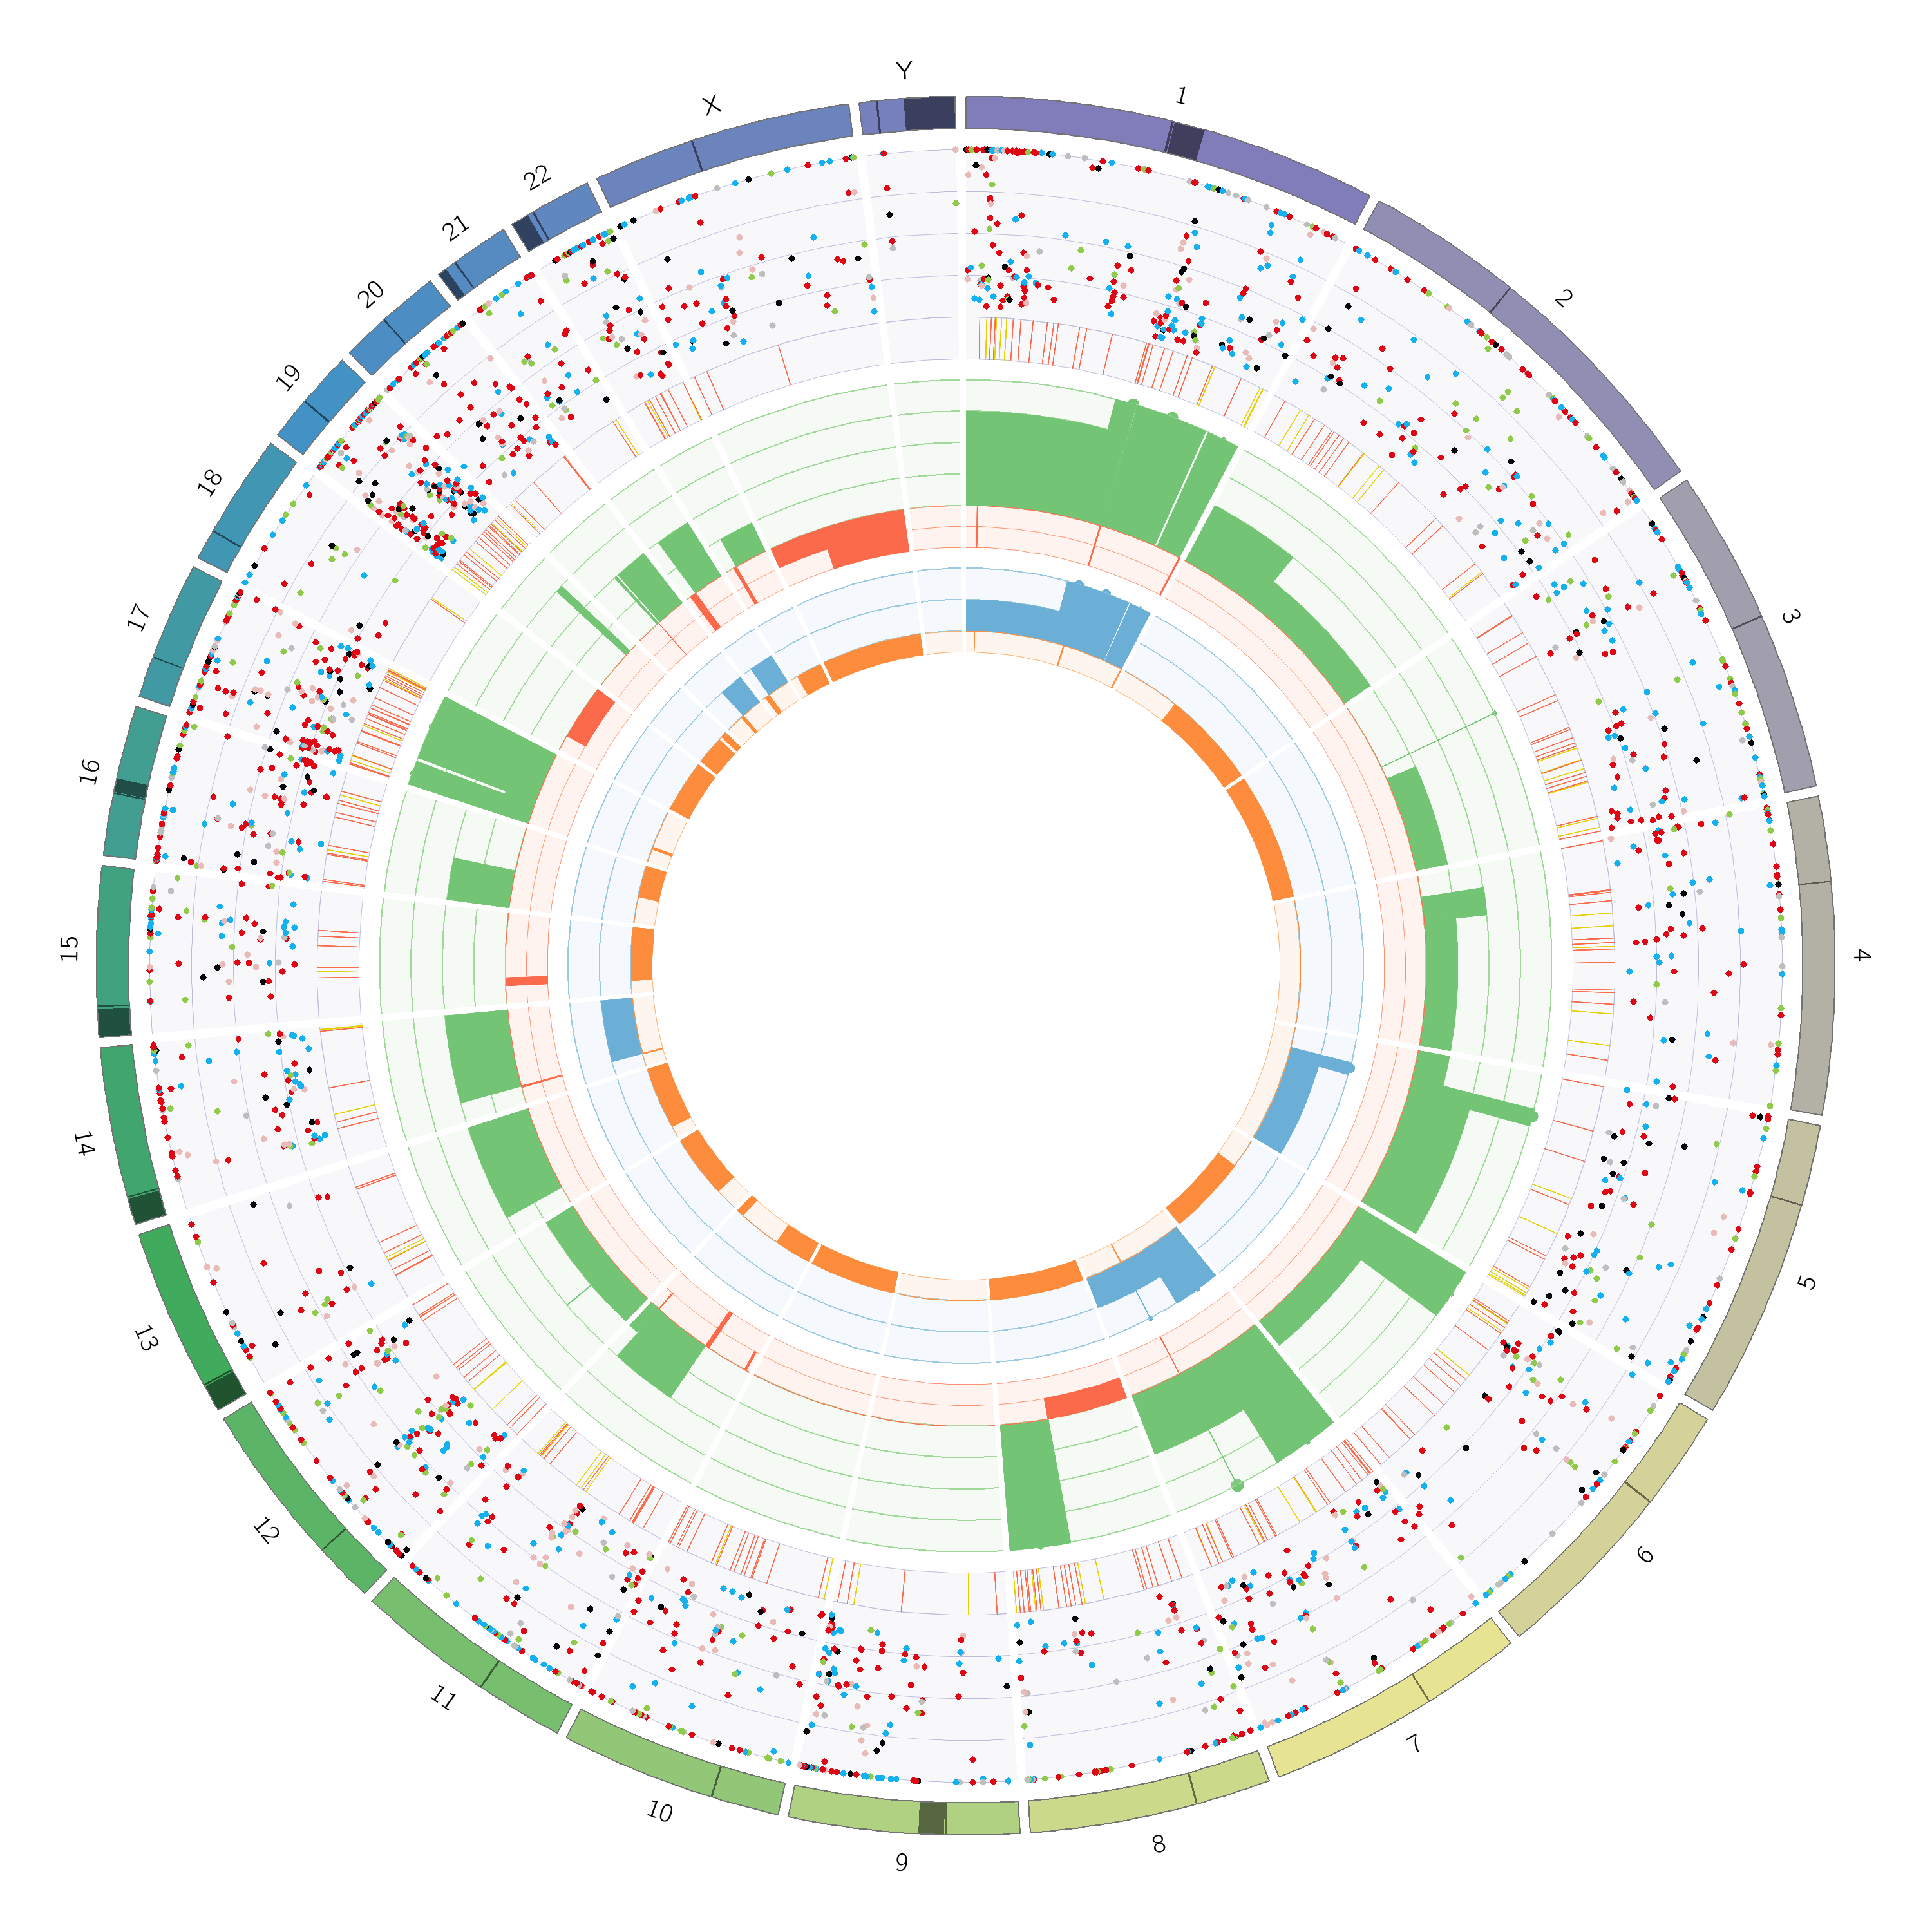
\includegraphics[width=.99\linewidth]{Figures/CASCADE/CA86/CA86-17B037524-1-A.circos.png}
\caption[Circos plot of patient CA-L sample P.2]{Circos plot of patient CA-L sample P.2: outer first ring shows the canonical chromosomes with gaps (centromere, heterochromatin,...) highlighted as darker areas; second ring visualises all somatic SNVs corrected for tumour purity and scaled from 0 to 1, the colour representing the base change of SNV like in \protect\textcite{Alexandrov2013}; vertical lines directly under the SNVs symbolise InDels, with yellow for insertions and red for deletions; the third ring shows the total copy number alterations, with green showing a copy number gain and red a loss, dots at the outer border show a copy number greater than four; the last ring shows the minor copy number, with blue depicting a gain and orange a loss, this ring allows the detection of copy number neutral changes, like loss of heterozygosity; the center shows all structural variants: translocations in blue, deletions in red, insertions in yellow, tandem duplications in green and inversions in black.} \label{fig:ca86.p2circos}
\end{figure}

\begin{table}[ht]
\caption[Copy number analysis results for patient CA-L]{Copy number analysis results for patient CA-L: results are taken from the best fit result of sequenza}\label{tab:ca86cnv}
\centering
\rowcolors{2}{gray!15}{white}
\begin{tabular}{|c|c|c|c|}
\toprule
\hline
 \rowcolor{gray!50}
\textbf{Sample number} & \textbf{purity} & \textbf{ploidy} & \textbf{WG duplication}\\
\hline
 P.1 & \num{0.86} &	 \num{3.3}  & True	\\
 P.2 & \num{0.27} & \num{2.1}  & False \\
 8 & \num{0.96} & \num{3.1}  & True \\
 17A & \num{0.18} & \num{4.2}  & True \\
 26 & \num{0.28} & \num{3.7} & True \\
 \hline
\bottomrule
\end{tabular}
\end{table} 


\begin{figure}[ht]
\centering
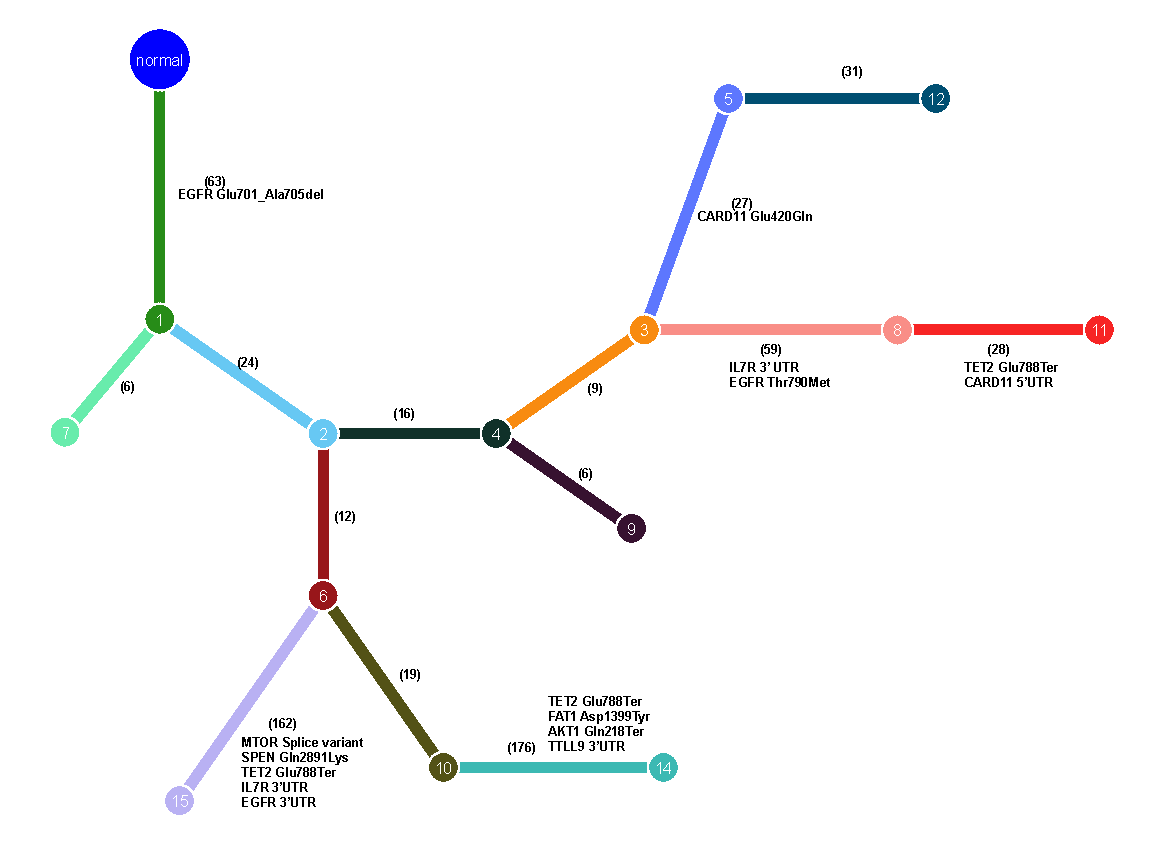
\includegraphics[width=.99\linewidth]{Figures/CASCADE/CA86/CA86.clonaltree.pdf}
\caption[Clonal evolutionary tree CA-L]{Clonal evolutionary tree of patient CA-L; Highest support tree for clustered ccf clones generated with PhylogicNDT; Support for clone is shown in parenthesis; Major driver alterations of cluster were annotated; Clusters with less than 5 supporting variants were discarded.} \label{fig:ca86.clonalTree}
\end{figure}

\begin{figure}[ht]
\centering
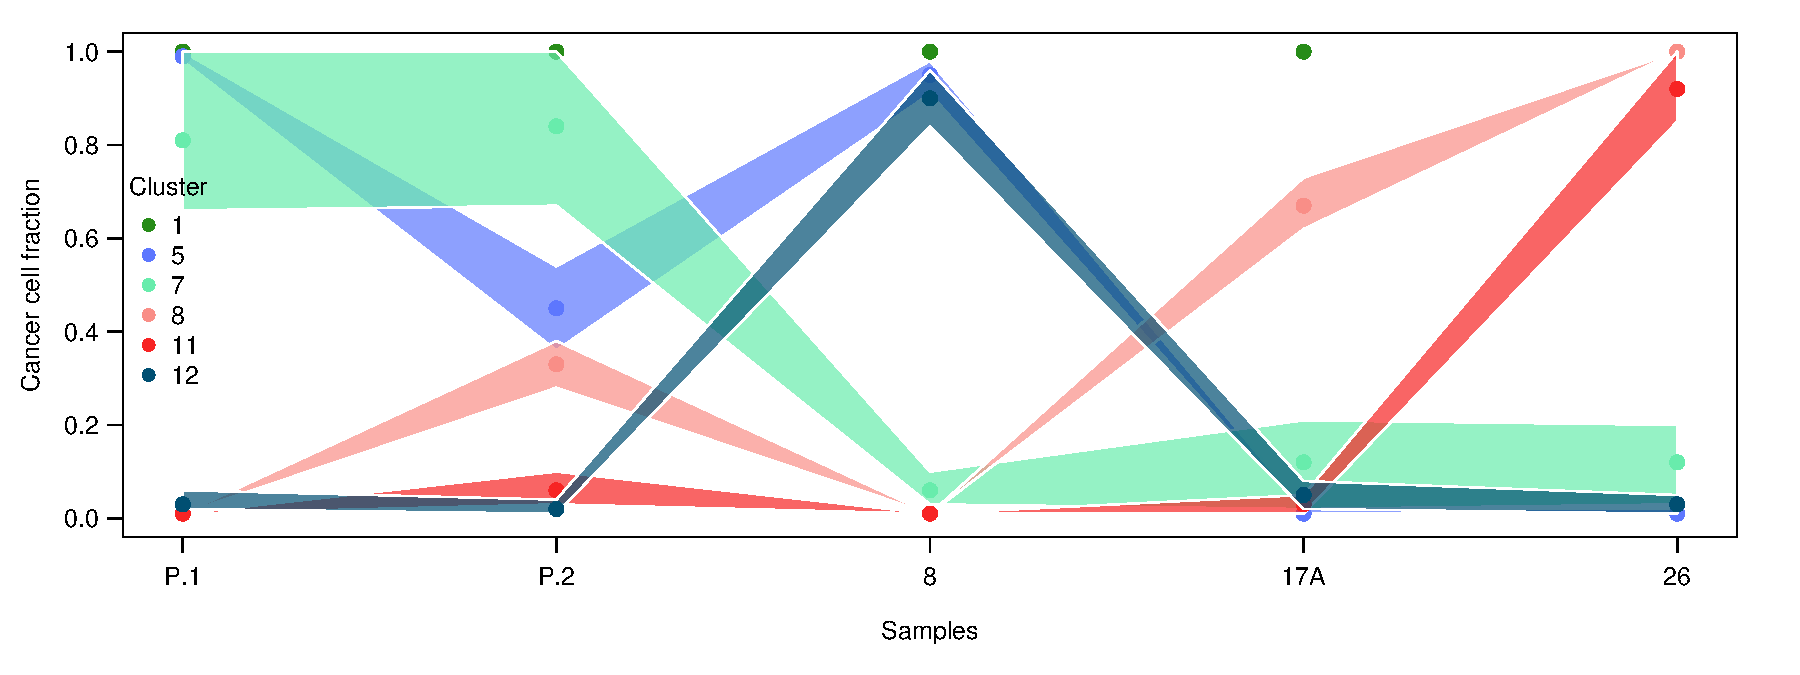
\includegraphics[width=.99\linewidth]{Figures/CASCADE/CA86/CA86.ccf_cluster.pdf}
\caption[Cancer cell fraction of mutation clusters of clonal tree for patient CA-L]{Cancer cell fraction of mutation clusters of clonal tree for patient CA-L; transparent polygons show the 95\% confidence intervals. Clusters and cluster colours are taken from \protect\autoref{fig:ca86.clonalTree}} \label{fig:ca86.ccfCluster}
\end{figure}



Clonal deconvolution with PhylogicNDT showed a split into clusters 6 and 2 from the initial clone with both the initiating \textit{EGFR} deletion and the \textit{TP53} ``stop gained`` mutation. While cluster 6 is present in all samples, the small cell transformed samples P.1 and 8 show a much lower cancer cell fraction, suggesting a correlation. Cluster 2 was then split again in to cluster 4 and a successive evolution of cluster 7 to cluster 30. While cluster 4 shows a similar pattern to cluster 6, the high variability of confidence intervals made assessment challenging. Cluster 4 and 6 could possibly be resolved into the same clone with deeper sequencing. Finally cluster 5 and 13, the progeny of cluster 30 allowed the perfect split of samples into small cell transformed and adenocarcinoma samples. Samples P.2, 17A, and 26, where the presence of cluster 13 could be observed were adenocarcinoma. However, the presence of cluster 5, which was only present in the small cell samples at autopsy suggested an incomplete micro-dissection of the progression sample (\Autoref{fig:ca86.clonalTree,fig:ca86.ccfCluster}). Surprisingly, there was no known genetic determinant found, which explained the split into EGFR~T790M positive and small cell transformed lung cancer. In contrast, it is likely that the priming for for transformation or remaining adenocarcinoma was epigenetic~\cite{Fennell2021,Suva2013}.



%we clear all floats before we go to the next section
\cleardoublepage